\documentclass[a4paper,oneside,14pt]{scrbook}

\usepackage[utf8]{inputenc}
\usepackage[russian]{babel}
\usepackage{indentfirst}
\usepackage[colorlinks=true]{hyperref}
\usepackage{graphicx}
\usepackage{amsmath}
\usepackage{guitar}
\usepackage{musixtex}

\usepackage{etex} %эта магическая херь избавляет от переполнения регистров TeX'а

%вставка изображений из metapost (post script)
\DeclareGraphicsRule{*}{mps}{*}{}

%пометка черновика (закомментировать три строки ниже для релиза)
\usepackage{draftwatermark}
\SetWatermarkScale{1.5}
\SetWatermarkText{$\beta$-версия от \today}

\title{О музыке и шестиструнной гитаре для аналитического ума}
\author{М.~М.~Шихов}
\date{\today}

\newtheorem{Example}{Пример}[chapter]
\newtheorem{Rule}{Правило}[chapter]
\newtheorem{Definition}{Определение}[chapter]
\newtheorem{Note}{Заметка}[chapter]

%определённые мной команды логической разметки
\newcommand{\myNemph}[1]{{\small{\emph{#1}}}}


\begin{document}
    \maketitle
    \tableofcontents

    \chapter*{Введение}
\addcontentsline{toc}{chapter}{Введение}

Иногда человек, сталкивавшийся с музыкой только как слушатель, вдруг приходит к мысли: <<А почему бы мне не попробовать научиться \emph{играть} на инструменте X?>>. И тут он открывает для себя параллельную вселенную.

Через некоторое время, если этот человек не прибегает к помощи знающих людей, и ему не везет с учебниками (самоучителями, обучающими видео в Интернет и т.д.), он понимает, что в этой вселенной ему нет места.

Особенно остро это понимают люди с инженерным (математическим, техническим и т.д.) образованием. Им хочется найти в музыке целостную систему, знания, обобщения, красивые законы, а не обилие разрозненных фактов.

Погружаясь в музыкальню тему, человек с аналитическим мышлением быстро офигевает от необходимости зубрить и принимать на веру практически всё. Не находя в учебниках ответа на фундаментальные вопросы <<зачем и почему?>>, он закономерно посылает музыку подальше.

Прекрасные музыканты, которые в свое время прошли пытку музыкальной школой (может быть училищем или даже консерваторией), имели достаточно времени, чтобы подсознательно объяснить себе некоторые вещи и смириться с ними. Не каждый человек задумывается над тем, с чем просто сжился. Привычные вещи люди чаще перестают замечать, а не стараются в них разобраться.

И если новичку с аналитическим типом мышления вдруг не везет с учителем, который в силу изложенных выше причин гораздо больше \emph{чует}, чем \emph{знает}, то новичок очень быстро убеждается в инопланетности, а то и вовсе в избранности музыкантов.

Нет никакой избранности, большинство музыкантов --- Земляне, а в музыкальной вселенной можно не только выжить, но и жить счастливо, ибо там есть законы и гармония! 

В чем и попробуем убедиться:

\begin{music}
    \startextract
    \notes\qu{cdefghi}\enotes
    \endextract
\end{music}
    %что-зачем
    \chapter{Музыка? Нет, не слышали\ldots}
\label{ch:music}

Когда автор учился в ВУЗе, преподаватель интеллектуальной собственности\footnote{Это о всяких там авторских правах и изобретениях} дал студентам красивый критерий, чтобы отличать произведение искусства от произведения техники: <<ребята, произведение искусства со временем становится только дороже, а техническое решение --- дешевле>>. Ну, то есть картины Леонардо Да-Винчи будут уходить с аукционов за космические деньги, а вот модель вашего крутого компа (телефона, и даже версия программы, которую вы напишете, и т.д.) со временем даром никому не будет нужна. 

К чему это я? Существует огромное количество сомнительных критериев отделить почётное \emph{искусство} от стрёмной науки. Выше был экономический критерий, мол искусство дорожает. 

А вот, например, критерий неврологический. В вашей черепушке сидит мозг с двумя полушариями: левым --- аналитическим, сравнивающим, разделяющим и рассуждающим, и правым --- синтезирующим, творческим, эмоциональном и витающем в облаках. И вот в какую сторону ваша черепушка перевесит, тем вы и будете: клонит влево --- физик, а вправо --- лирик. Физик разумный, а лирик эмоциональный. Физик в науке, лирик в искусстве. И дойдем в своих рассуждениях до абсурда: в искусстве уму не место, а наука лишена эмоций!

И вот у многих уже есть повод сказать: не лезьте в музыку с математикой, не путайте искусство с наукой! 

Ой, да ладно! Друзья, музыка волнует наши чувства только потому, что математика внутри вас\footnote{Да и наукой (настоящей) люди занимаются чисто по эмоциональным причинам: им любопытно!}. Эмоции и разум растут от одного корня.

\begin{Definition}[Музыка]
    Музыка начинается тогда, когда звуки \emph{правильной} высоты\footnote{\emph{Нота} обозначает звук нужной высоты} с \emph{правильной} громкостью\footnote{В музыке это называется \emph{акцентом}} звучат в \emph{правильное} время\footnote{В музыке есть определенный \emph{ритм}}.
\end{Definition}

Итак, разберемся с \emph{правилами} для высоты, громкости и времени звучания звуков.


\section{Немного <<правильной>> физики}

Если задеть гитарную струну, вы услышите звук. Струна начнет колебаться и создавать вокруг себя периодические сжатия и разряжения воздуха, которые затем будут распространяться во все стороны от струны. Этот эффект называется звуковой \emph{волной}\footnote{В отличие от волн на поверхности воды, которые распространяются <<кругами>> от упавшего в воду предмета, звуковые волны имеют эффект 3D и распространяются <<шарами>> --- во все стороны от источника звука.}. Волна распространяется от источника звука со скоростью примерно 340 метров в секунду.

Количество периодических сжатий (или разряжений) в секунду физики называют частотой, а лирики --- высотой звука. То есть чем чаще колеблется струна, тем \emph{выше} звук, который она издаёт. Ну и наоборот: чем реже колеблется струна, тем \emph{ниже} звук\footnote{И если частоту можно измерить точно, то оценки выше-ниже --- относительны и субъективны. Басом (низким голосом) разговаривает огромный спокойный мужик, а истеричка визжит на высоких тонах}.

Если вы дернете струну сильнее, она зазвучит громче. Струна от этого не станет колебаться быстрее, нет, она издаст звук той же высоты, что и обычно. Она будет совершать колебания с большим размахом --- физики скажут: <<с большей амплитудой>>. Из-за этого сжатия и разряжения воздуха усилятся. И, когда звук дойдет до уха слушателя, эти сжатия и разряжения начнут сильнее шатать барабанную перепонку в ухе и\ldots И физика кончится, а начнутся биология и информатика.

Человеческое ухо может различать такие характеристики звуковой волны, как её частота и амплитуда. Незатухающие колебания одной неизменной частоты, человек услышит как тон\footnote{Например, заходящий на посадку на ваше ухо комар, машет крыльями примерно 659.26 раз в секунду и вы слышите незабываемое Ми второй октавы!}. А амплитуду волны (размах колебаний) --- как громкость. Человеческий слуховой аппарат воспринимает ограниченный диапазон частот (примерно от 16 до 20000 Гц), а восприятие громкости звука, если честно, зависит не только от амплитуды звуковых колебаний, но и от частоты.


\section{Как звучит струна? Или правильная высота}

TODO: Равномерно-темперированный строй.

TODO:
% Частота от звука к звуку повышается в \emph{геометрической} прогрессии. То есть частота каждого следующего музыкального звука в \[\sqrt[12]{2}\approx 1,059463\] больше частоты звука предыдущего.
% 
% Так, следующий за ЛЯ первой октавы, звук ЛЯ-диез, имеет частоту $440\cdot\sqrt[12]{2}\approx 466,16$ герц. Звук СИ имеет частоту $440\cdot(\sqrt[12]{2})^2\approx 493,88$. И так далее, например, ЛЯ второй октавы имеет, как и положено, в два раза большую частоту, чем ЛЯ первой октавы: $440\cdot(\sqrt[12]{2})^{12}=440\cdot 2=880$ Гц.
% 
% Задав эталонную частоту любого музыкального звука, частоты для всех остальных звуков можно \emph{вычислить}.


Слияние звуков кратной частоты.

Октава.

\section{Маршируем? Вальсируем? Правильная громкость}
\label{sec:music:sounds}


\section{Еще и глушить надо? Правильное время}



    %что есть музыка
    \chapter{Элементы нотной грамоты}
\label{ch:note}

Нотную запись нельзя назвать эталоном простоты. Она, несомненно, сложнее, чем могла бы быть. Так уж сложилось, и, уважая гениальность предков, мы изучим её такой, какая она есть.


\section{Немного теории}

\emph{Нота} --- это \emph{обозначение} (способ записи, если хотите) колебаний воздуха с некоторой постоянной частотой. Такие колебания некоторое время производит гитарная струна после щипка --- особого удара пальцем по ней. Нота звучит \emph{выше}, если частота колебаний струны \emph{больше}. Ну а низкая нота --- это колебания с малой частотой. Например, в соответствии с международным стандартом, струна, звучащая на ноте Ля первой октавы (о октавах позже) колеблется с частотой 440 герц, то есть совершает 440 полных колебаний в секунду\footnote{Допускается вольность принять за Ля первой октавы любую частоту из интервала от 430 до 450 герц. Многие фанатики утверждают, что Ля в 432 Гц от Бога (и оздоравливающе действует на организм), а стандартизованная 440 Гц --- от Сатаны, соответственно (и разрушает психику).}.

Человеческое ухо способно различать такие характеристики звуковой волны, как её частота и амплитуда. Незатухающие колебания одной неизменной частоты, человек услышит как тон\footnote{Например, заходящий на посадку на ваше ухо комар, машет крыльями примерно 659.26 раз в секунду и вы слышите незабываемое Ми второй октавы!}. А амплитуду волны (размах колебаний) --- как громкость. Человеческий слуховой аппарат воспринимает ограниченный диапазон частот (примерно от 16 до 20000 Гц), а восприятие громкости звука, если честно, зависит не только от амплитуды звуковых колебаний, но и от частоты.

В Русской традиции принято использовать \emph{семь} обозначений для кодирования нот (которые приведены ниже в порядке возрастания частоты колебаний (высоты звука)): 
\begin{center}
    До, Ре, Ми, Фа, Соль, Ля, Си. 
\end{center}

Так что получается, мы имеем дело всего с семью звуками? Конечно нет!

Пусть мы дошли до последней ноты Си и... И текущая \emph{октава} кончилась. Но началась следующая! В следующей октаве все повторится: До, Ре, Ми, Фа, Соль, Ля, Си. Только вот частота звука для соотвествующей ноты будет в \emph{два} раза больше! То есть, например, ноте Ля второй октавы соответствует вдвое большая частота (880 Гц), чем ноте Ля первой октавы (стандартные 440 Гц).

Октавы, использующиеся в музыке, имеют следующие названия.
\begin{center}
    \begin{tabular}{ll}
        \hline\hline
        Название октавы         & Частота ноты Ля, Гц \\
        \hline\hline
        
        Субконтроктава          & 27.5 \\
        Контроктава             & 55   \\
        \emph{Большая октава}   & 110  \\
        \emph{Малая октава}     & 220  \\
        \emph{Первая октава}    & \fbox{440}  \\
        \emph{Вторая октава}    & 880  \\
        Третья октава           & 1760 \\
        Четвертая октава        & 3520 \\
        Пятая октава            & 7040 \\
        \hline
    \end{tabular}
\end{center}

В таблице \emph{выделены} те октавы, которые входят в диапазон шестиструнной гитары. Справедливости ради следует сказать, диапазон звучания шестиструнной гитары полностью включает лишь малую и первую октавы.

А вот теперь пришло время для секретов: традиционно в октаве принято выделять \emph{двенадцать} нот! 

Погодите, погодите, скажете вы: <<До, Ре, Ми, Фа, Соль, Ля, Си>> --- семь нот! И октава названа, вероятно, не просто так: <<octo>> --- это восемь, восьмая нота! Все логично!

Так все шоке, но молчат! <<До, Ре, Ми,\ldots>> --- это \emph{названия} лишь семи нот из 12. А вот (12-7)=5 нот не удостоились отдельных имен. Итак, оставшиеся 5 нот находятся между упорядоченными по частоте нотами:
\begin{enumerate}
    \item До и Ре (эта нота может быть названа либо До-диез, либо Ре-бемоль)
    \item Ре и Ми (Ре-диез или Ми-бемоль)
    \item Фа и Соль (Фа-диез или Соль-бемоль)
    \item Соль и Ля (Соль-диез или Ля-бемоль)
    \item Ля и Си (Ля-диез или Си-бемоль)
\end{enumerate}    

Как видно, эти <<промежуточные>> ноты могут называться двояко. Какое из имен выбрать? Постараюсь ответить кратко: если вы читаете этот текст и узнаёте для себя что-то новое, то вам позволительно использовать любое\footnote{Это как грамотность в Русском языке: надеть или одеть? Одеть Надежду, надеть одежду! Чужак не осилит. Так что называйте как хотите, знающие друзья поправят, если что. Только помалкивайте на какой-нибудь музыкальной конференции в кругу маститых классических исполнителей.}! Все 12 нот октавы в порядке увеличения высоты:
\begin{center}
    До, \emph{До-диез}, Ре, \emph{Ре-диез}, Ми, Фа, \emph{Фа-диез}, Соль, \emph{Соль-диез}, Ля, \emph{Ля-диез}, Си
\end{center}

Частота от ноты к ноте повышается в \emph{геометрической} прогрессии. То есть частота звука каждой следующей ноты в \[\sqrt[12]{2}\approx 1,059463\] больше частоты звука предыдущей. 

Так, следующая за нотой Ля первой октавы, нота Ля-диез, имеет частоту $440\cdot\sqrt[12]{2}\approx 466,16$ герц. Нота Си имеет частоту $440\cdot(\sqrt[12]{2})^2\approx 493,88$. И так далее, например, Ля второй октавы имеет, как и положено, в два раза большую частоту, чем Ля первой октавы: $440\cdot(\sqrt[12]{2})^{12}=440\cdot 2=880$ Гц.

Задав эталонную частоту любой ноты, частоты для всех остальных нот можно вычислить.

В учебниках говорится, что добавление суффикса <<диез>> означает повышение частоты исходной ноты на <<полутон>>, что математически соответствует увеличению частоты в $\sqrt[12]{2}$ раз. И это в целом правильно, только обычно ученики начинают думать, что между соседними нотами из списка До, Ре, Ми, Фа, Соль, Ля, Си --- расстояние в два <<полутона>> (то есть в <<тон>>)! Не забыайте, что между нотами Ми и Фа, а также между Си и До <<промежуточных>> нот нет и расстояние между ними --- один <<полутон>>. 

Как видно из реальной последовательности, следуя такой логике, например, Ми-диез --- это Фа, или Си-диез --- это До следующей октавы. Обычно ноту Фа, конечно никто не называет Ми-диез --- это оскорбительно, но никто и не запрещает так делать. 

То же самое можно сказать и о суффиксе <<бемоль>>, он понижает ноту на полутон. И, например, До-диез, это та же нота, что и Ре-бемоль. А если вы хотите оскорбить ноту Ми, то назовите её Фа-бемоль. Если вы хотите прочитать все 12 нот в обратном порядке, то грамотно будет использовать суффикс <<бемоль>>, а не <<диез>>:

\begin{center}
Си, Си-бемоль, Ля, Ля-бемоль, Соль, Соль-бемоль, Фа, Ми, Ми-бемоль, Ре, Ре-бемоль, До.
\end{center}


\section{Устройство гитары}

Мы разобрались с теорией нот в предыдушем разделе, теперь коснемся особенностей устройства гитары, которые позволяют извлекать ноты именно такими, какими они и должны быть. 

Для начала стоит взглянуть на рисунок \ref{fig:guitarConstruction} и запомнить, что значат незнакомые вам обозначения.

\begin{figure}[!ht]
    \centering
    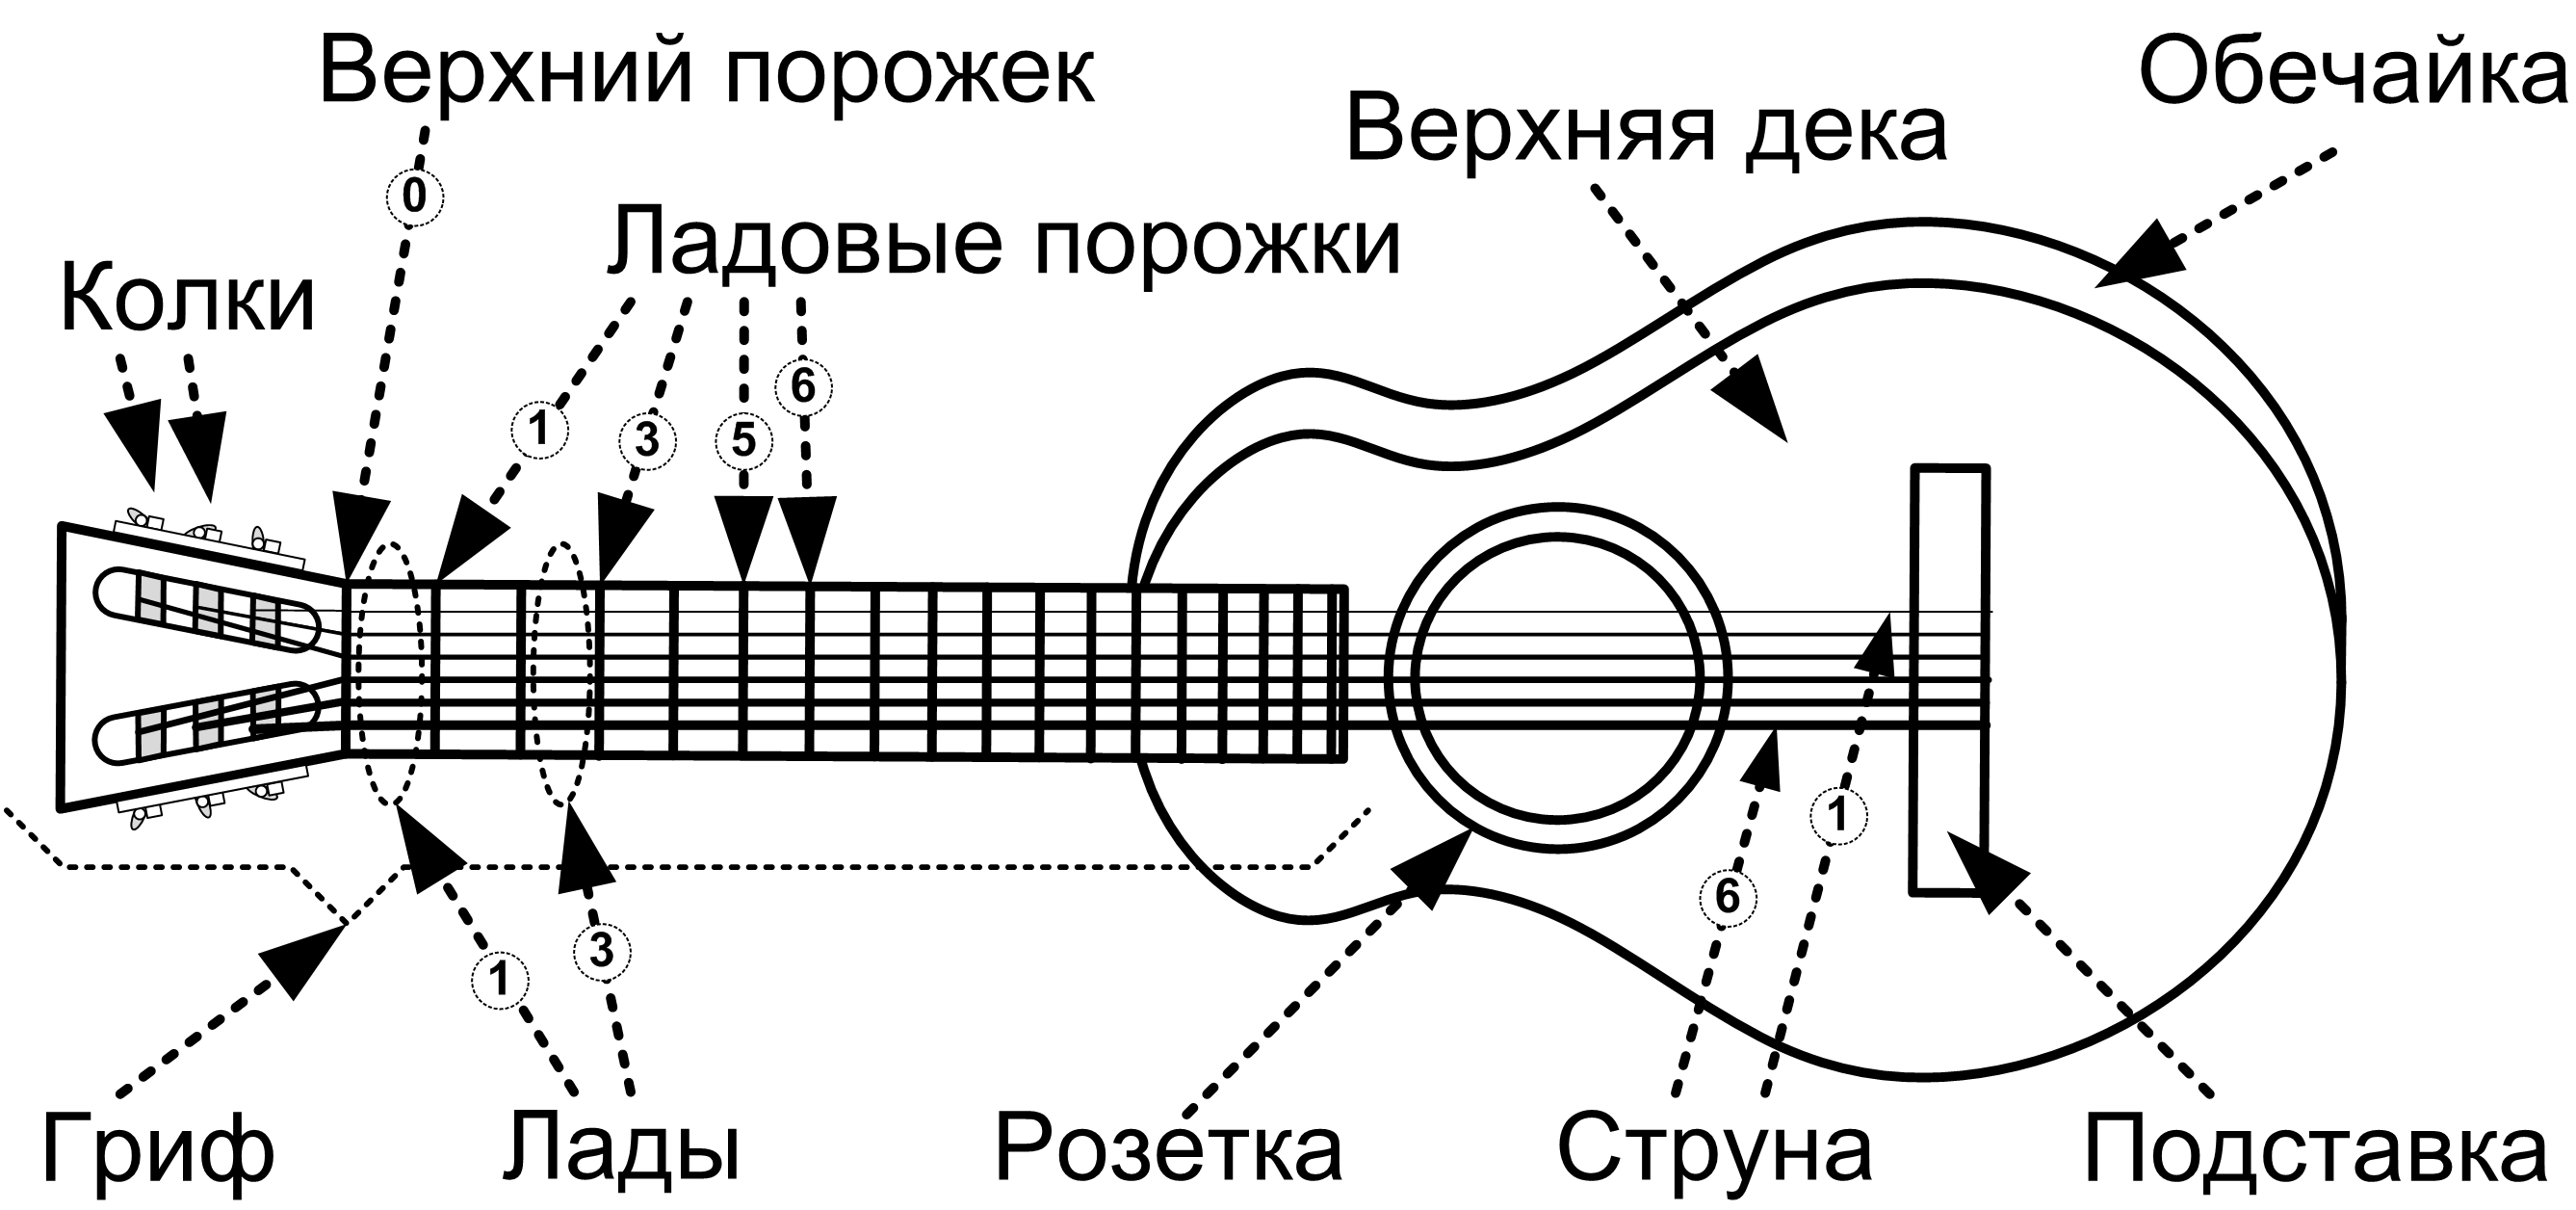
\includegraphics{fig/guitar-construction} 
    \caption{Устройство гитары}\label{fig:guitarConstruction}
\end{figure} 

Любая открытая\footnote{То есть не зажатая ни на каком ладу} струна гитары звучит строго определенной нотой (о настройке гитары поговорим позже). Лады на грифе (промежутки между порожками), равно как и \emph{ладовые порожки} считаются от \emph{верхнего} порожка: 1,2,3,\ldots и т.д. То есть <<зажать струну на первом ладу>> значит, что вы ставите палец на струну, на первый лад, то есть между верхним порожком и первым ладовым\footnote{Чем ближе к первому ладовому, тем лучше. Таким образом и звук будет чище, и рука уставать будет меньше. Ставить палец сверху на порожек не стоит --- звук будет <<глохнуть>>. Правда иногда именно это и требуется. Но в начале обучения стоит ставить палец на ладу ближе к тому порожку, от которого идет <<звучащая>> часть струны. Добивайтесь чистого звука.} и нажимаете до тех пор, пока струна не прижмётся к первому ладовому порожку. Но нам важно сейчас не то, как правильно зажимать струну. 

Важно понять, что каждый следующий лад повышает звук на струне на <<полутон>>. В октаве 12 нот и каждая звучит на струне на своём ладу. На дветадцатом ладу звучит нота открытой струны, только выше на октаву.

Из физики известно, что частота колебаний струны обратно пропорциональна её длине\footnote{Надо честно заметить, что частота колебаний струны зависит также и от силы её натяжения, которая меняется, когда струну <<зажимают>> на ладу. Но это влияние столь незначительно, что им можно пренебречь.}. Стало быть, чтобы частота издаваемого струной звука \emph{увеличилась} вдвое (а языком музыки --- чтобы нота зазвучала октавой выше), надо вдвое \emph{укоротить} струну. 

Зажимая струну на 12 ладу (языком музыки --- повышая ноту открытой струны на октаву), вы укарачиваете звучащую часть струны вдвое. Линейка в помощь, если не верите\footnote{Конечно нужно мерять только звучащую (колеблющуюся часть) струны от опоры на подставке до 12-го ладового порожка.}.

Конечно, частота колебаний струны зависит также и от силы её натяжения. Сила натяжения струны регулируется колками на грифе, когда гитару настраивают. Играя, гитарист только меняет длину звучащего участка струны, зажимая струны на ладах. Редкие психи\footnote{Конечно, имелось в виду: \emph{мастера}! Прим. ред.} крутят колок во время исполнения, добиваясь сомнительных\footnote{Конечно, имелось в виду: \emph{удивительных}! Прим. ред.} эффектов.

Исходя из того, что частота каждой следующей ноты в $\sqrt[12]{2}$ больше предыдущей, запишем формулу длины струны ($L$) от места крепления струны к подставке до $n$-го ладового порожка:

\[L(n)=\frac{L}{(\sqrt[12]{2})^n},\]
где $n$ - номер лада ($0$-й лад соответствует открытой струне), а $L$ --- общая длина струны от подставки до верхнего порожка.


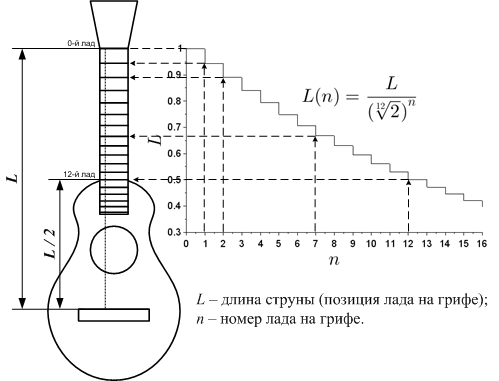
\includegraphics{fig/string-length.png}


Из картинки, надеюсь, ясно, почему ладовые порожки на гитаре расположены не на равном расстоянии друг от друга.

Кстати, некоторые ушастые выпендрёжники говорят, что различают своим сверхмузыкальным слухом больше 12 нот в октаве! И им мало 12 ладов! Есть спрос --- есть предложение: на некоторых гитарах можно заметить дополнительные ладовые порожки между <<каноническими>>, которые позволяют <<всунуть>> дополнительную ноту.


\section{Запись гитарных нот на бумаге}

Чтобы записать ноты, купите нотную тетрадь или на обычном листе начертите нотоносец --- пять параллельных, расположенных друг под другом через равные интервалы (около двух миллиметров) линий:
 

Традиционно ноты для шестиструнной гитаре записываются в скрипичном ключе, который своим хвостиком огибает вторую снизу линию нотоносца, на которой располагется Соль \emph{малой} октавы\footnote{Для других музыкальных инструментов, в первую очередь, для фортепиано, скрипичный ключ показывает положение Соль \emph{первой} октавы, но для гитары, чтобы использовать один нотоносец, ноты пишут на <<фортепианный>> скрипичный нотоносец на октаву выше.}.


\section{Поиск нот на грифе}

\begin{figure}[!ht]
    \centering
    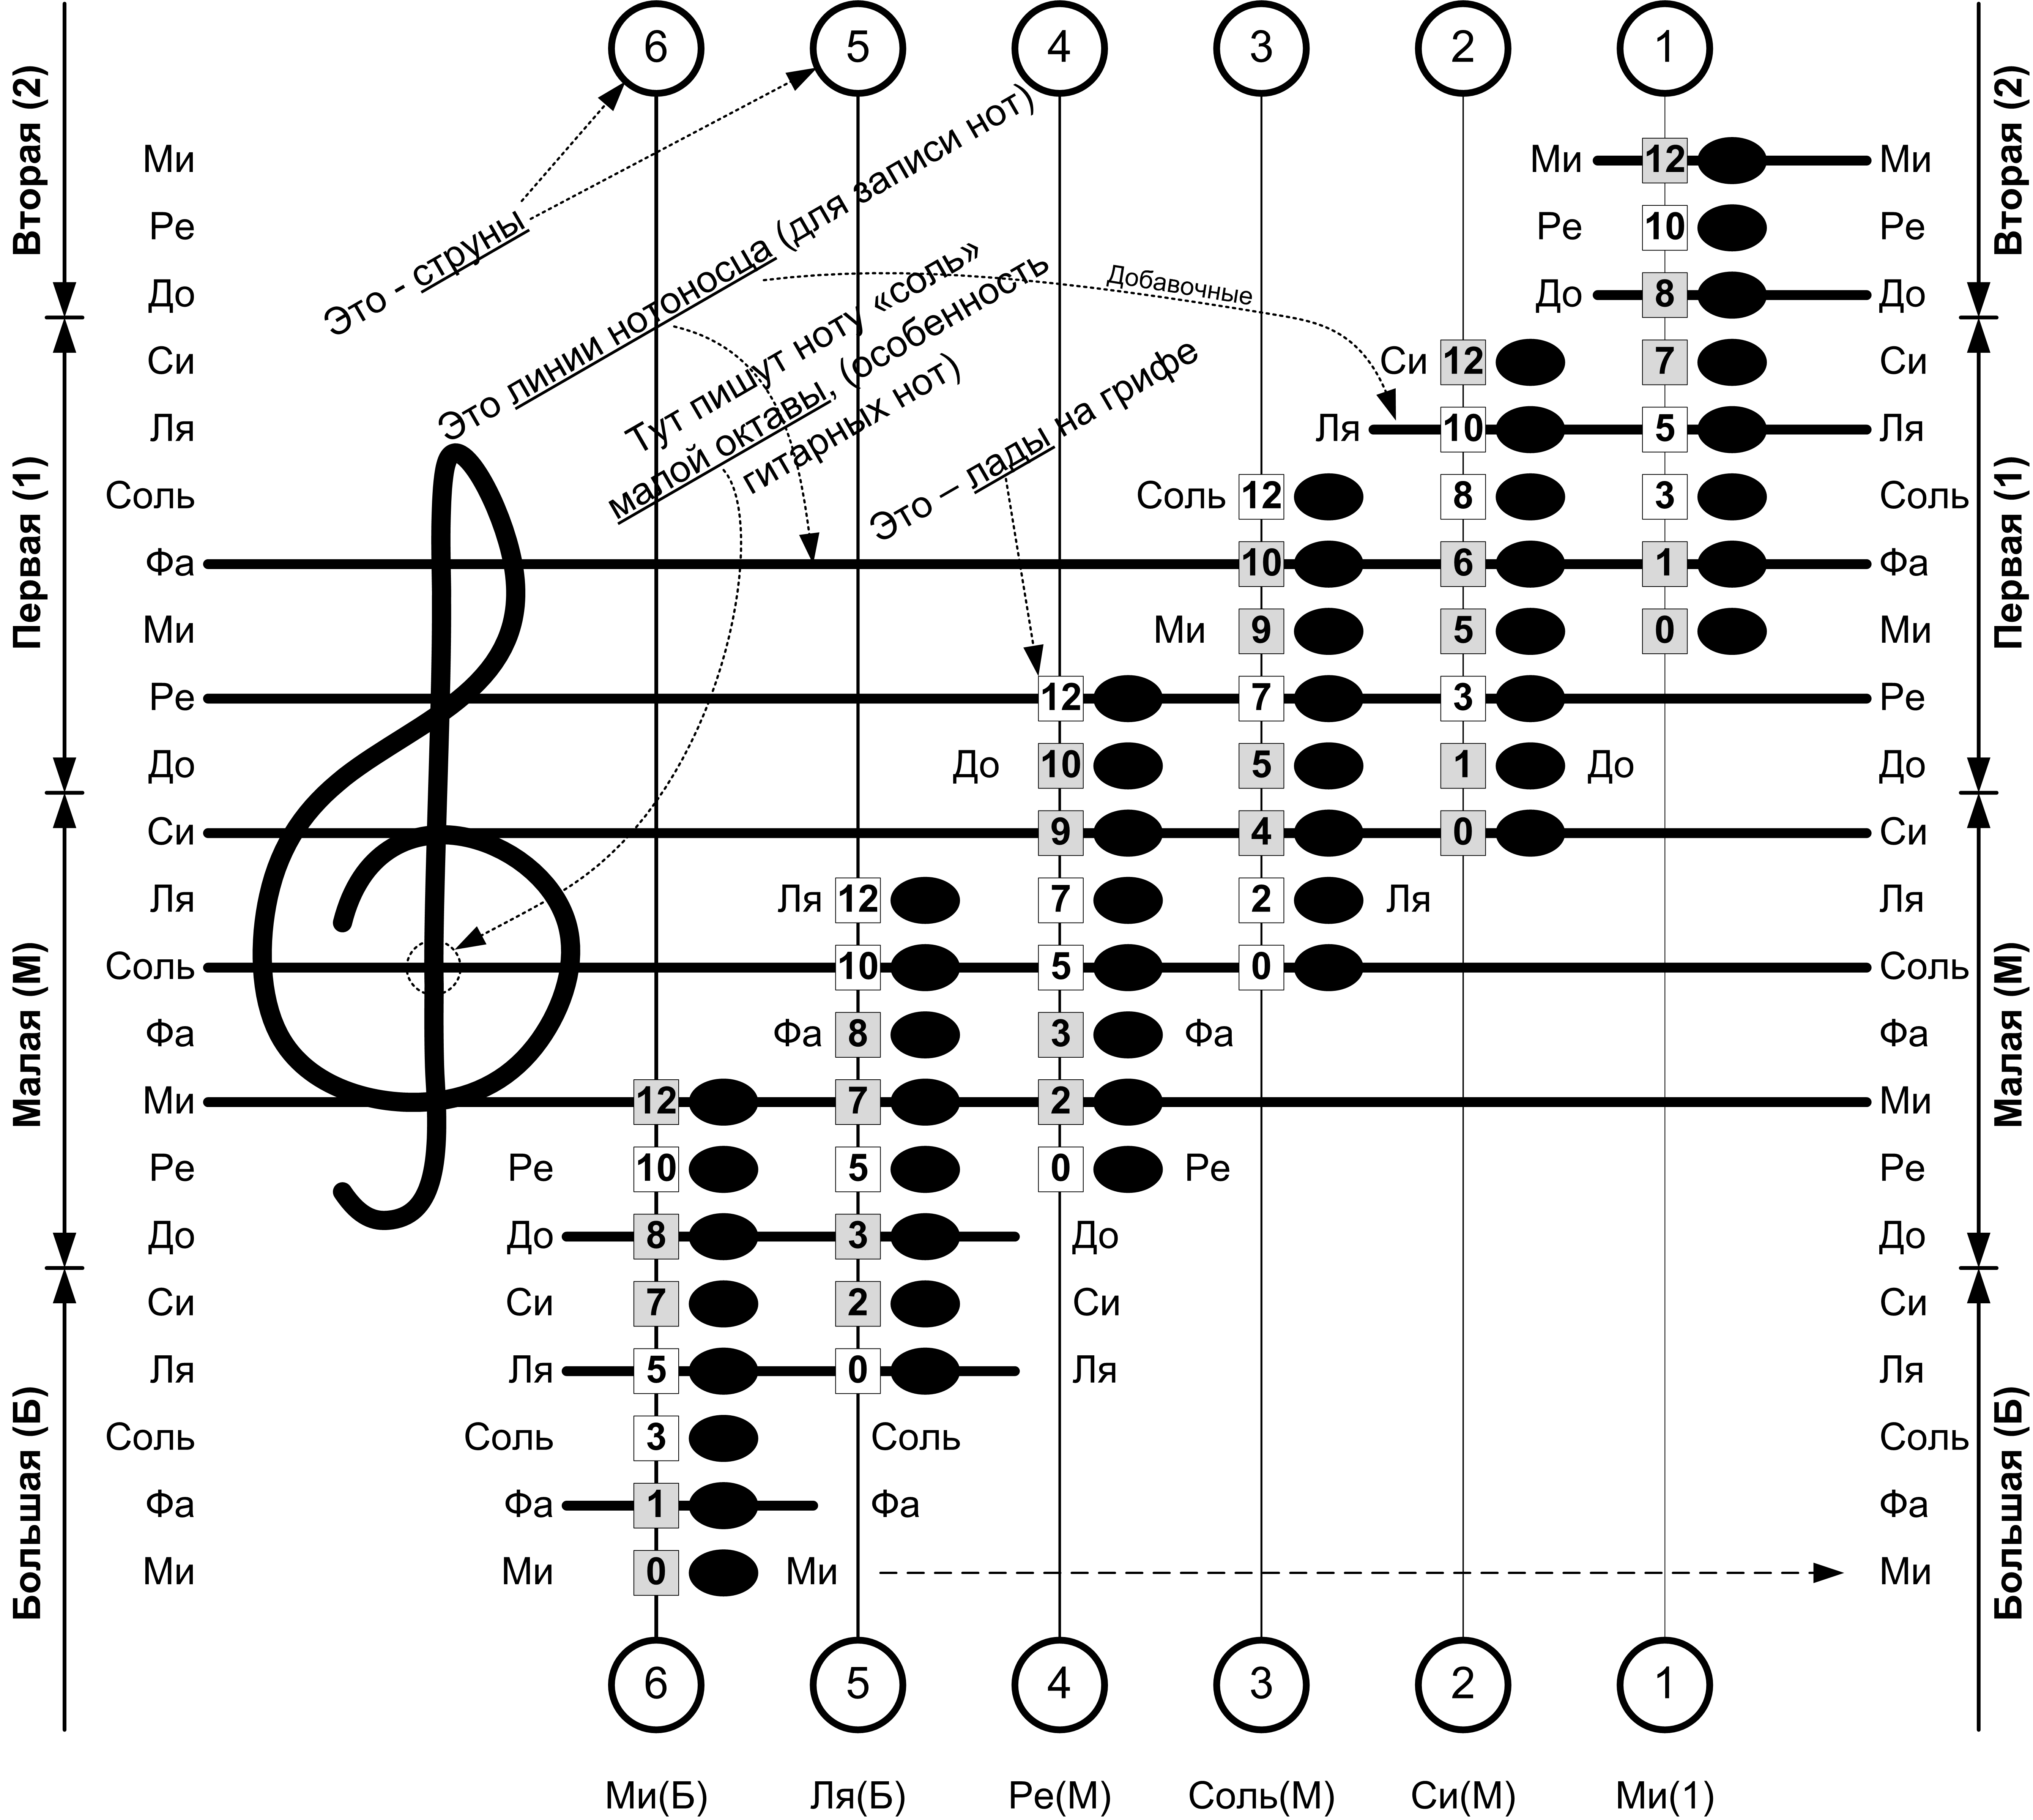
\includegraphics[width=\textwidth]{fig/lad-by-notes} 
    \caption{Ноты на грифе (гриф поперек нотоносца)}\label{fig:ladByNotes}
\end{figure} 

\begin{figure}[!ht]
    \centering
    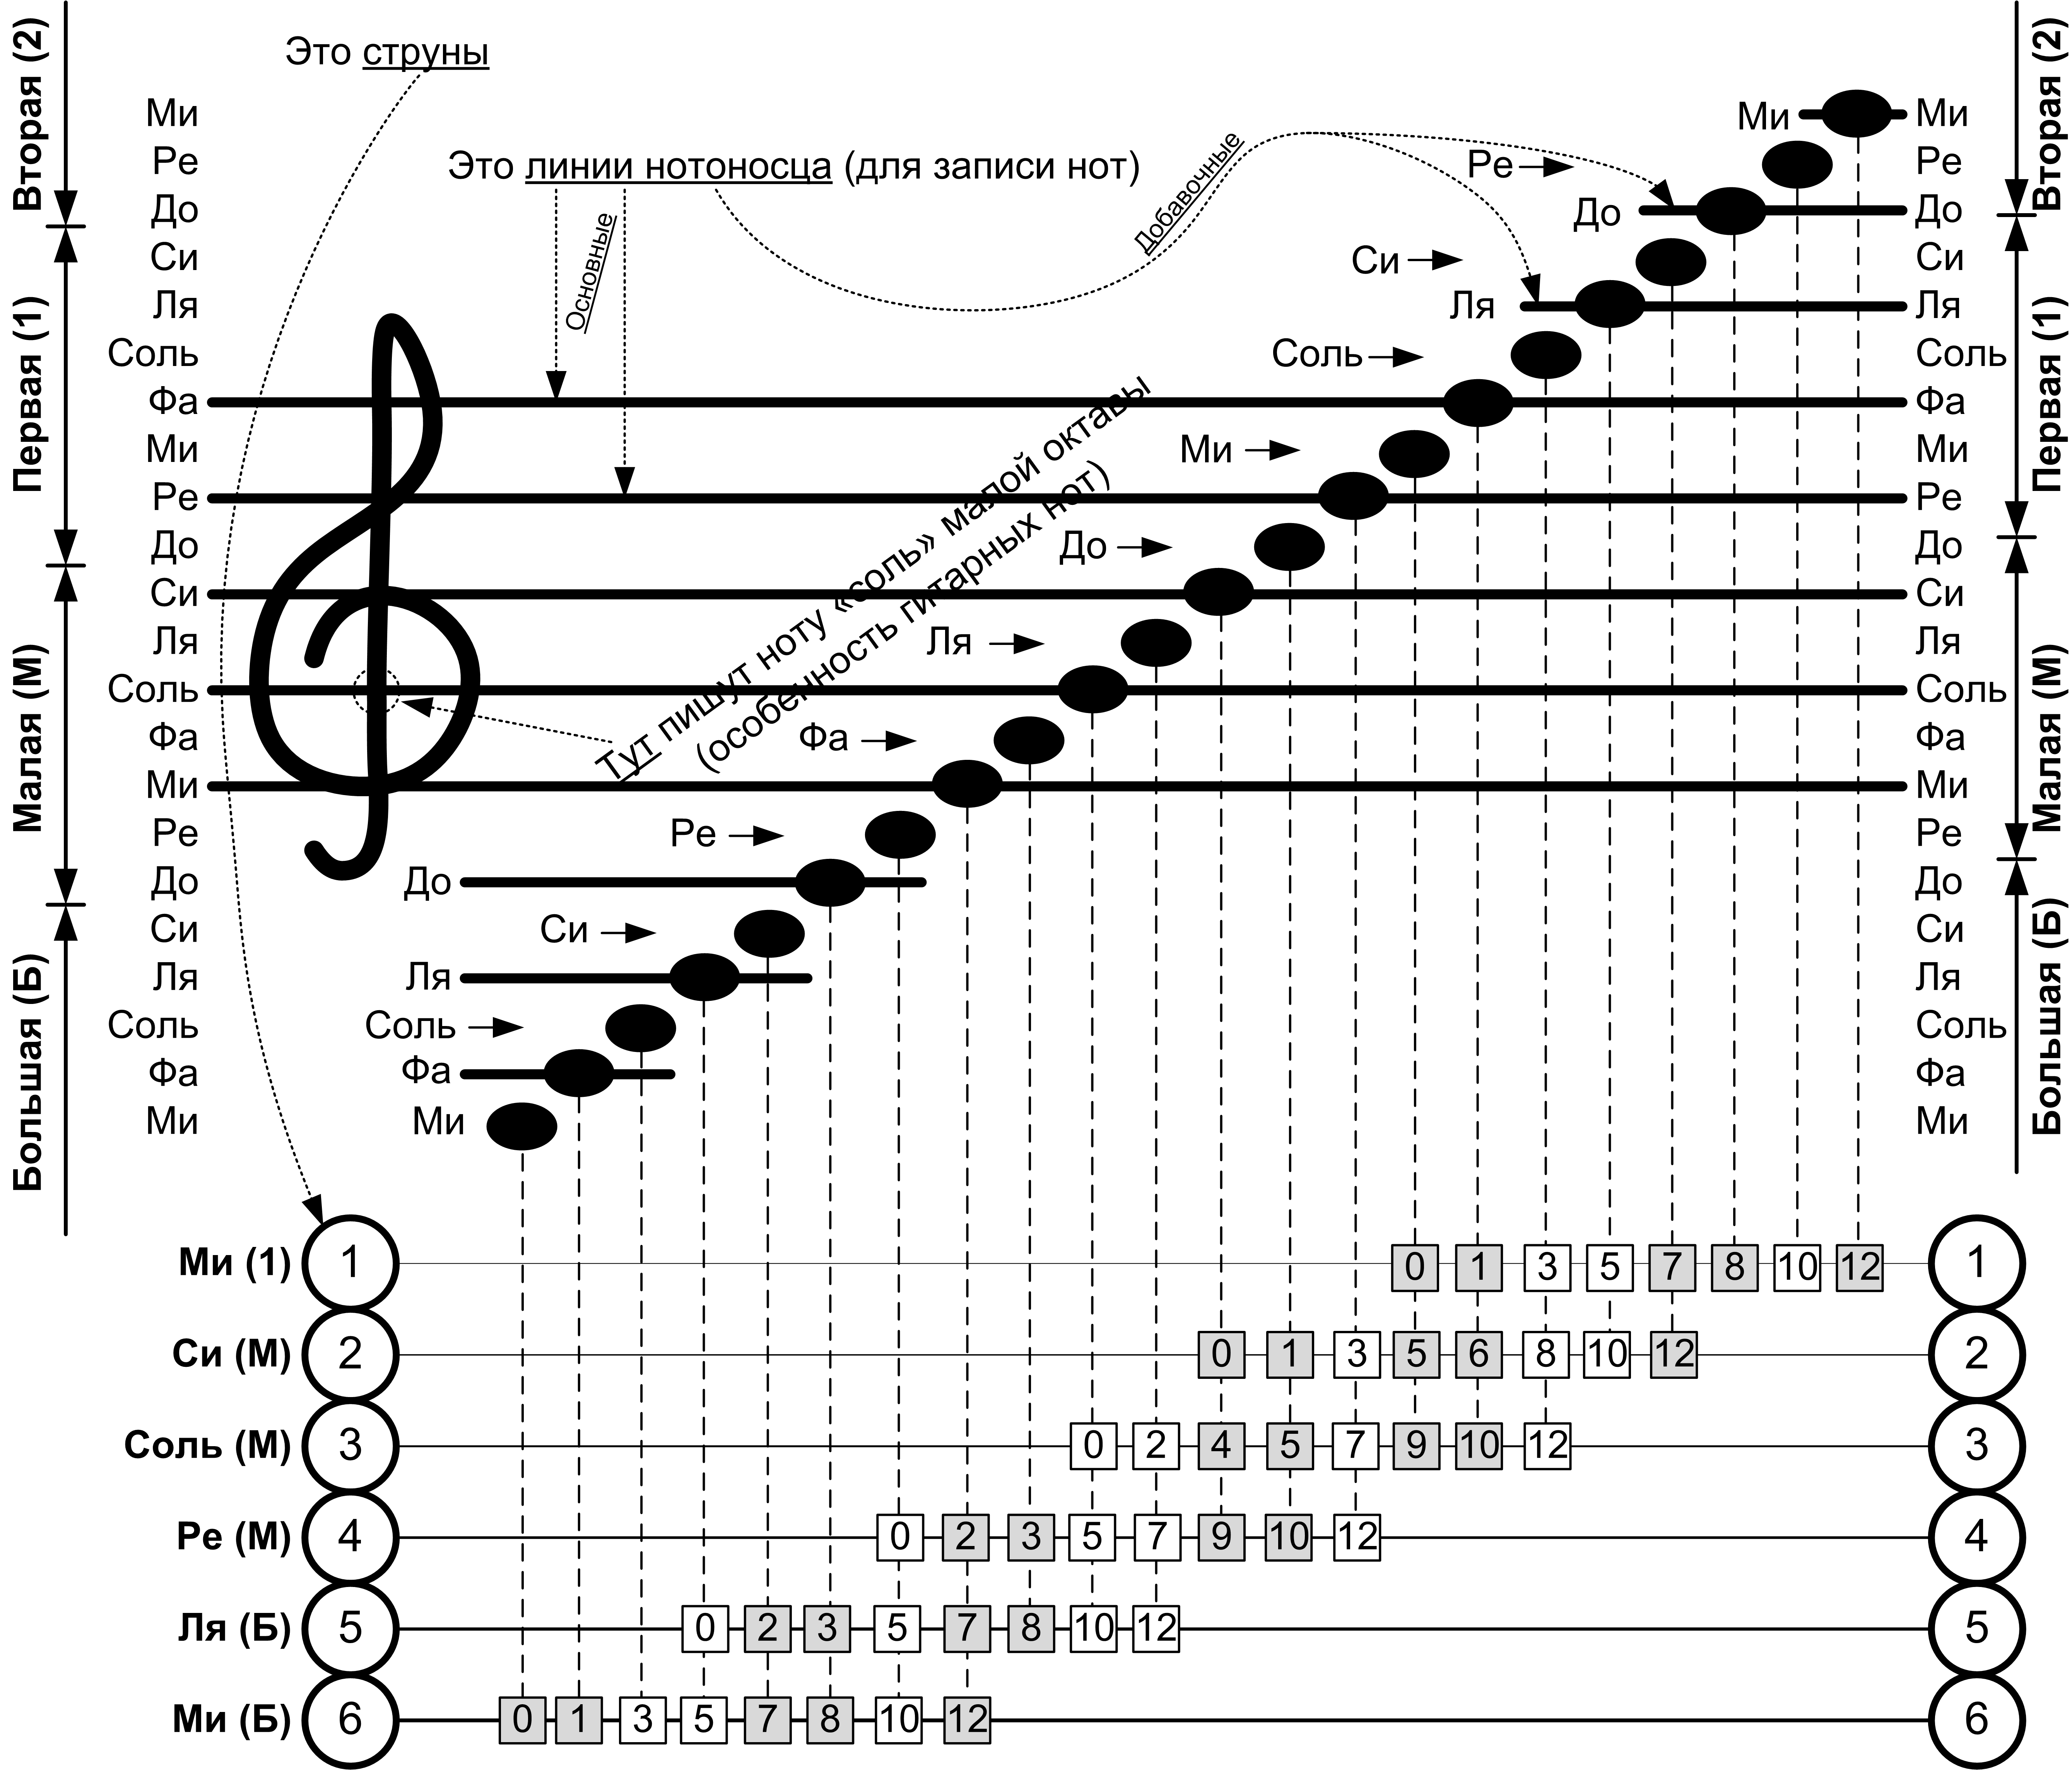
\includegraphics[width=\textwidth]{fig/lad-by-griph} 
    \caption{Ноты на грифе (гриф вдоль нотоносца)}\label{fig:ladByGriph}
\end{figure} 

\begin{figure}[!ht]
    \centering
    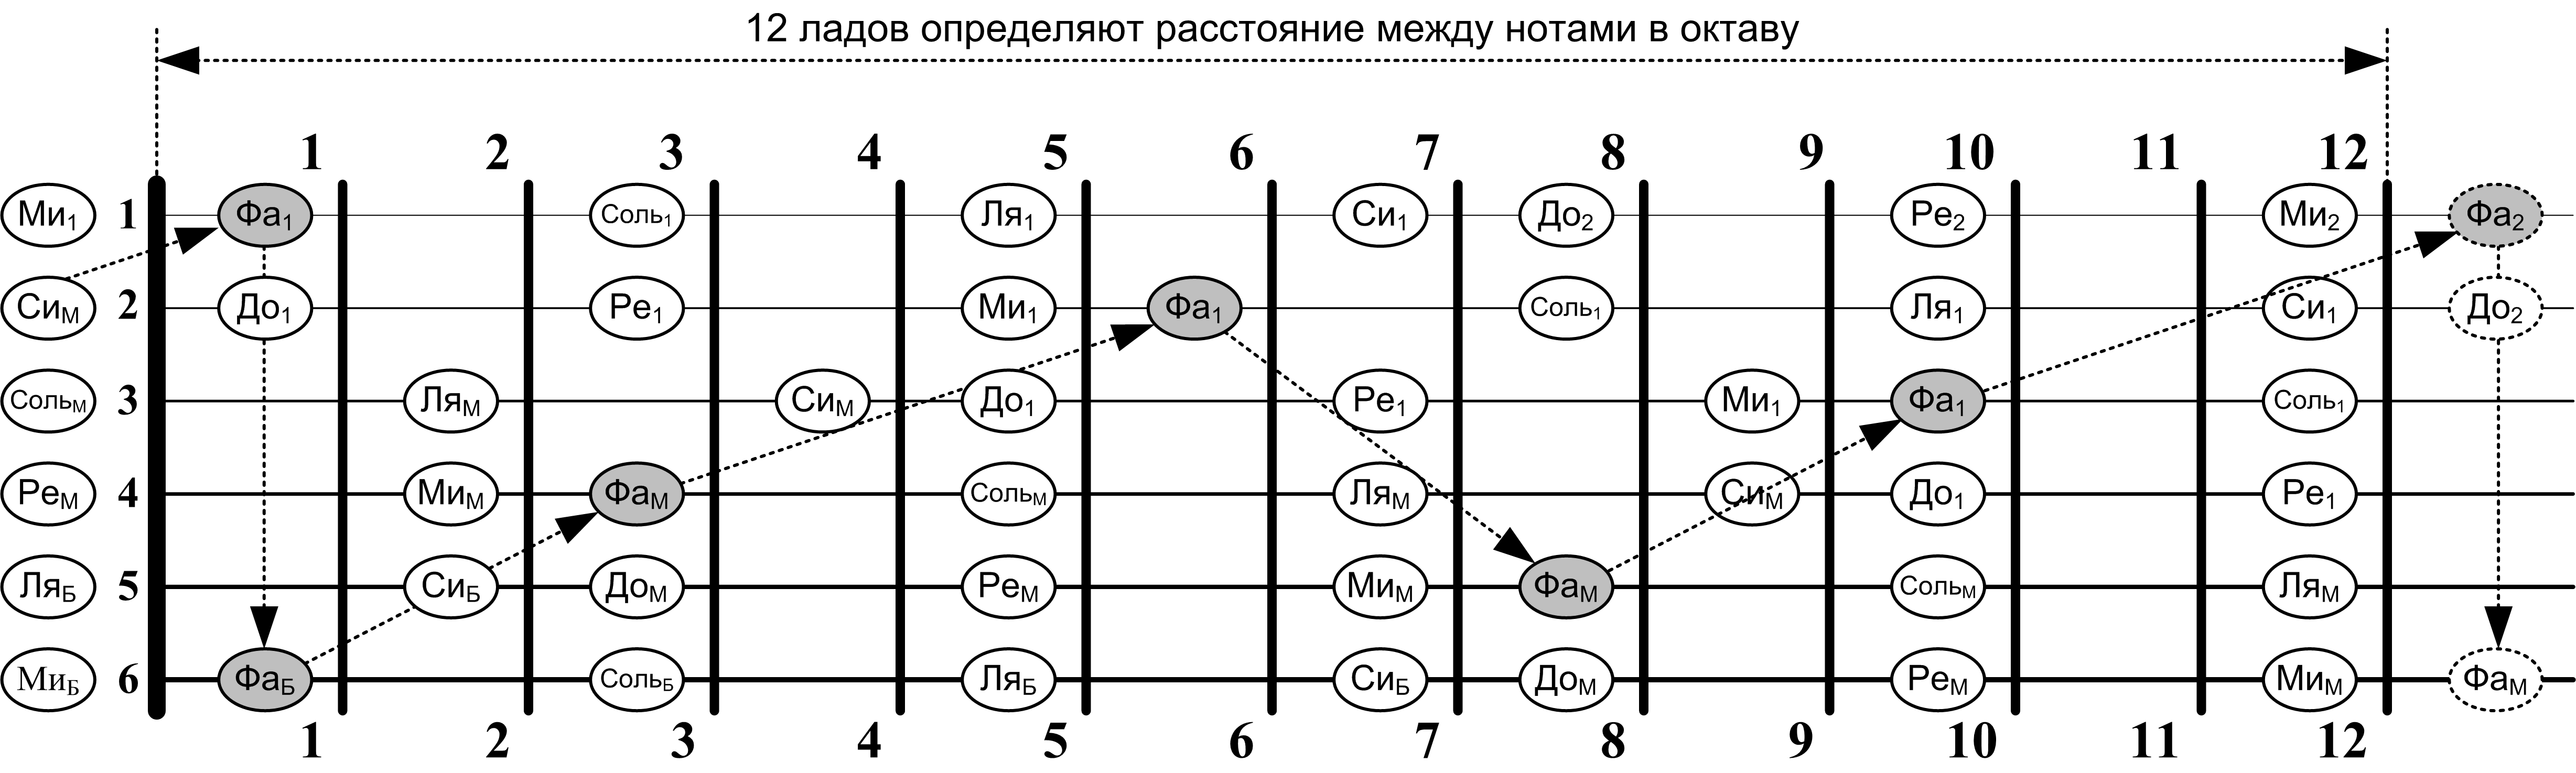
\includegraphics[width=\textwidth]{fig/notes-on-griph} 
    \caption{Ноты на грифе (относительное расположение)}\label{fig:notesOnGriph}
\end{figure} 


\section{Гитарная табулатура}

    %о нотной грамоте пару ласковых
    \chapter{А это что за штука? Устройство гитары}
\label{ch:guitar}

Частота от звука к звуку повышается в \emph{геометрической} прогрессии. То есть частота каждого следующего музыкального звука в \[\sqrt[12]{2}\approx 1,059463\] больше частоты звука предыдущего.

Так, следующий за ЛЯ первой октавы, звук ЛЯ-диез, имеет частоту $440\cdot\sqrt[12]{2}\approx 466,16$ герц. Звук СИ имеет частоту $440\cdot(\sqrt[12]{2})^2\approx 493,88$. И так далее, например, ЛЯ второй октавы имеет, как и положено, в два раза большую частоту, чем ЛЯ первой октавы: $440\cdot(\sqrt[12]{2})^{12}=440\cdot 2=880$ Гц.

Задав эталонную частоту любого музыкального звука, частоты для всех остальных звуков можно \emph{вычислить}.


TODO: ноты на грифе

\section{Может разберем? Конструкция}
\label{ch:guitar:construction}

Мы разобрались с теорией нот в предыдушем разделе, теперь коснемся особенностей устройства гитары, которые позволяют извлекать ноты именно такими, какими они и должны быть. 

Для начала стоит взглянуть на рисунок \ref{fig:guitar:construction} и запомнить, что значат незнакомые вам обозначения.

\begin{figure}[!ht]
    \centering
    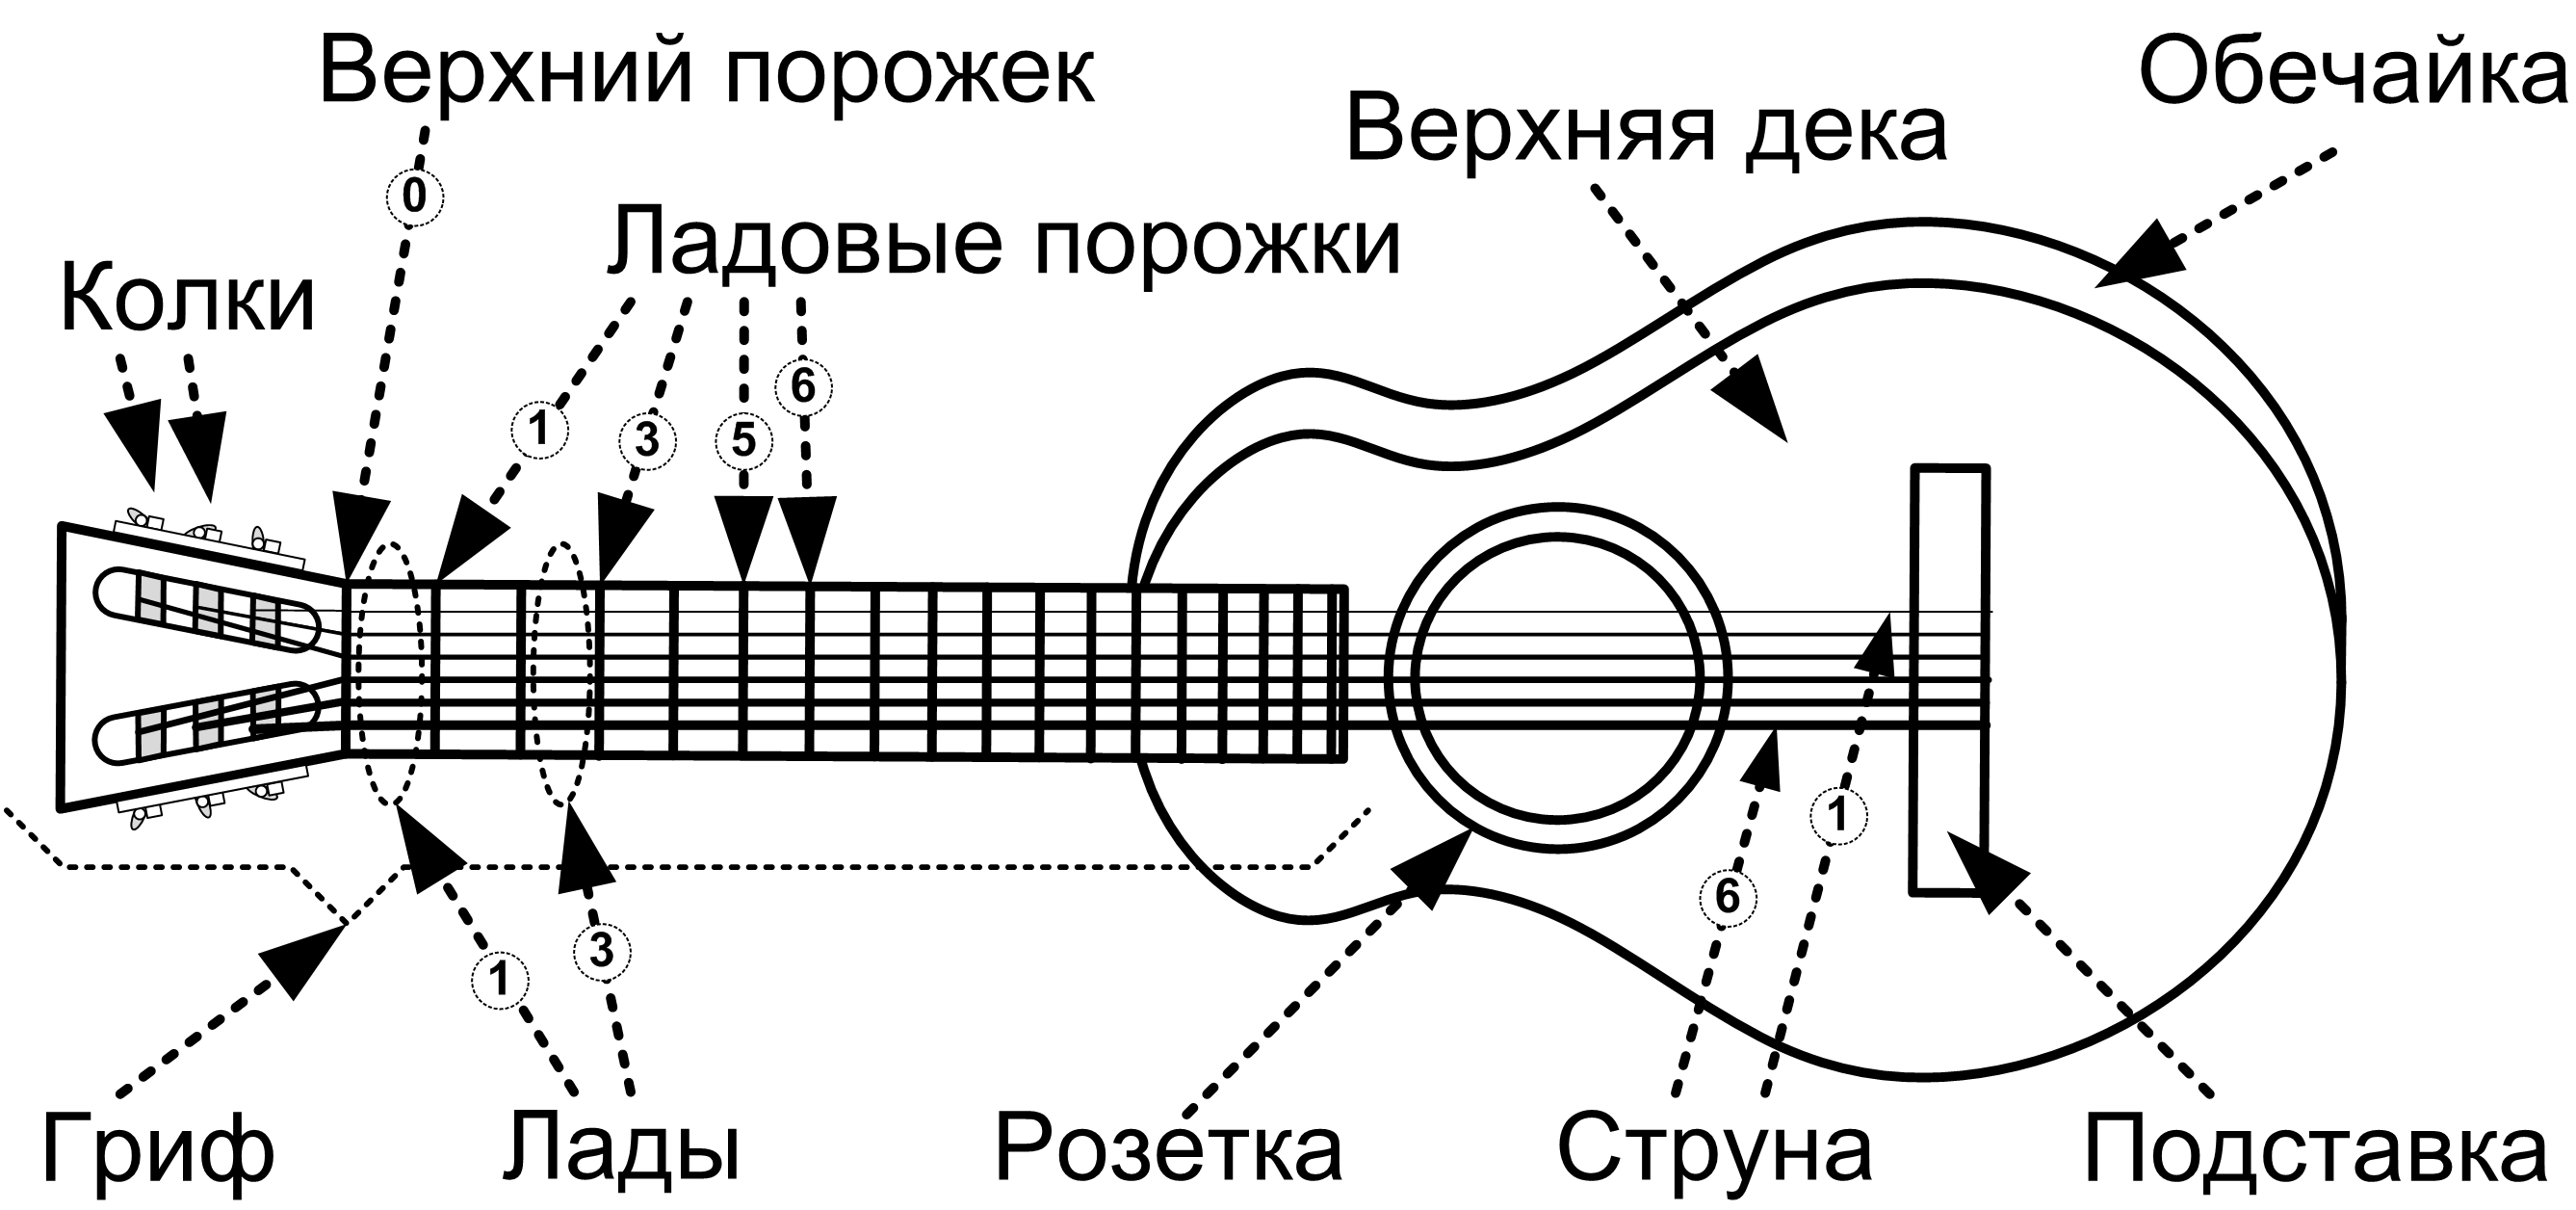
\includegraphics{fig/guitar-construction} 
    \caption{Устройство гитары}\label{fig:guitar:construction}
\end{figure} 

Любая открытая\footnote{То есть не зажатая ни на каком ладу} струна гитары звучит строго определенной нотой (о настройке гитары поговорим позже). Лады на грифе (промежутки между порожками), равно как и \emph{ладовые порожки} считаются от \emph{верхнего} порожка: 1,2,3,\ldots и т.д. То есть <<зажать струну на первом ладу>> значит, что вы ставите палец на струну, на первый лад, то есть между верхним порожком и первым ладовым\footnote{Чем ближе к первому ладовому, тем лучше. Таким образом и звук будет чище, и рука уставать будет меньше. Ставить палец сверху на порожек не стоит --- звук будет <<глохнуть>>. Правда иногда именно это и требуется. Но в начале обучения стоит ставить палец на ладу ближе к тому порожку, от которого идет <<звучащая>> часть струны. Добивайтесь чистого звука.} и нажимаете до тех пор, пока струна не прижмётся к первому ладовому порожку. Но нам важно сейчас не то, как правильно зажимать струну. 

Важно понять, что каждый следующий лад повышает звук на струне на <<полутон>>. В октаве 12 нот и каждая звучит на струне на своём ладу. На дветадцатом ладу звучит нота открытой струны, только выше на октаву.

Из физики известно, что частота колебаний струны обратно пропорциональна её длине\footnote{Надо честно заметить, что частота колебаний струны зависит также и от силы её натяжения, которая меняется, когда струну <<зажимают>> на ладу. Но это влияние столь незначительно, что им можно пренебречь.}. Стало быть, чтобы частота издаваемого струной звука \emph{увеличилась} вдвое (а языком музыки --- чтобы нота зазвучала октавой выше), надо вдвое \emph{укоротить} струну. 

Зажимая струну на 12 ладу (языком музыки --- повышая ноту открытой струны на октаву), вы укарачиваете звучащую часть струны вдвое. Линейка в помощь, если не верите\footnote{Конечно нужно мерять только звучащую (колеблющуюся часть) струны от опоры на подставке до 12-го ладового порожка.}.

Конечно, частота колебаний струны зависит также и от силы её натяжения. Сила натяжения струны регулируется колками на грифе, когда гитару настраивают. Играя, гитарист только меняет длину звучащего участка струны, зажимая струны на ладах. Редкие психи\footnote{Конечно, имелось в виду: \emph{мастера}! Прим. ред.} крутят колок во время исполнения, добиваясь сомнительных\footnote{Конечно, имелось в виду: \emph{удивительных}! Прим. ред.} эффектов.

Исходя из того, что частота каждой следующей ноты в $\sqrt[12]{2}$ больше предыдущей, запишем формулу длины струны ($L$) от места крепления струны к подставке до $n$-го ладового порожка:

\begin{equation}
    \label{fig:guitar:construction:length}
    L(n)=\frac{L}{(\sqrt[12]{2})^n},
\end{equation}

где $n$ - номер лада ($0$-й лад соответствует открытой струне), а $L$ --- общая длина струны от подставки до верхнего порожка.


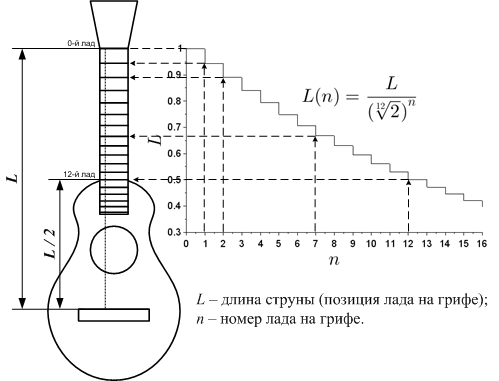
\includegraphics{fig/string-length.png}


Из картинки, надеюсь, ясно, почему ладовые порожки на гитаре расположены не на равном расстоянии друг от друга.

Кстати, некоторые ушастые выпендрёжники говорят, что различают своим сверхмузыкальным слухом больше 12 нот в октаве! И им мало 12 ладов! Есть спрос --- есть предложение: на некоторых гитарах можно заметить дополнительные ладовые порожки между <<каноническими>>, которые позволяют <<всунуть>> дополнительную ноту.


\section{Запись гитарных нот на бумаге}

Чтобы записать ноты, купите нотную тетрадь или на обычном листе начертите нотоносец --- пять параллельных, расположенных друг под другом через равные интервалы (около двух миллиметров) линий:
 

Традиционно ноты для шестиструнной гитаре записываются в скрипичном ключе, который своим хвостиком огибает вторую снизу линию нотоносца, на которой располагется СОЛЬ \emph{малой} октавы\footnote{Для других музыкальных инструментов, в первую очередь, для фортепиано, скрипичный ключ показывает положение СОЛЬ \emph{первой} октавы, но для гитары, чтобы использовать один нотоносец, ноты пишут на <<фортепианный>> скрипичный нотоносец на октаву выше.}.


\section{Поиск нот на грифе}

\begin{figure}[!ht]
    \centering
    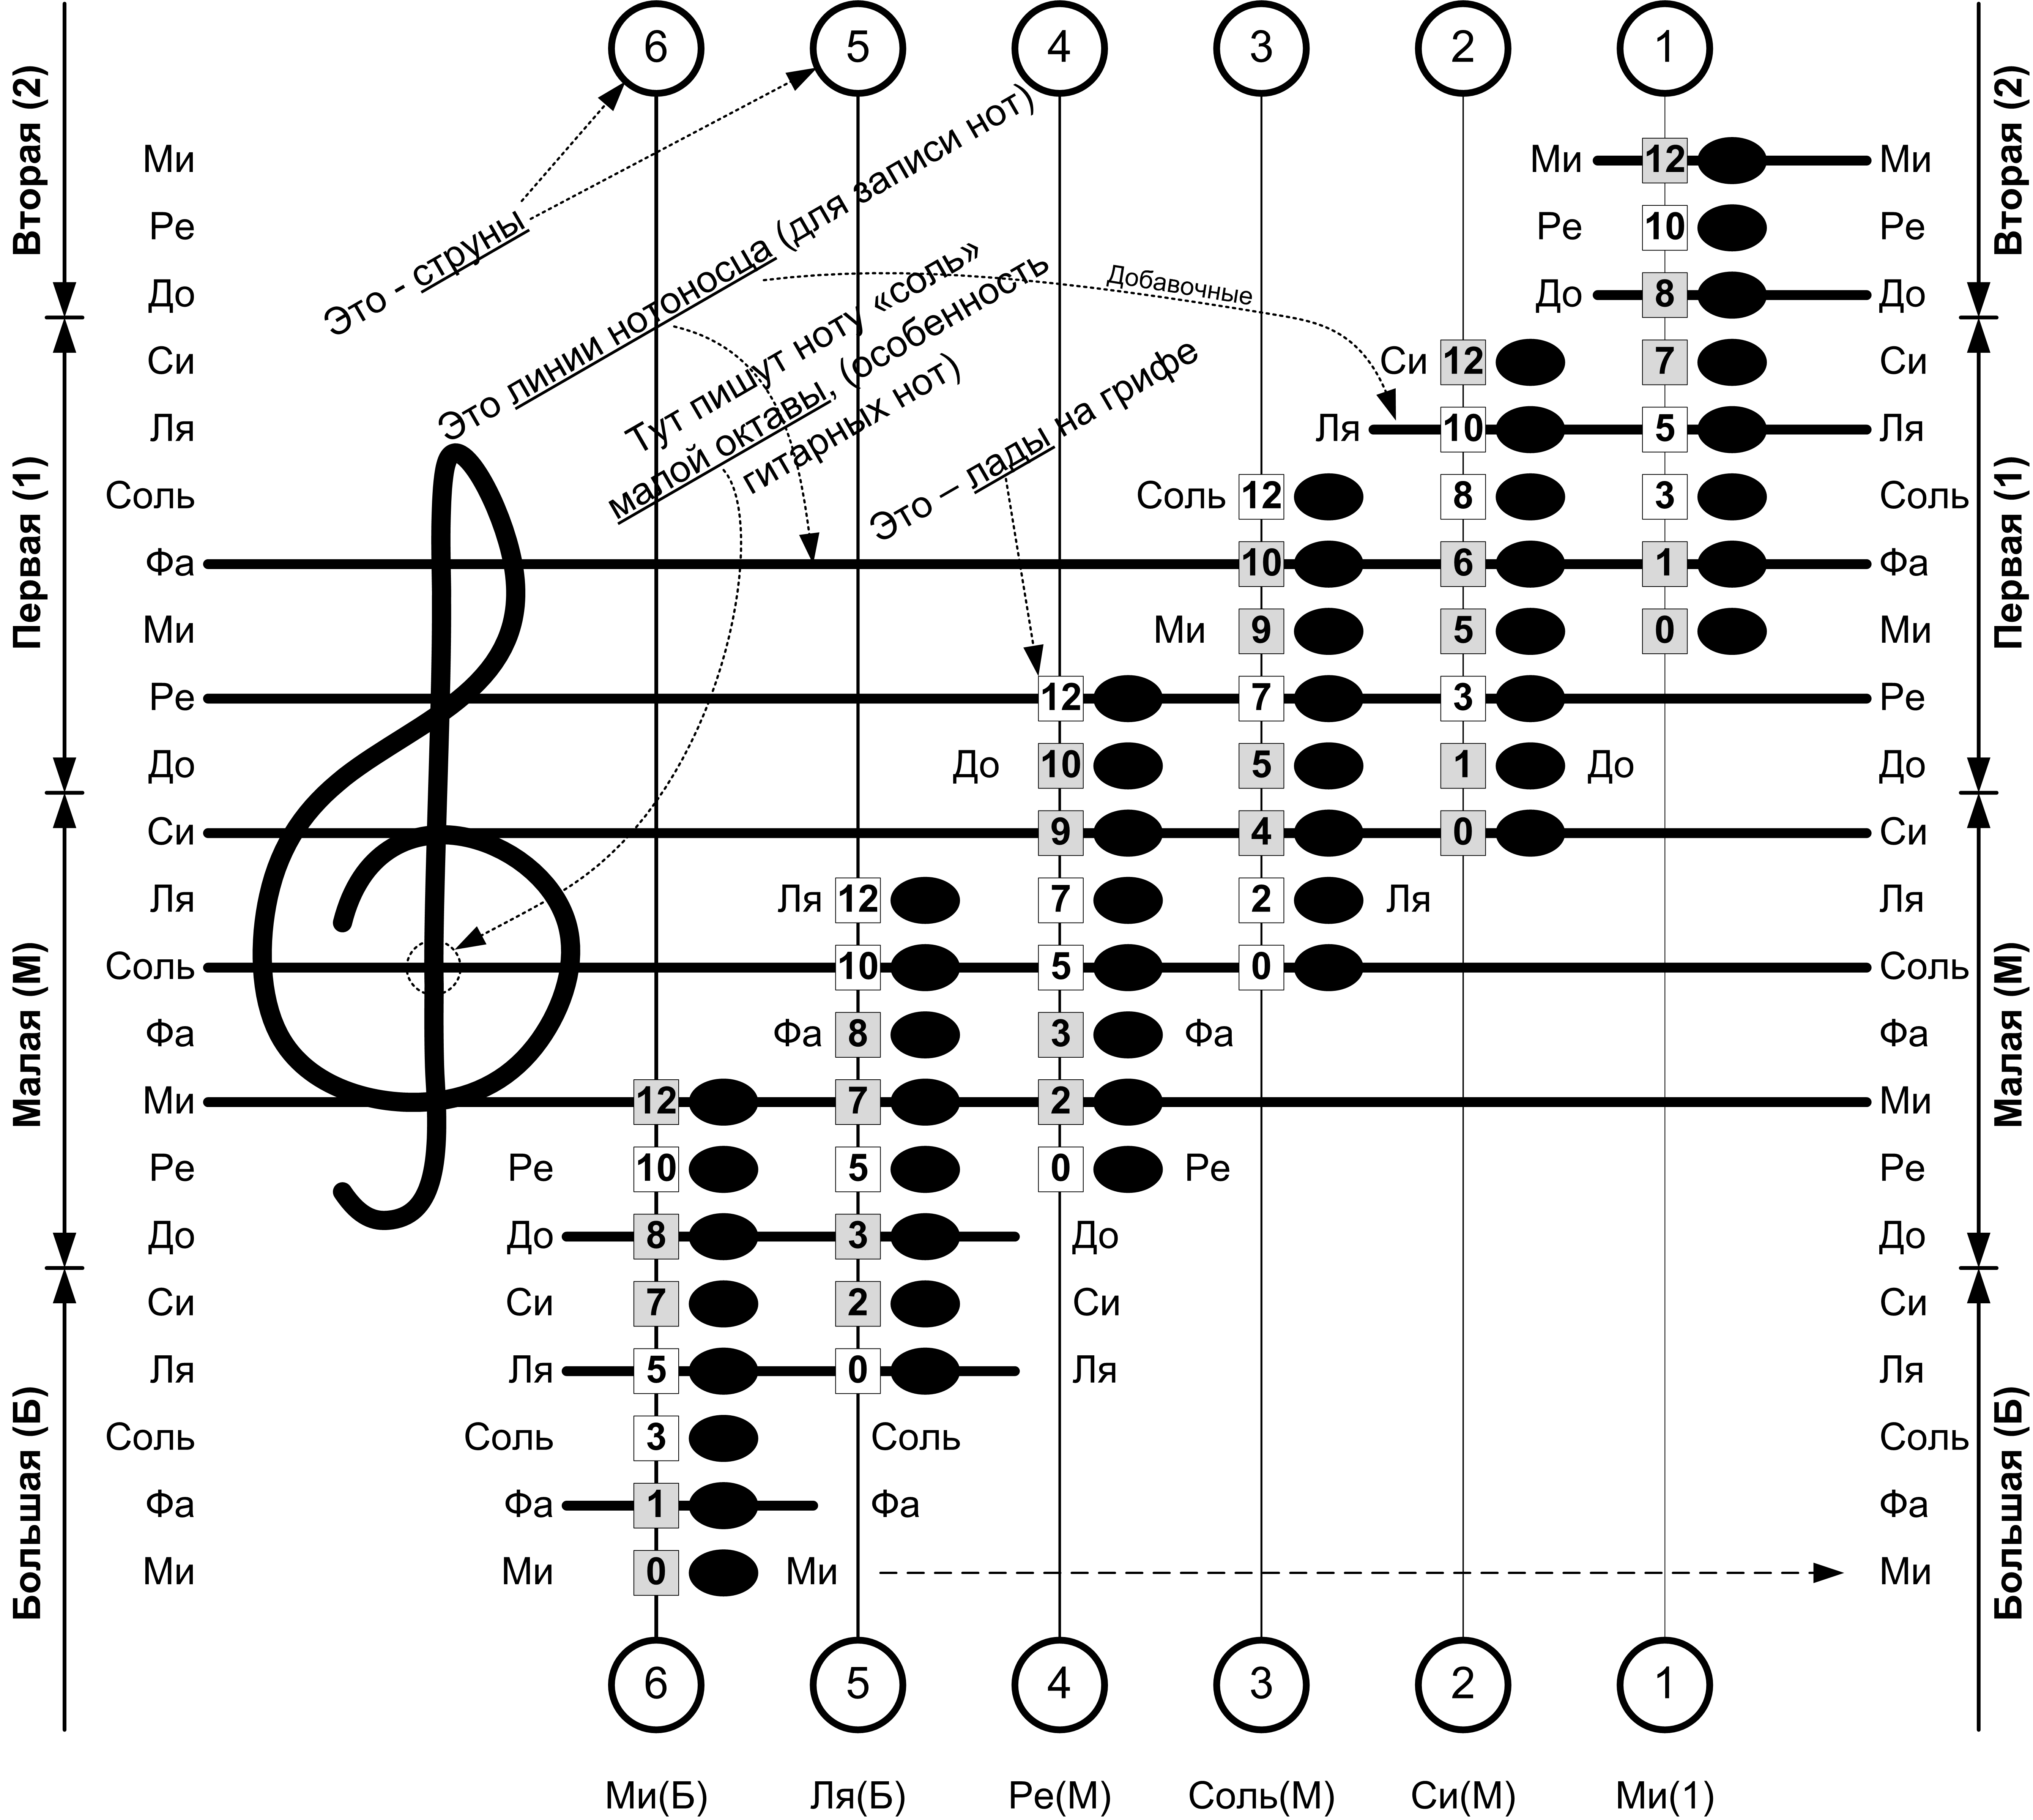
\includegraphics[width=\textwidth]{fig/lad-by-notes} 
    \caption{Ноты на грифе (гриф поперек нотоносца)}\label{fig:ladByNotes}
\end{figure} 

\begin{figure}[!ht]
    \centering
    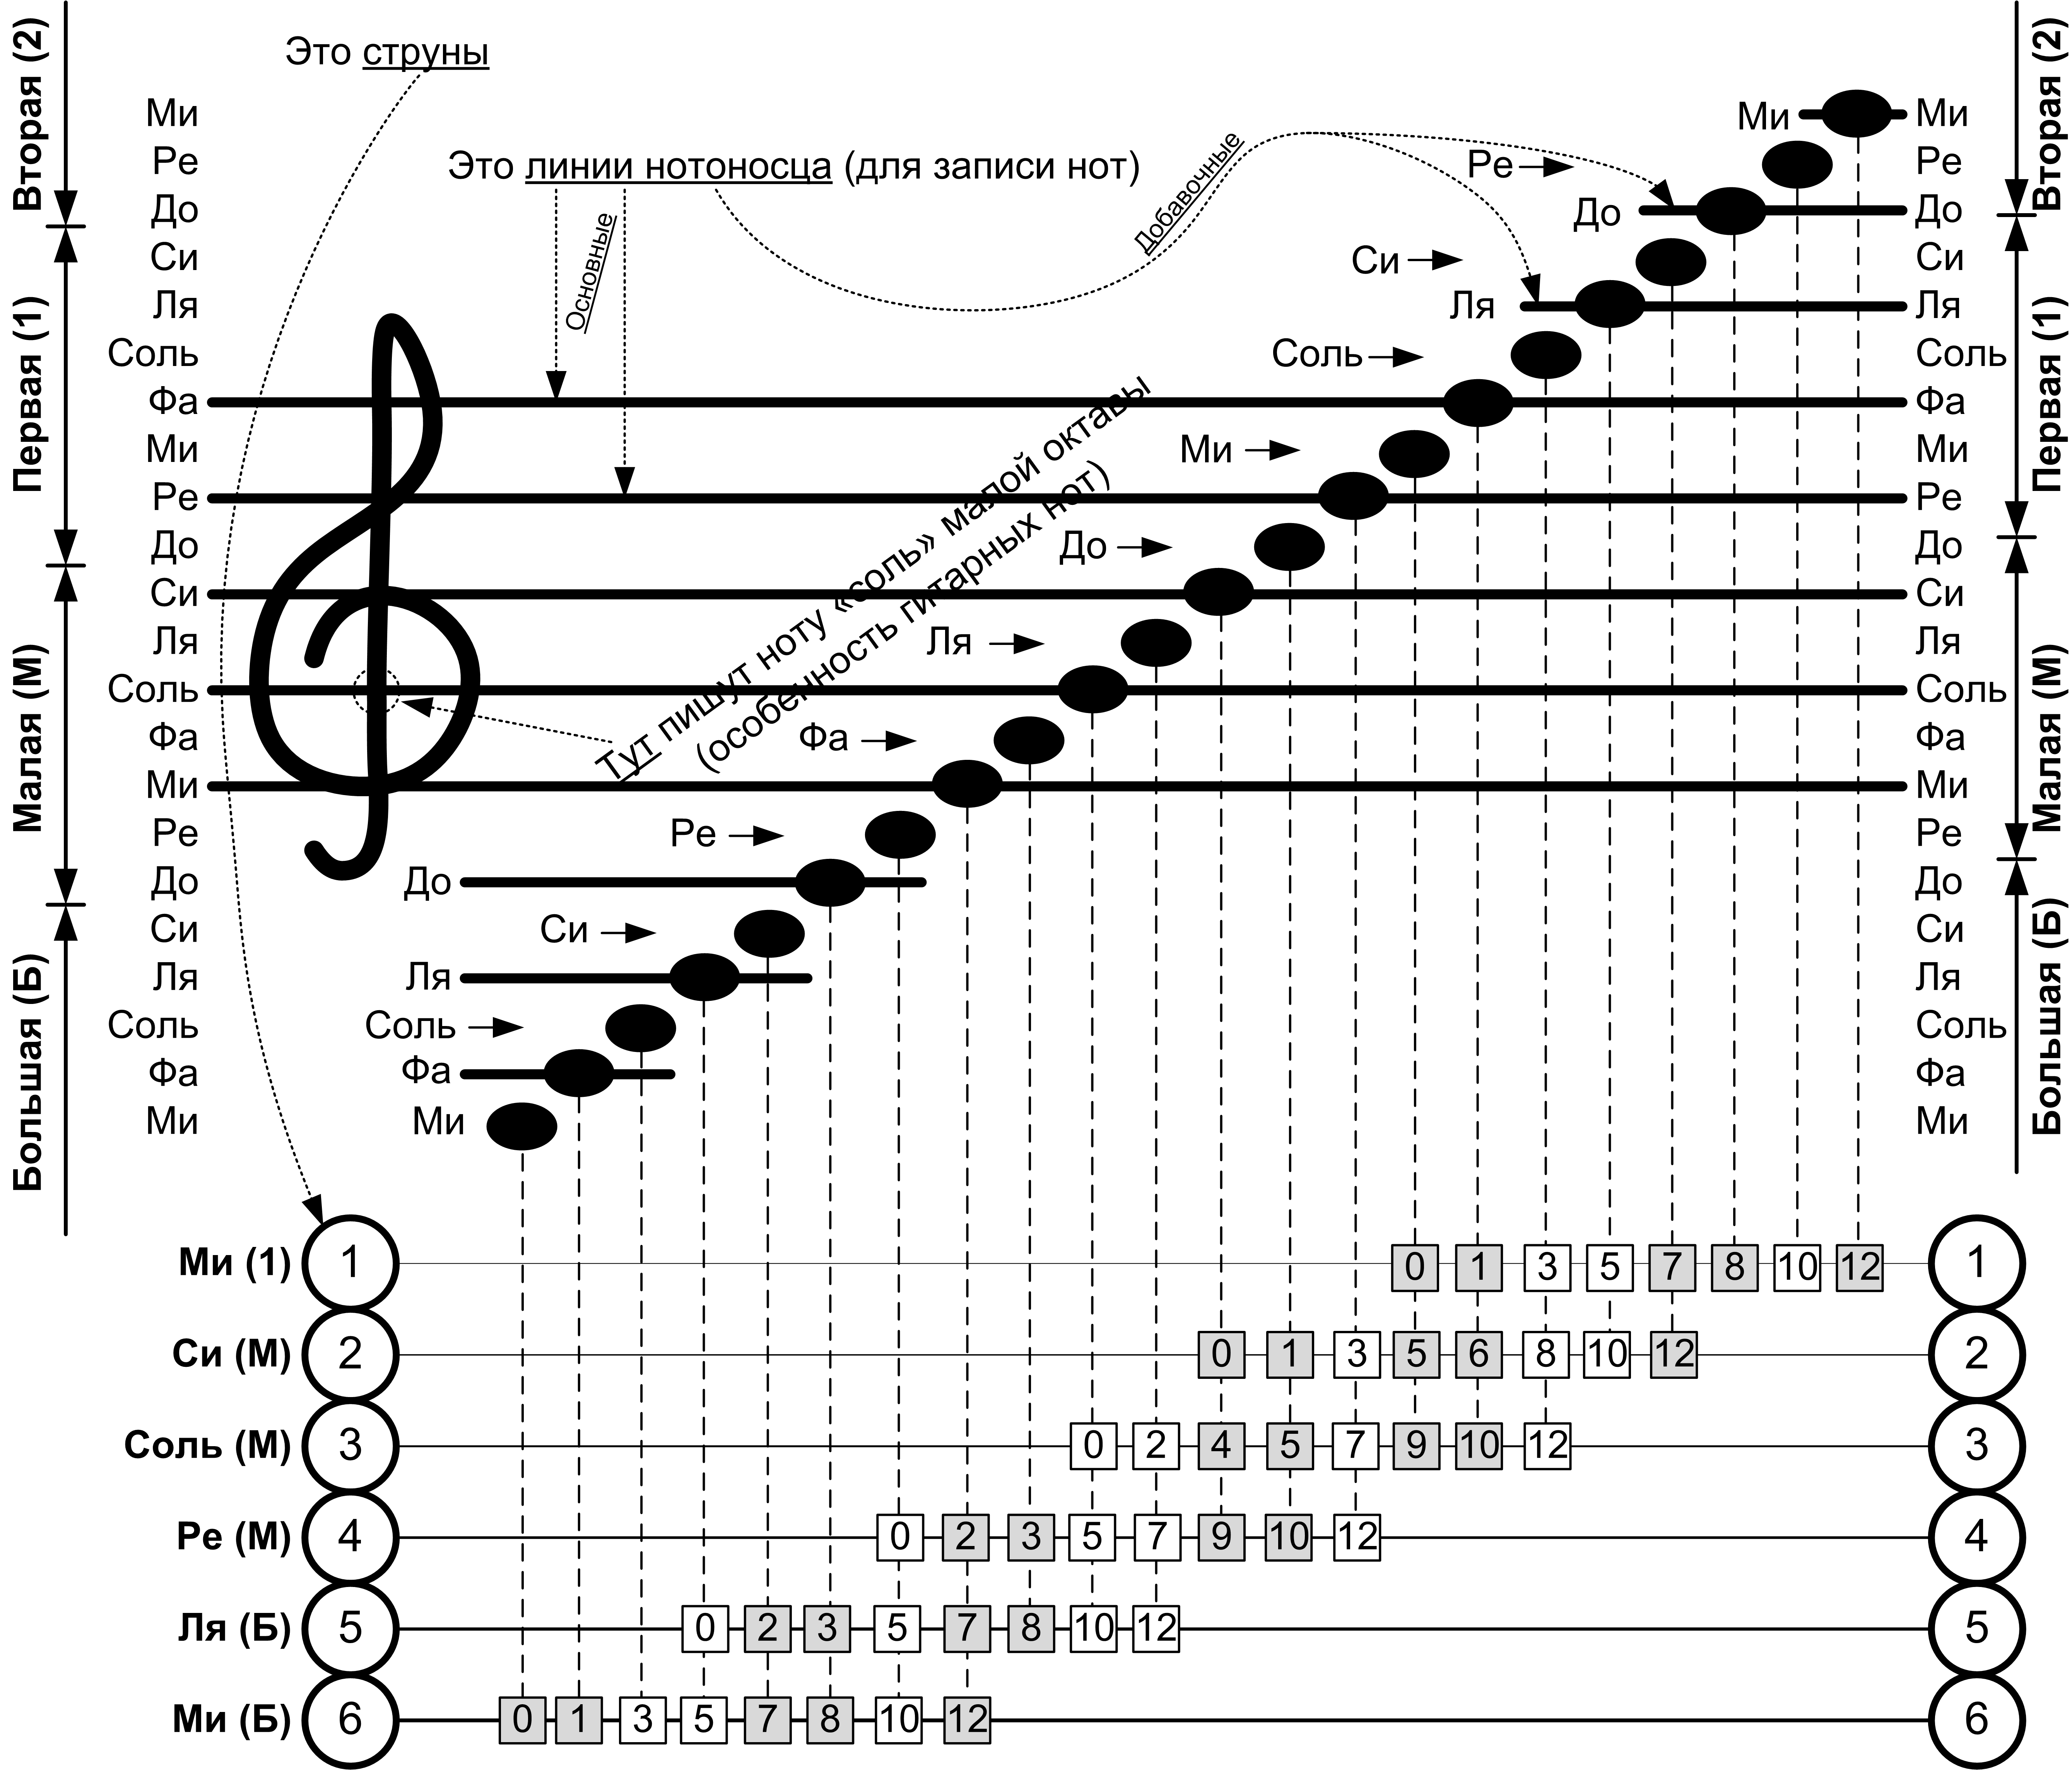
\includegraphics[width=\textwidth]{fig/lad-by-griph} 
    \caption{Ноты на грифе (гриф вдоль нотоносца)}\label{fig:ladByGriph}
\end{figure} 

\begin{figure}[!ht]
    \centering
    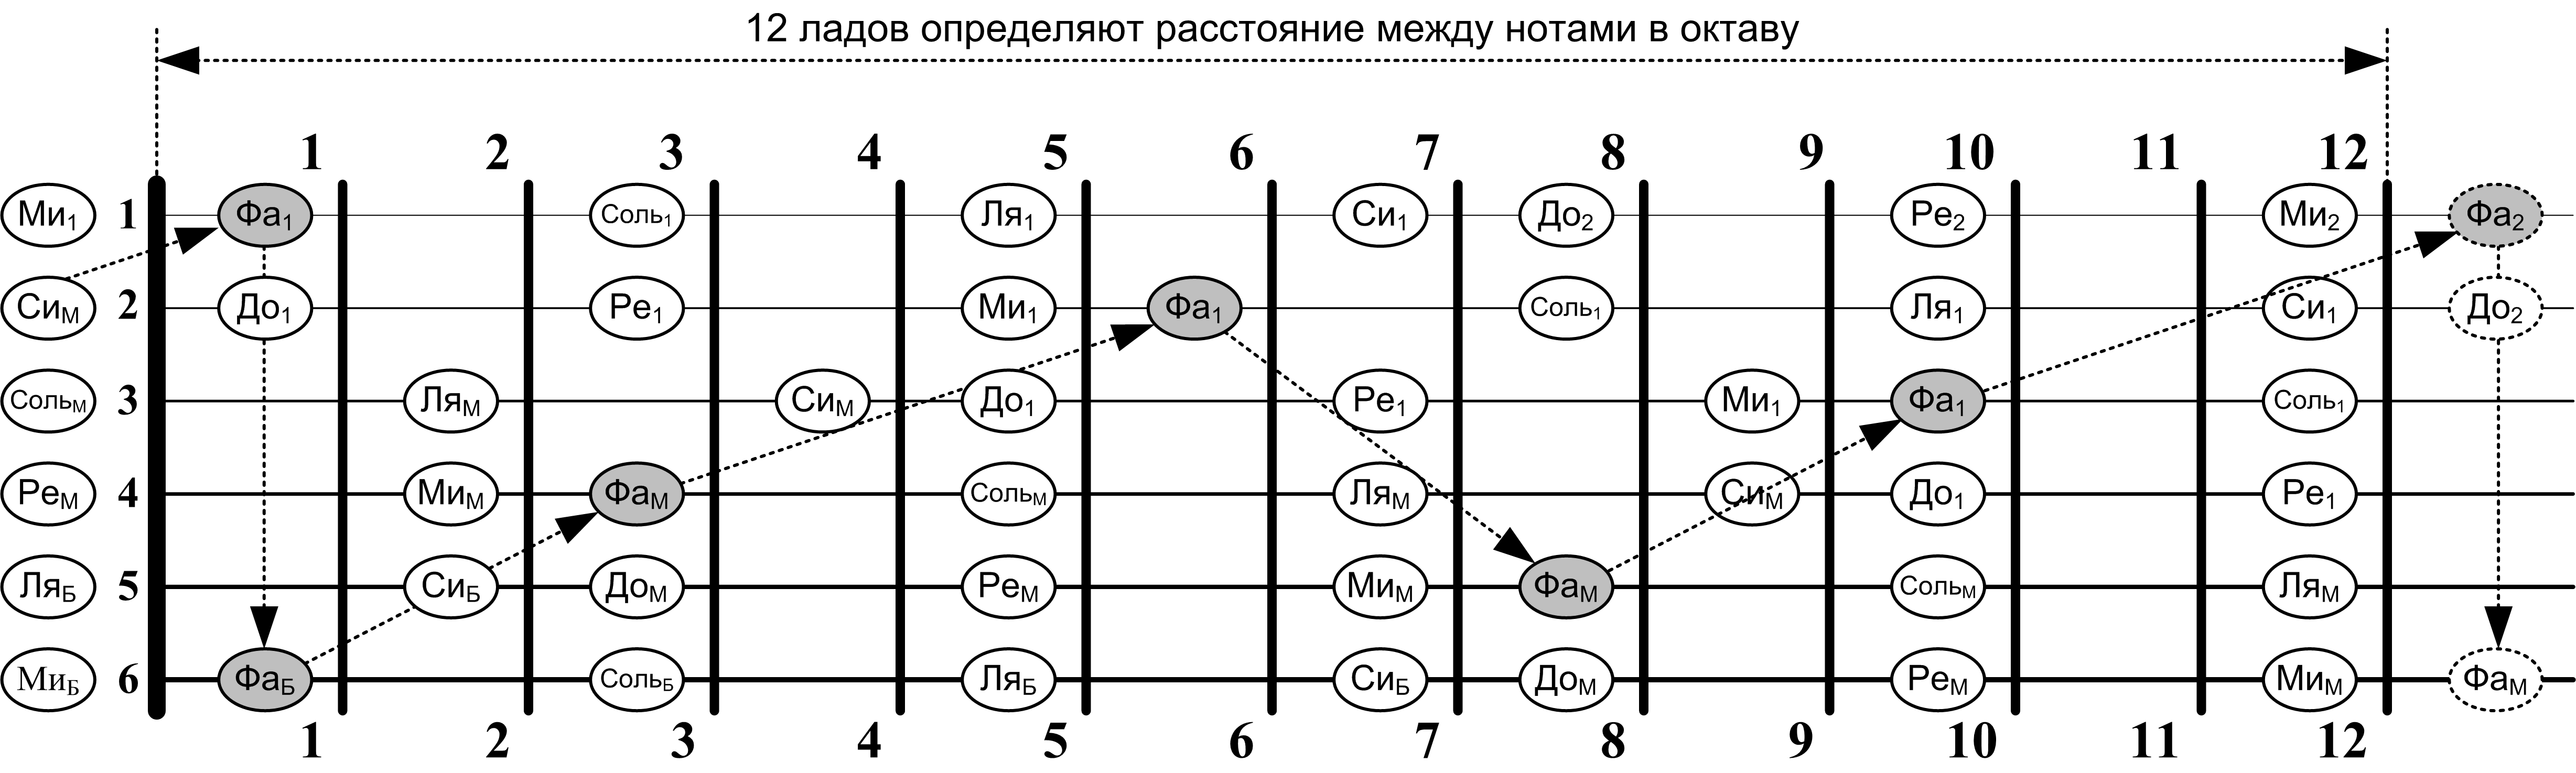
\includegraphics[width=\textwidth]{fig/notes-on-griph} 
    \caption{Ноты на грифе (относительное расположение)}\label{fig:notesOnGriph}
\end{figure} 


   %об устройтсве гитары
    \chapter{А так звучит красиво? Гармоничность}
\label{ch:harmony}


Подчинаяется наше восприятие музыки каким-либо законам? Безусловно.

Что же тогда определяет наши вкусы\index{гармония}:
\begin{itemize}
    \item математика и физика;
    \item сформировавшиеся за многие годы общие культурные привычки;
    \item индивидуальные особенности;
    \item что-то еще?
\end{itemize}

По порядку.
\begin{itemize}
    \item Как уже было сказано --- математика внутри нас, а физика --- снаружи. Так что существуют универсальные формальные законы, определяющие <<что такое \emph{хорошо} и что такое \emph{плохо}>>.
    \item Наши предки нашли и оставили нам много законов гармонии, в соответствии с которыми писалась музыка и формировались наши музыкальные вкусы. И многое из того, что нам нравится --- результат привычки, корни которой прорастают вглубь поколений.
    \item Восприятие окружающего мира индивидуально. Хоть каждый из нас укомплектован сходным набором сенсовров: зрительных, слуховых, обонятельных, вкусовых, осязательных, гравитационных и, возможно, каких-то ещё, но вряд ли вы найдете двух людей с абсолютно, до молекулы, идентичными сенсорами. А уж об идентичности сформировавшихся нейронных связей можно даже не мечтать. Как говорится: <<на вкус и цвет товарищей нет>>. И тут математики должны внести ясность: это на малой выборке (например, семья или круг близких друзей) товарищей нет, а на большой (стадион беснующихся фанатов) --- ещё как есть!
    \item Что-то ещё? Да, всегда есть загадочное и непознанное что-то ещё.
\end{itemize}


\section{Сколько вешать в полутонах? Интервалы}
\label{ch:harmony:interval}

\begin{Definition}[Интервал]
    \emph{Интервал}\index{интервал} --- это расстояние по высоте между \emph{двумя} музыкальными звуками, выраженное в полутонах. 
\end{Definition}

Это определение для математиков. Для музыкантов интервалы \emph{звучат}! Если два звука прозвучали одновременно, то интервал называется \emph{гармоническим}\index{интервал!гармонический}, а если друг за другом --- \emph{мелодическим}\index{интервал!мелодический}.

\begin{Example}[Послушаем гармонические интервалы]
    \label{ex:harmony:interval:string5and6}
    Возьмите настроенную гитару. Поиграем на 5 и 6-й струне. Если гитара настроена страндартно, то 6-я струна на 5-м ладу прозвучит в унисон с открытой 5-й струной. Такое расстояние в 0 полутонов музыканты называют \emph{примой}. 
    
    Инструмент обязательно должен быть настроен! Иначе эксперимент не получится.
    
    Теперь расслабьтесь, успокойтесь, забудьте обо всех горестях и радостях. Сосредоточьтесь на своём дыхании. Существует только ваше дыхание. Абсолютный покой. 
    
    Не получается? Ну и чёрт с ним!

    Вам нужно будет оценить свои ощущения от сыгранных интервалов. Поставьте каждому интервалу оценку, например по 5-и балльной шкале: 1(ужас), 2(срам), 3(терпимо), 4(хорошо), 5(прекрасно).
    
    Начнем. Зажмите 6-ю струну на 5-м ладу и одновременно сыграйте две струны: 6-ю и 5-ю. Звучит гармонический интервал \emph{прима}! Интервал в ноль полутонов. Прислушиваемся к ощущениям, ставим приме оценку.
    
    Продолжаем оценивать интервалы. Играем одновременно 5-ю открытую струну и 6-ю струну на 6-м ладу. Расстояние в 1 полутон. Оценивайте результат.
    
    И так далее, играем интервал в 2 полутона (6-я струна на 7-м ладу) и так далее до интервала в 12 полутонов (6-я струна на 17 ладу). 
    
    Читая этот раздел, периодически поглядывайте на получившиеся записи. Будет полезно.
\end{Example}

Интервал --- это настолько важное понятие в музыке, что каждое его числовое значение получило собственное имя. Например, интервал в 7 полутонов называется \emph{квинта}\index{интервал!квинта}. Мы будем оперировать с числами, но при первом упоминании я буду приводить сложившиеся названия интервалов в скобках, например <<7(\myNemph{квинта})>>, а чуть позже объясню, почему значения интервалов называются именно так.

Приятный на слух интервал (неважно, гармонический или мелодический) музыканты называют \emph{консонансом}\index{консонанс}, а неприятный --- \emph{диссонансом}\index{диссонанс}. 

Чтобы глубже разобраться в том, почему звучание одного интервала нам нравится, а другого --- нет, визуализируем результат наложения двух звуков. Пусть функция $\sin(x)$\index{синус функция} изображает колебания основного тона исходного звука. Функция $\sin(x\cdot(\sqrt[12]{2})^n)$ будет изображать звук, который \emph{выше} исходного на $n$ \emph{полутонов}. Результату совместного звучания (то есть гармоническому интервалу) будет соответствовать их сумма\footnote{В Интернете масса сайтов, позволяющих построить график функции. Более того, просто наберите в поисковой строке Google \texttt{sin(x)+sin(x*(2\^{}(1/12)))} и дивитесь чудесам Технологии!}:

\begin{equation}
    \label{eq:harmony:interval:sin}
    \sin(x) + \sin(x\cdot(\sqrt[12]{2})^n).
\end{equation}

Результаты построения графиков совместного звучания (построен красным цветом) на фоне исходного звука (синий цвет) для интервалов от $n=1$ до $n=11$ полутонов (т.е. в рамках октавы) приведены в таблицах \ref{t:harmony:interval:disso-1-2-10-11}, \ref{t:harmony:interval:conso-3-4-8-9}, \ref{t:harmony:interval:conso-5-7}, \ref{t:harmony:interval:disso-6}.

Диссонансы приведены в таблицах \ref{t:harmony:interval:disso-1-2-10-11} и \ref{t:harmony:interval:disso-6}. Диссонансы получаются на интервалах в 1(\myNemph{малая секунда}), 2(\myNemph{большая секунда}\index{интервал!секунда}), 6(\myNemph{увеличенная кварта}), 10(\myNemph{малая септима}) или 11(\myNemph{большая септима}\index{интервал!септима}) полутонов. Значит вам не должны были понравиться интервалы на 6, 7, 11, 15, 16 ладах 6-й струны, если вы обратили внимание на пример \ref{ex:harmony:interval:string5and6}. Что, неужели понравились?! Пора сходить к доктору или настроить гитару. Не затягивайте!

\begin{table}[!ht]
    \caption{Интервалы-диссонансы в графиках \eqref{eq:harmony:interval:sin}}
    \label{t:harmony:interval:disso-1-2-10-11}
    \centering
    \begin{tabular}{c|c}
        \hline\hline
        1 полутон, $n=1$        & 2 полутона, $n=2$ \\
        малая секунда           & большая секунда \\
        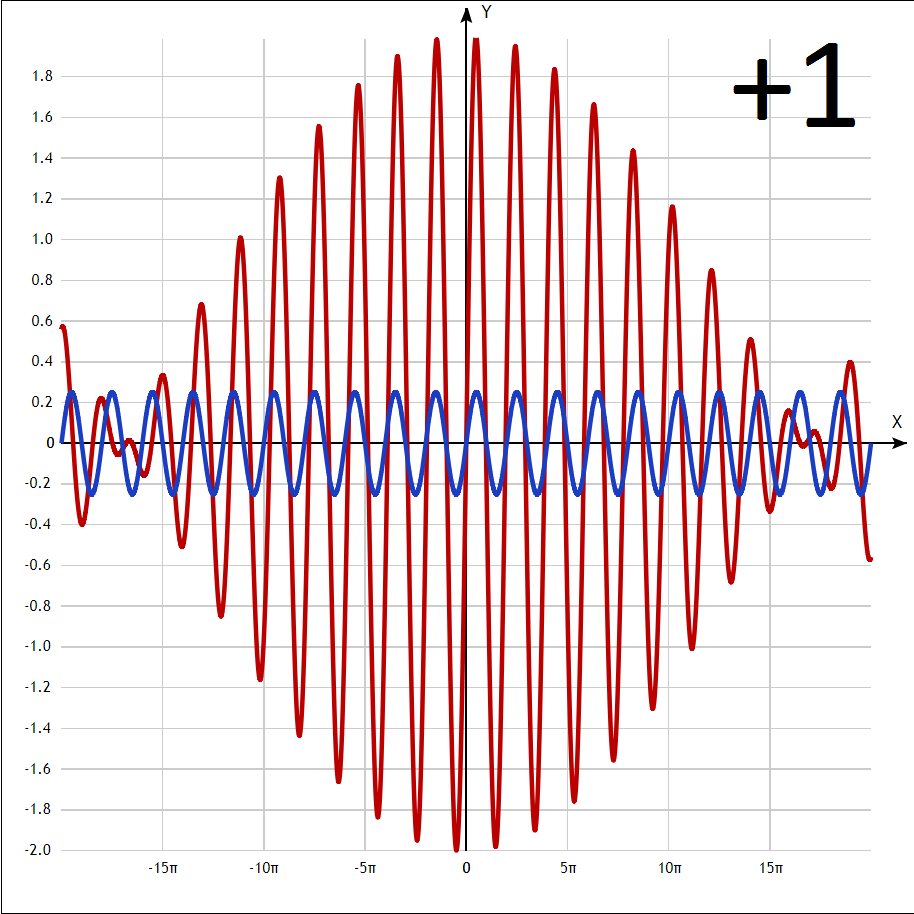
\includegraphics[width=0.45\textwidth]{fig/intervals/i01}
            & 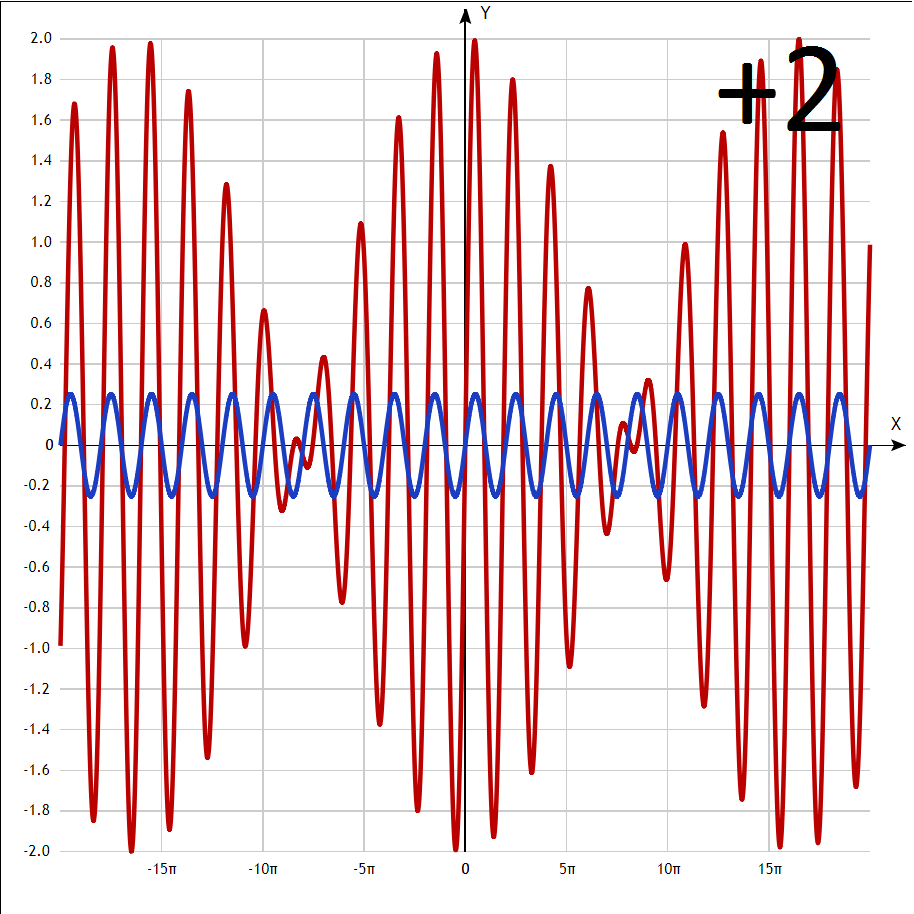
\includegraphics[width=0.45\textwidth]{fig/intervals/i02} \\
        \hline\hline
        10 полутонов, $n=10$    & 11 полутонов, $n=11$ \\
        малая септима           & большая септима \\
        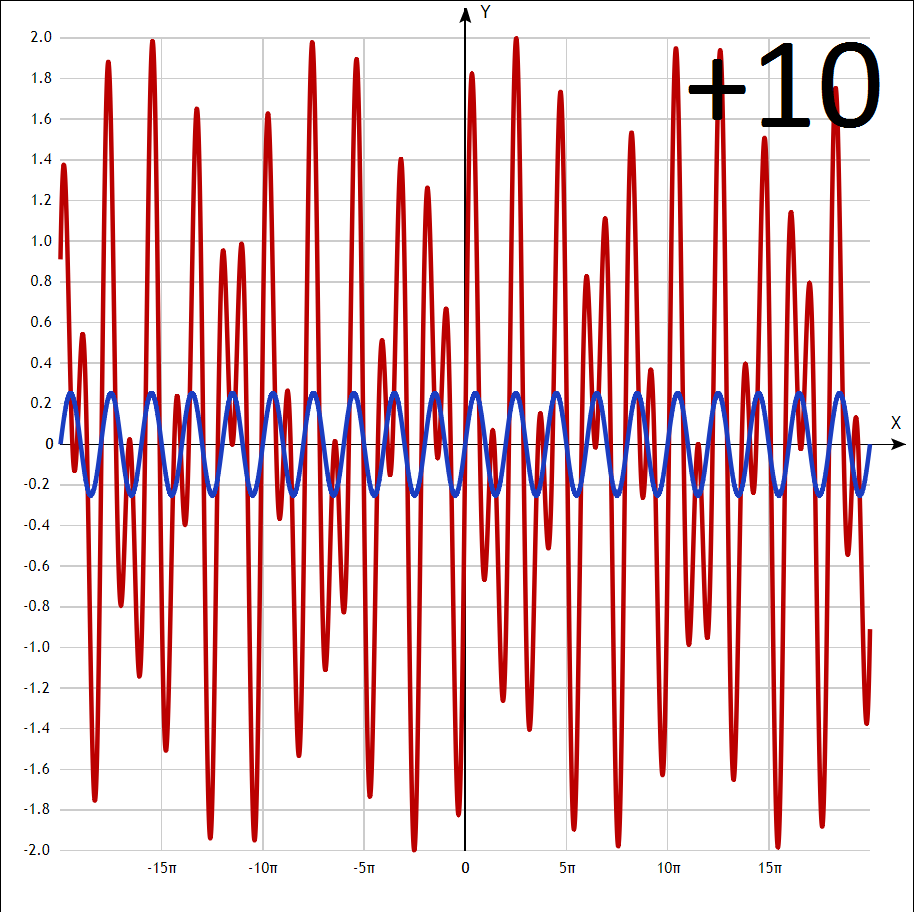
\includegraphics[width=0.45\textwidth]{fig/intervals/i10}
            & 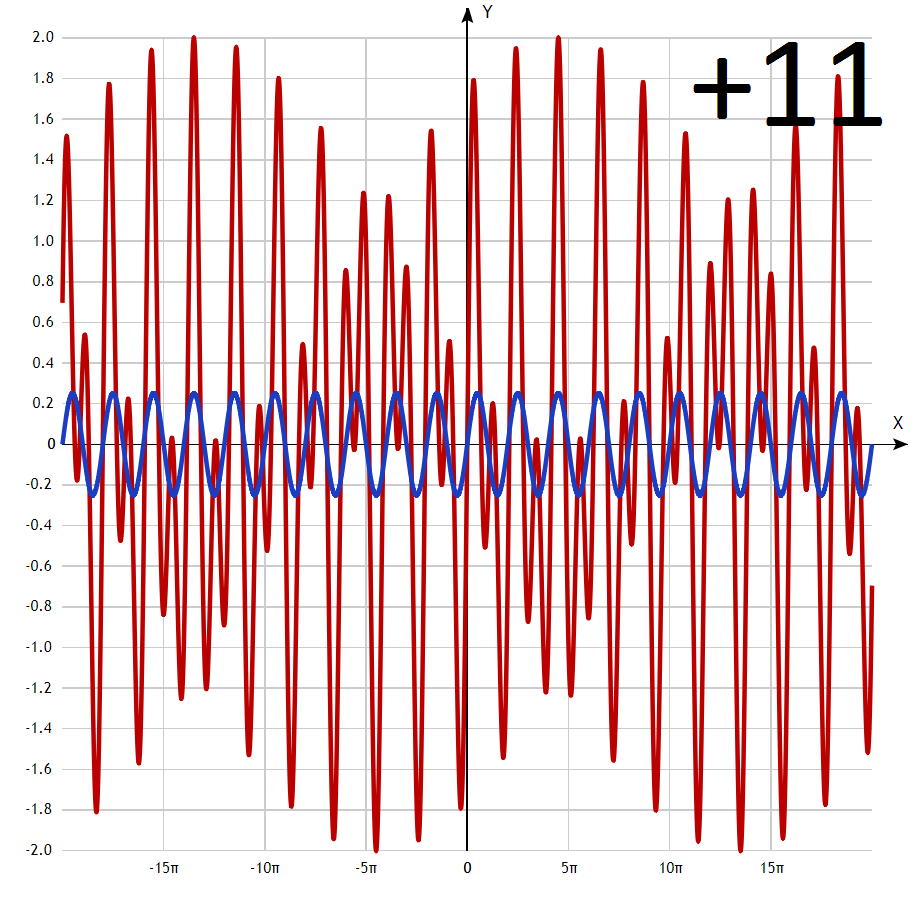
\includegraphics[width=0.45\textwidth]{fig/intervals/i11} \\
        \hline\hline
    \end{tabular}
\end{table}

Приглядитесь к приведенным графикам и попробуйте самостоятельно сделать выводы о причинах благозвучия консонансов и некоей хаотичности диссонансов. Консонансы, кстати, принято разделять на:
\begin{itemize}
    \item \emph{абсолютные}\index{консонанс!абсолютный}. Это полностью сливающиеся на слух интервалы в 0 полутонов (\emph{прима}\index{интервал!прима}, если помните, кстати, \emph{унисон}\index{унисон} --- гармоническая прима) или кратные 12-ти полутонам. О причинах слияния этих звуков мы поговорили в самом начале, см. раздел \ref{ch:music:tone}. Интервал в 12 полутонов, как уже знаем, называется \emph{октавой}\index{интервал!октава}.
    
    \item \emph{совершенные}\index{консонанс!совершенный}. Расстояние между звуками составляет 5(\myNemph{кварта}\index{интервал!кварта}) или 7(\myNemph{квинта}\index{интервал!квинта}) полутонов. См. таблицу \ref{t:harmony:interval:conso-5-7}. Смело можете понизить или повысить любой из звуков такого интервала на одну или несколько октав (12 полутонов) и совершенный консонанс останется\footnote{Уже заметили, что 5+7=12?}. Эти интервалы не сливаются на слух, но звучат благозвучно. Отличник среди консонансов.
    
    \item \emph{несовершенные}\index{консонанс!несовершенный}. Звуки не сливаются, точно не диссонанс, но и не совершенный консонанс. Короче, консонанс с помарочкой. Когда мы слышим несовершенный консонанс, то хочется, чтобы он побыстрее перешел консонанс совершенный, стал отличником. Разница между звуками составляет 3(\myNemph{малая терция}), 4(\myNemph{большая терция}\index{интервал!терция}), 8(\myNemph{малая секста}) или 9(\myNemph{большая секста}\index{интервал!секста}) полутонов. Точно так же, любой звук такого интервала можно понизить или повысить на октаву и несовершенство останется.
\end{itemize}


\begin{table}[!ht]
    \caption{Несовершенные консонансы в графиках \eqref{eq:harmony:interval:sin}}
    \label{t:harmony:interval:conso-3-4-8-9}
    \centering
    \begin{tabular}{c|c}
        \hline\hline
        3 полутона, $n=3$   & 4 полутона, $n=4$ \\
        малая терция        & большая терция \\
        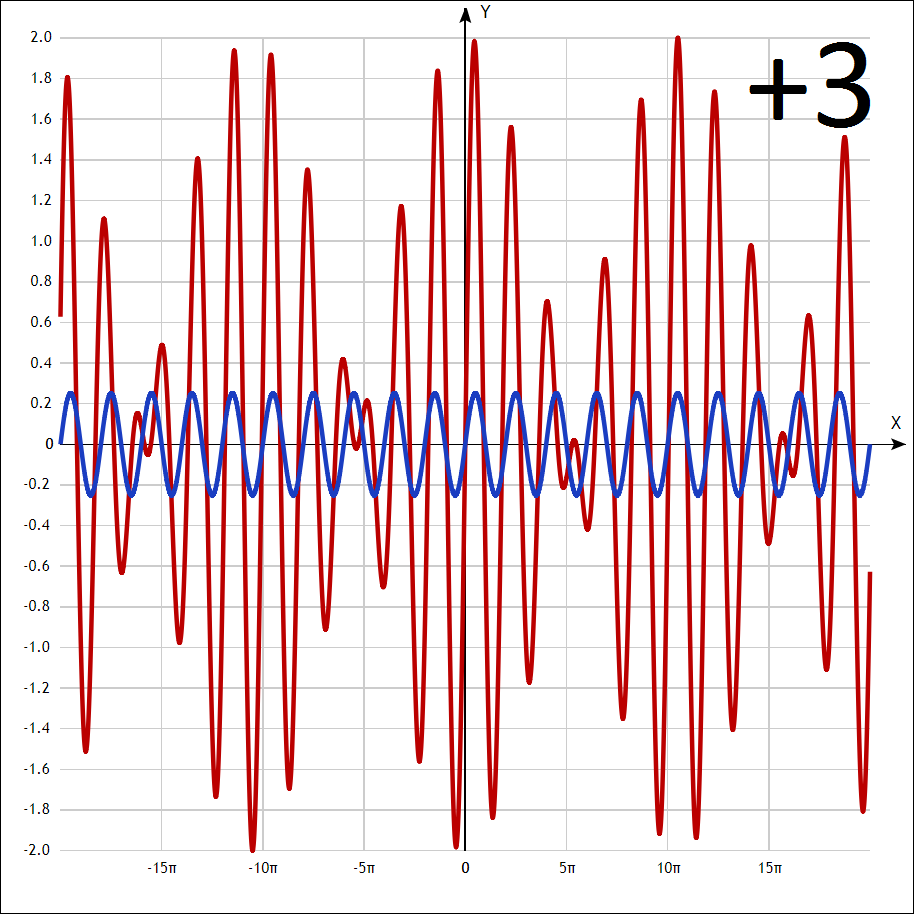
\includegraphics[width=0.45\textwidth]{fig/intervals/i03}
            & 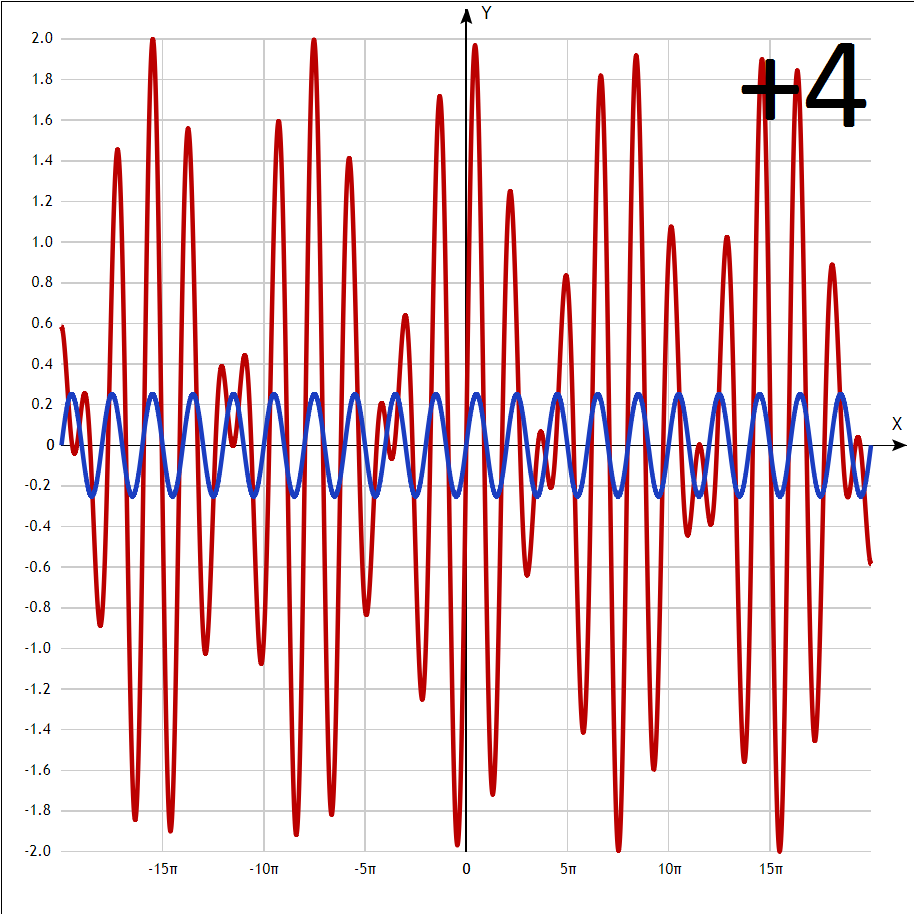
\includegraphics[width=0.45\textwidth]{fig/intervals/i04} \\
        \hline\hline
        8 полутонов, $n=8$  & 9 полутонов, $n=9$ \\
        малая секста        & большая секста \\
        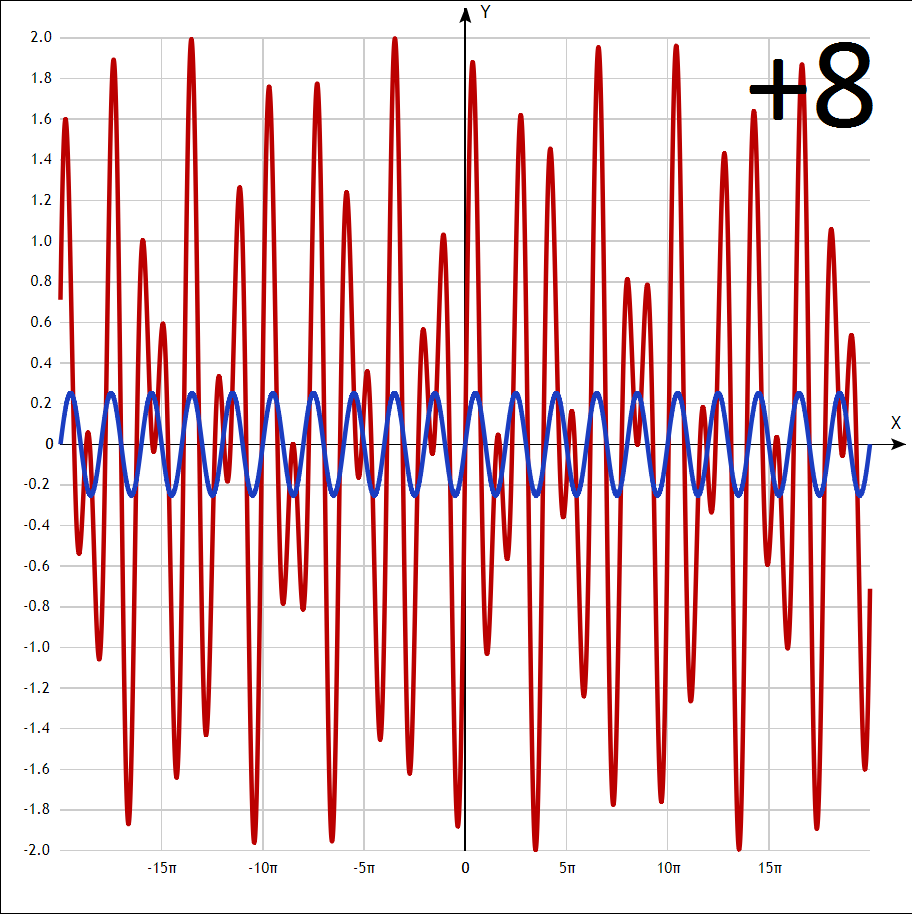
\includegraphics[width=0.45\textwidth]{fig/intervals/i08}
            & 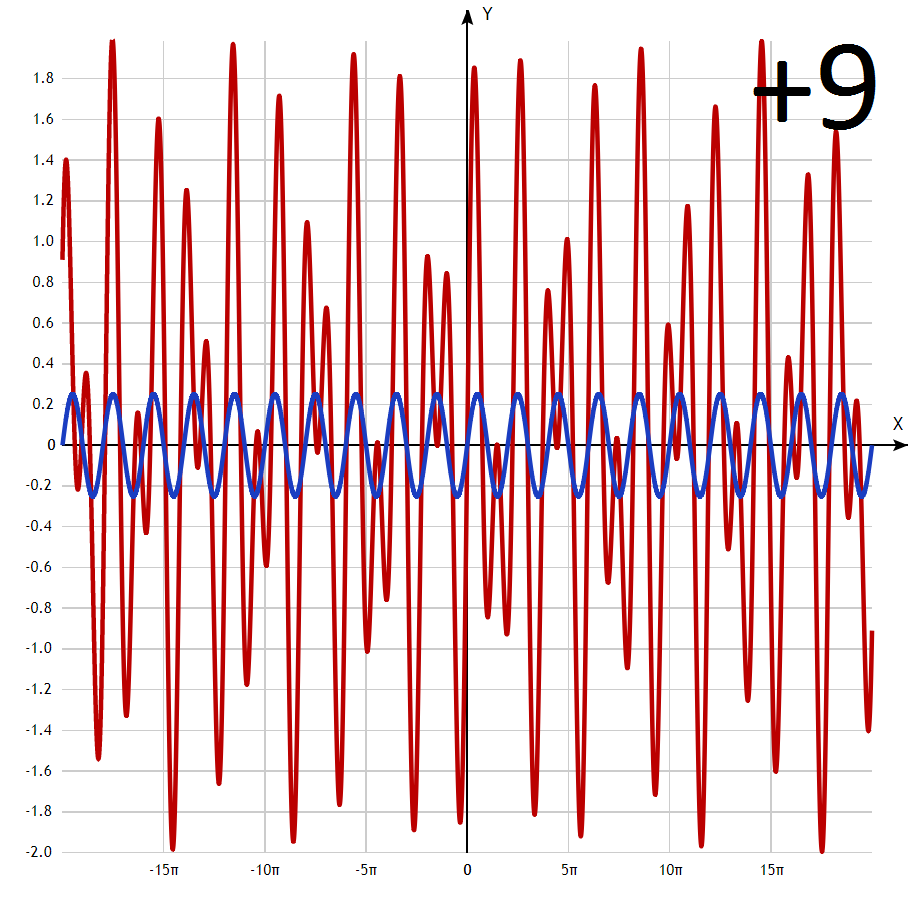
\includegraphics[width=0.45\textwidth]{fig/intervals/i09} \\
        \hline\hline
    \end{tabular}
\end{table}

\begin{table}[!ht]
    \caption{Совершенные консонансы в графиках \eqref{eq:harmony:interval:sin}}
    \label{t:harmony:interval:conso-5-7}
    \centering
    \begin{tabular}{c|c}
        \hline\hline
        5 полутонов, $n=5$  & 7 полутонов, $n=7$ \\
        чистая кварта       & чистая квинта \\
        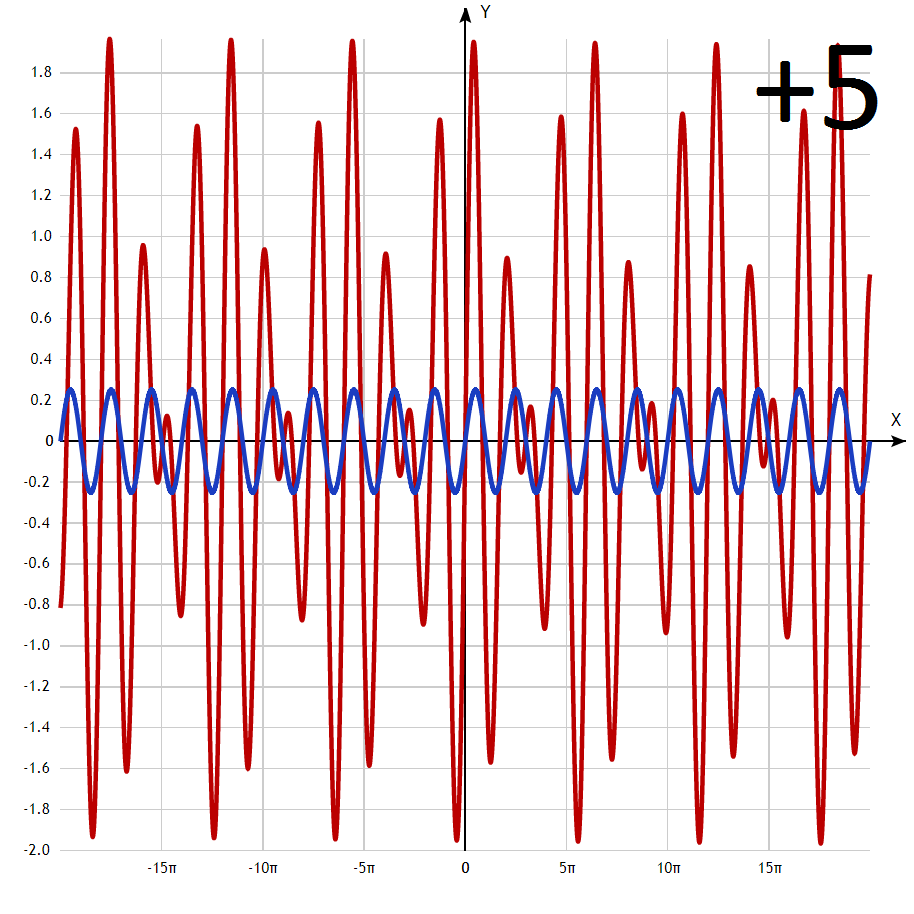
\includegraphics[width=0.45\textwidth]{fig/intervals/i05} 
            & 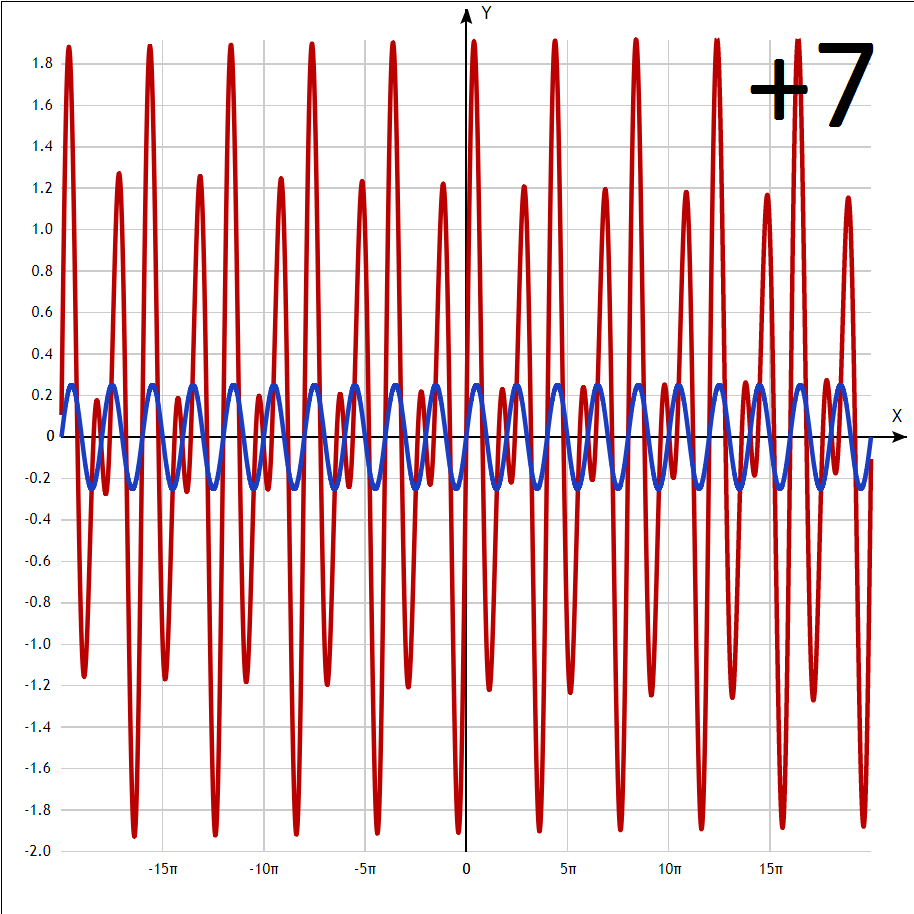
\includegraphics[width=0.45\textwidth]{fig/intervals/i07} \\
        \hline\hline
    \end{tabular}
\end{table}

\begin{table}[!ht]
    \caption{Диссонанс в графике функции \eqref{eq:harmony:interval:sin}}
    \label{t:harmony:interval:disso-6}
    \centering
    \begin{tabular}{c}
        \hline\hline
        6 полутонов, $n=6$ \\
        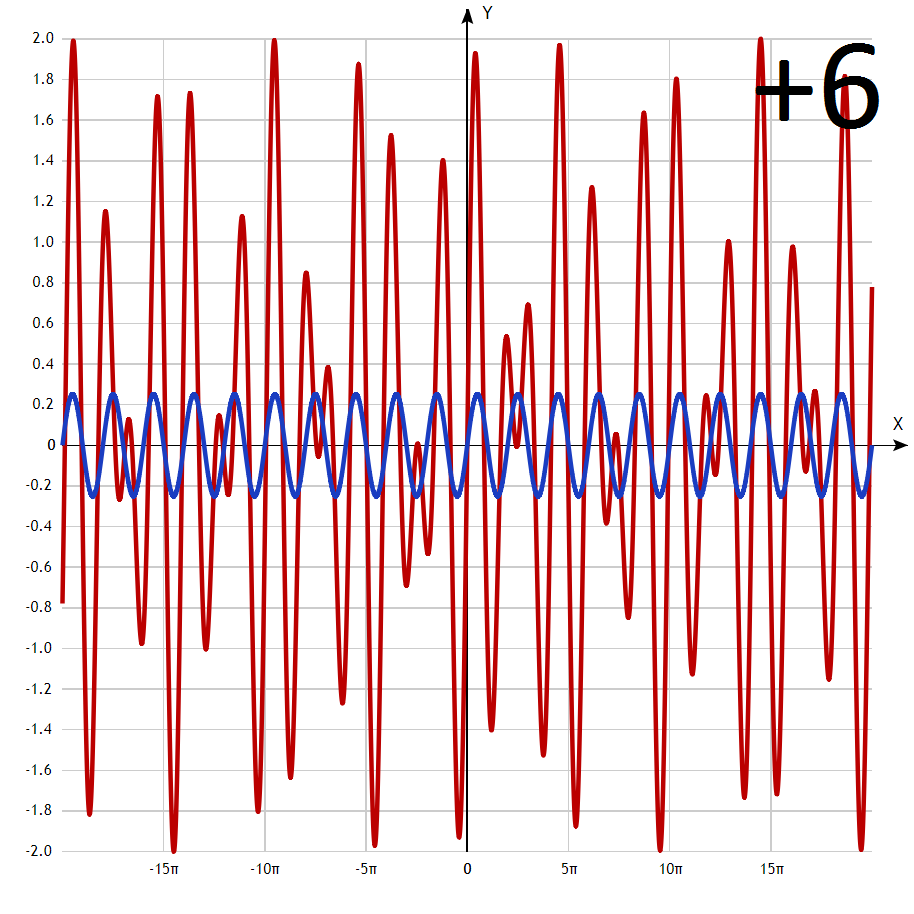
\includegraphics[width=0.45\textwidth]{fig/intervals/i06} \\
        увеличенная кварта,\\
        она же --- уменьшенная квинта,\\
        он же --- тритон\\
        \hline\hline
    \end{tabular}
\end{table}

Звуки октавы удобно зациклить и изобразить на окружности. На рисунке \ref{fig:harmony:interval:oct-round} изображены ноты и отмечены консонансы и диссонансы от ДО (C --- ноты обозначены в латинской нотации). 

\begin{figure}[!ht]
    \centering
    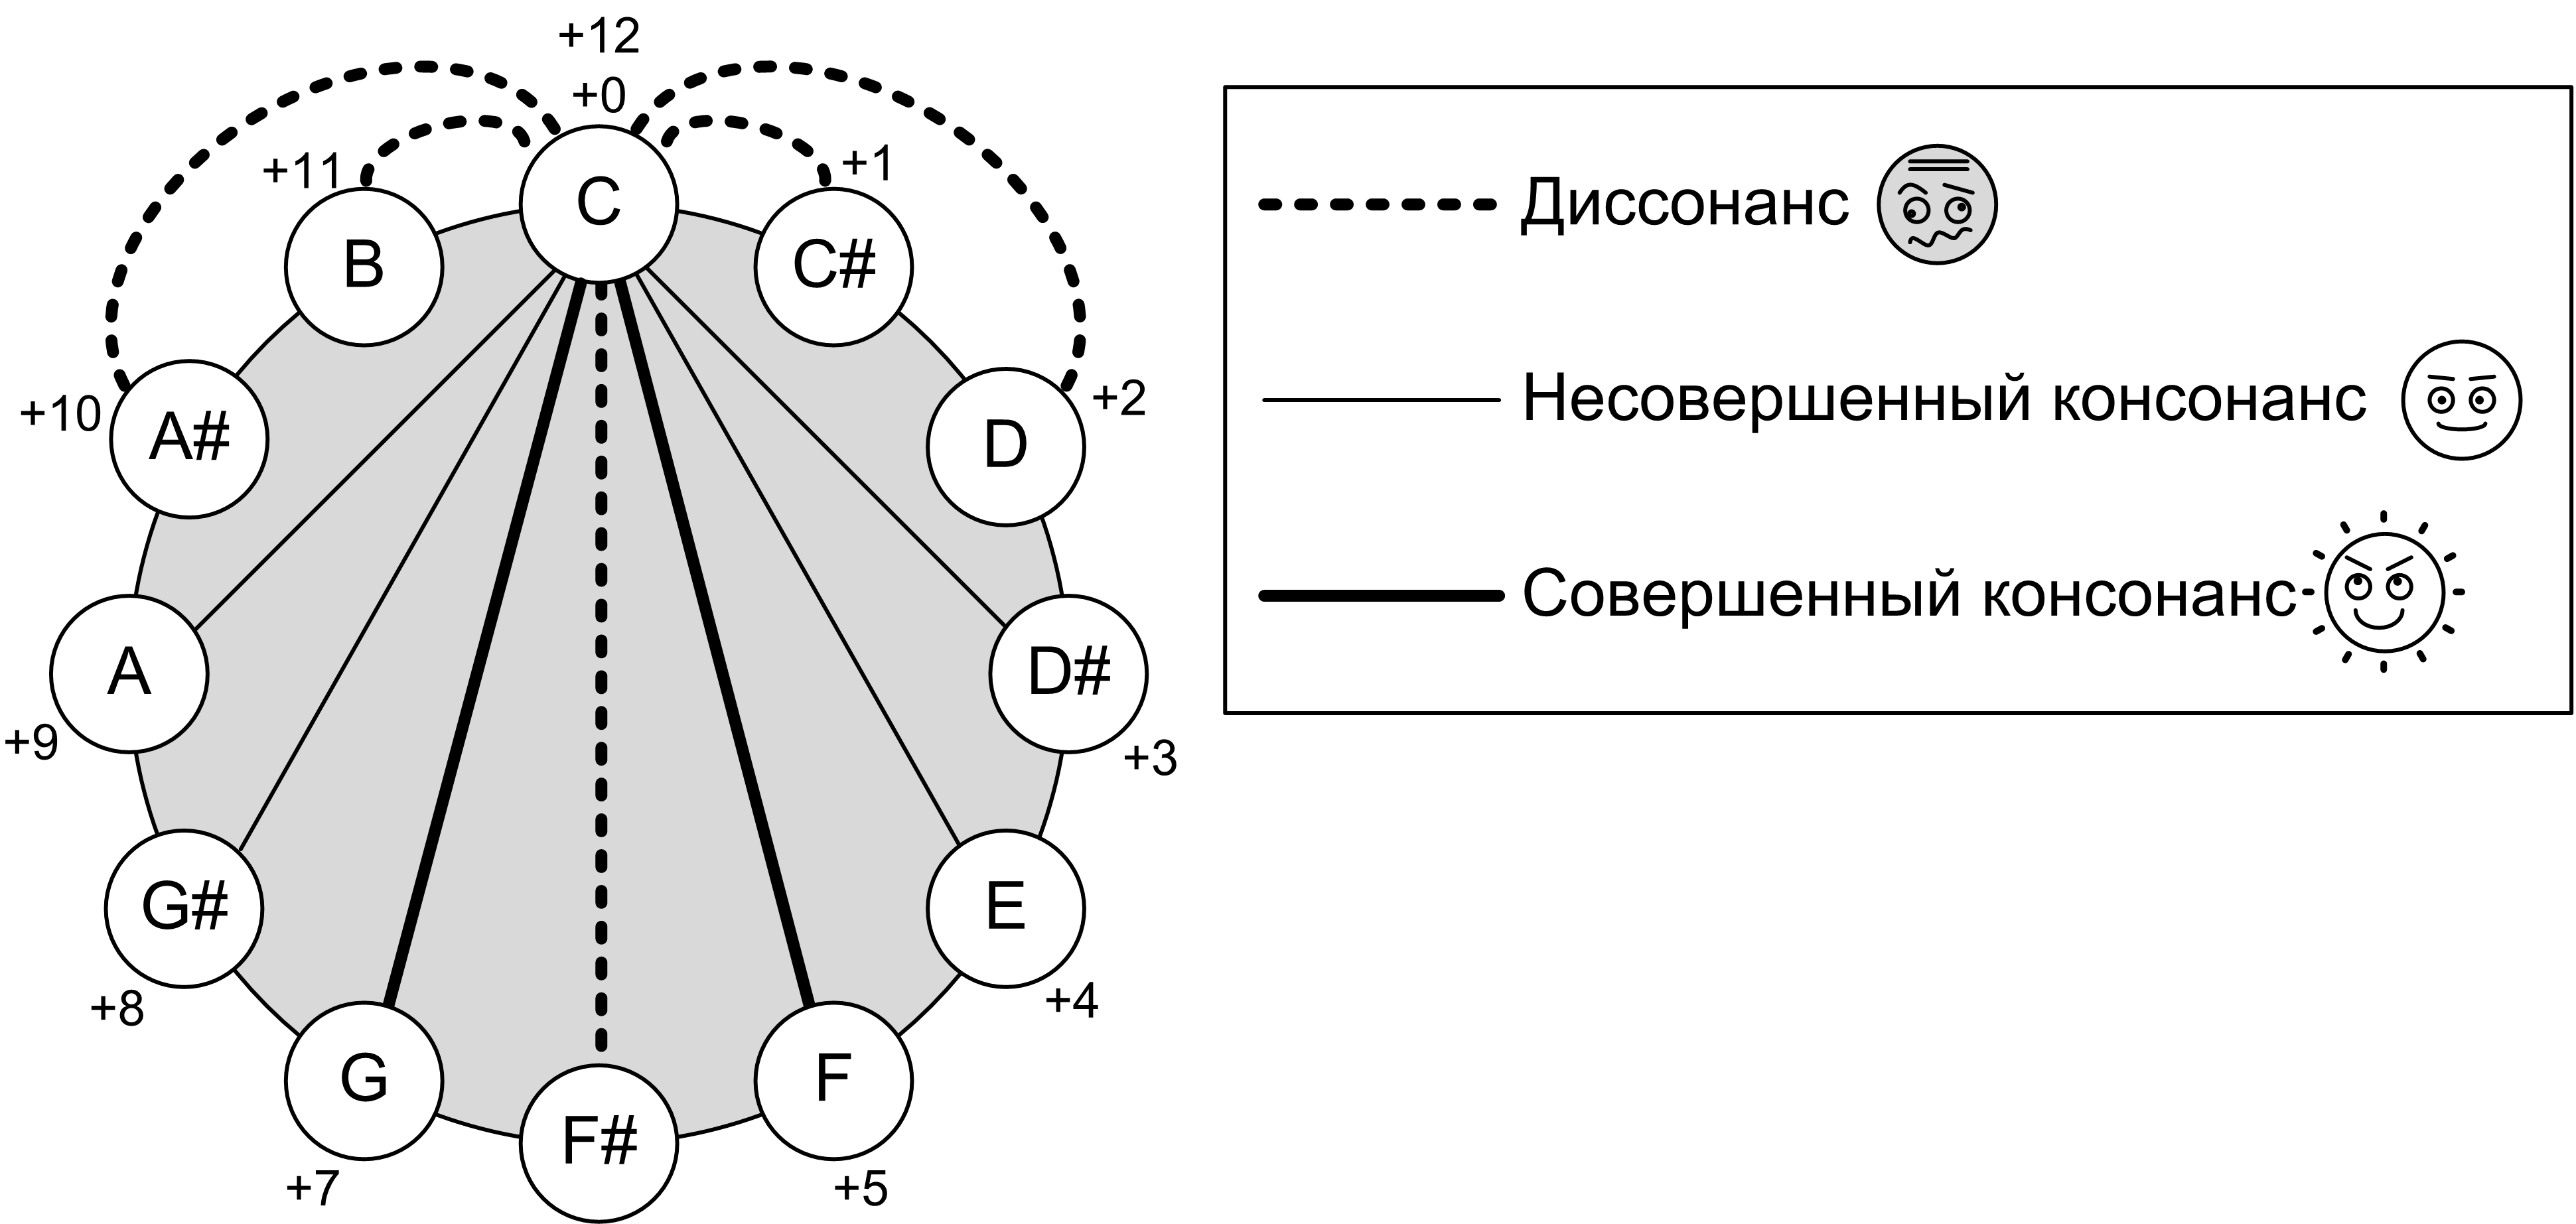
\includegraphics[width=\textwidth]{fig/intervals/octave-round} 
    \caption{Интервалы от ноты ДО}\label{fig:harmony:interval:oct-round}
\end{figure} 

Нужно иметь в виду, что консонансы и диссонансы определяются для любой ноты, поэтому можно не полениться и сделать из картона приборчик, изображенный на рисунке \ref{fig:harmony:interval:octave-kon-dis}: два кружка белый и серый, свободно вращаются на общей оси, проходящей через их центры. Достаточно совместить название ноты на белом кружке со стрелкой на сером и вы узнаете, в каких отношениях указанная нота находится со всеми остальными.

\begin{figure}[!ht]
    \centering
    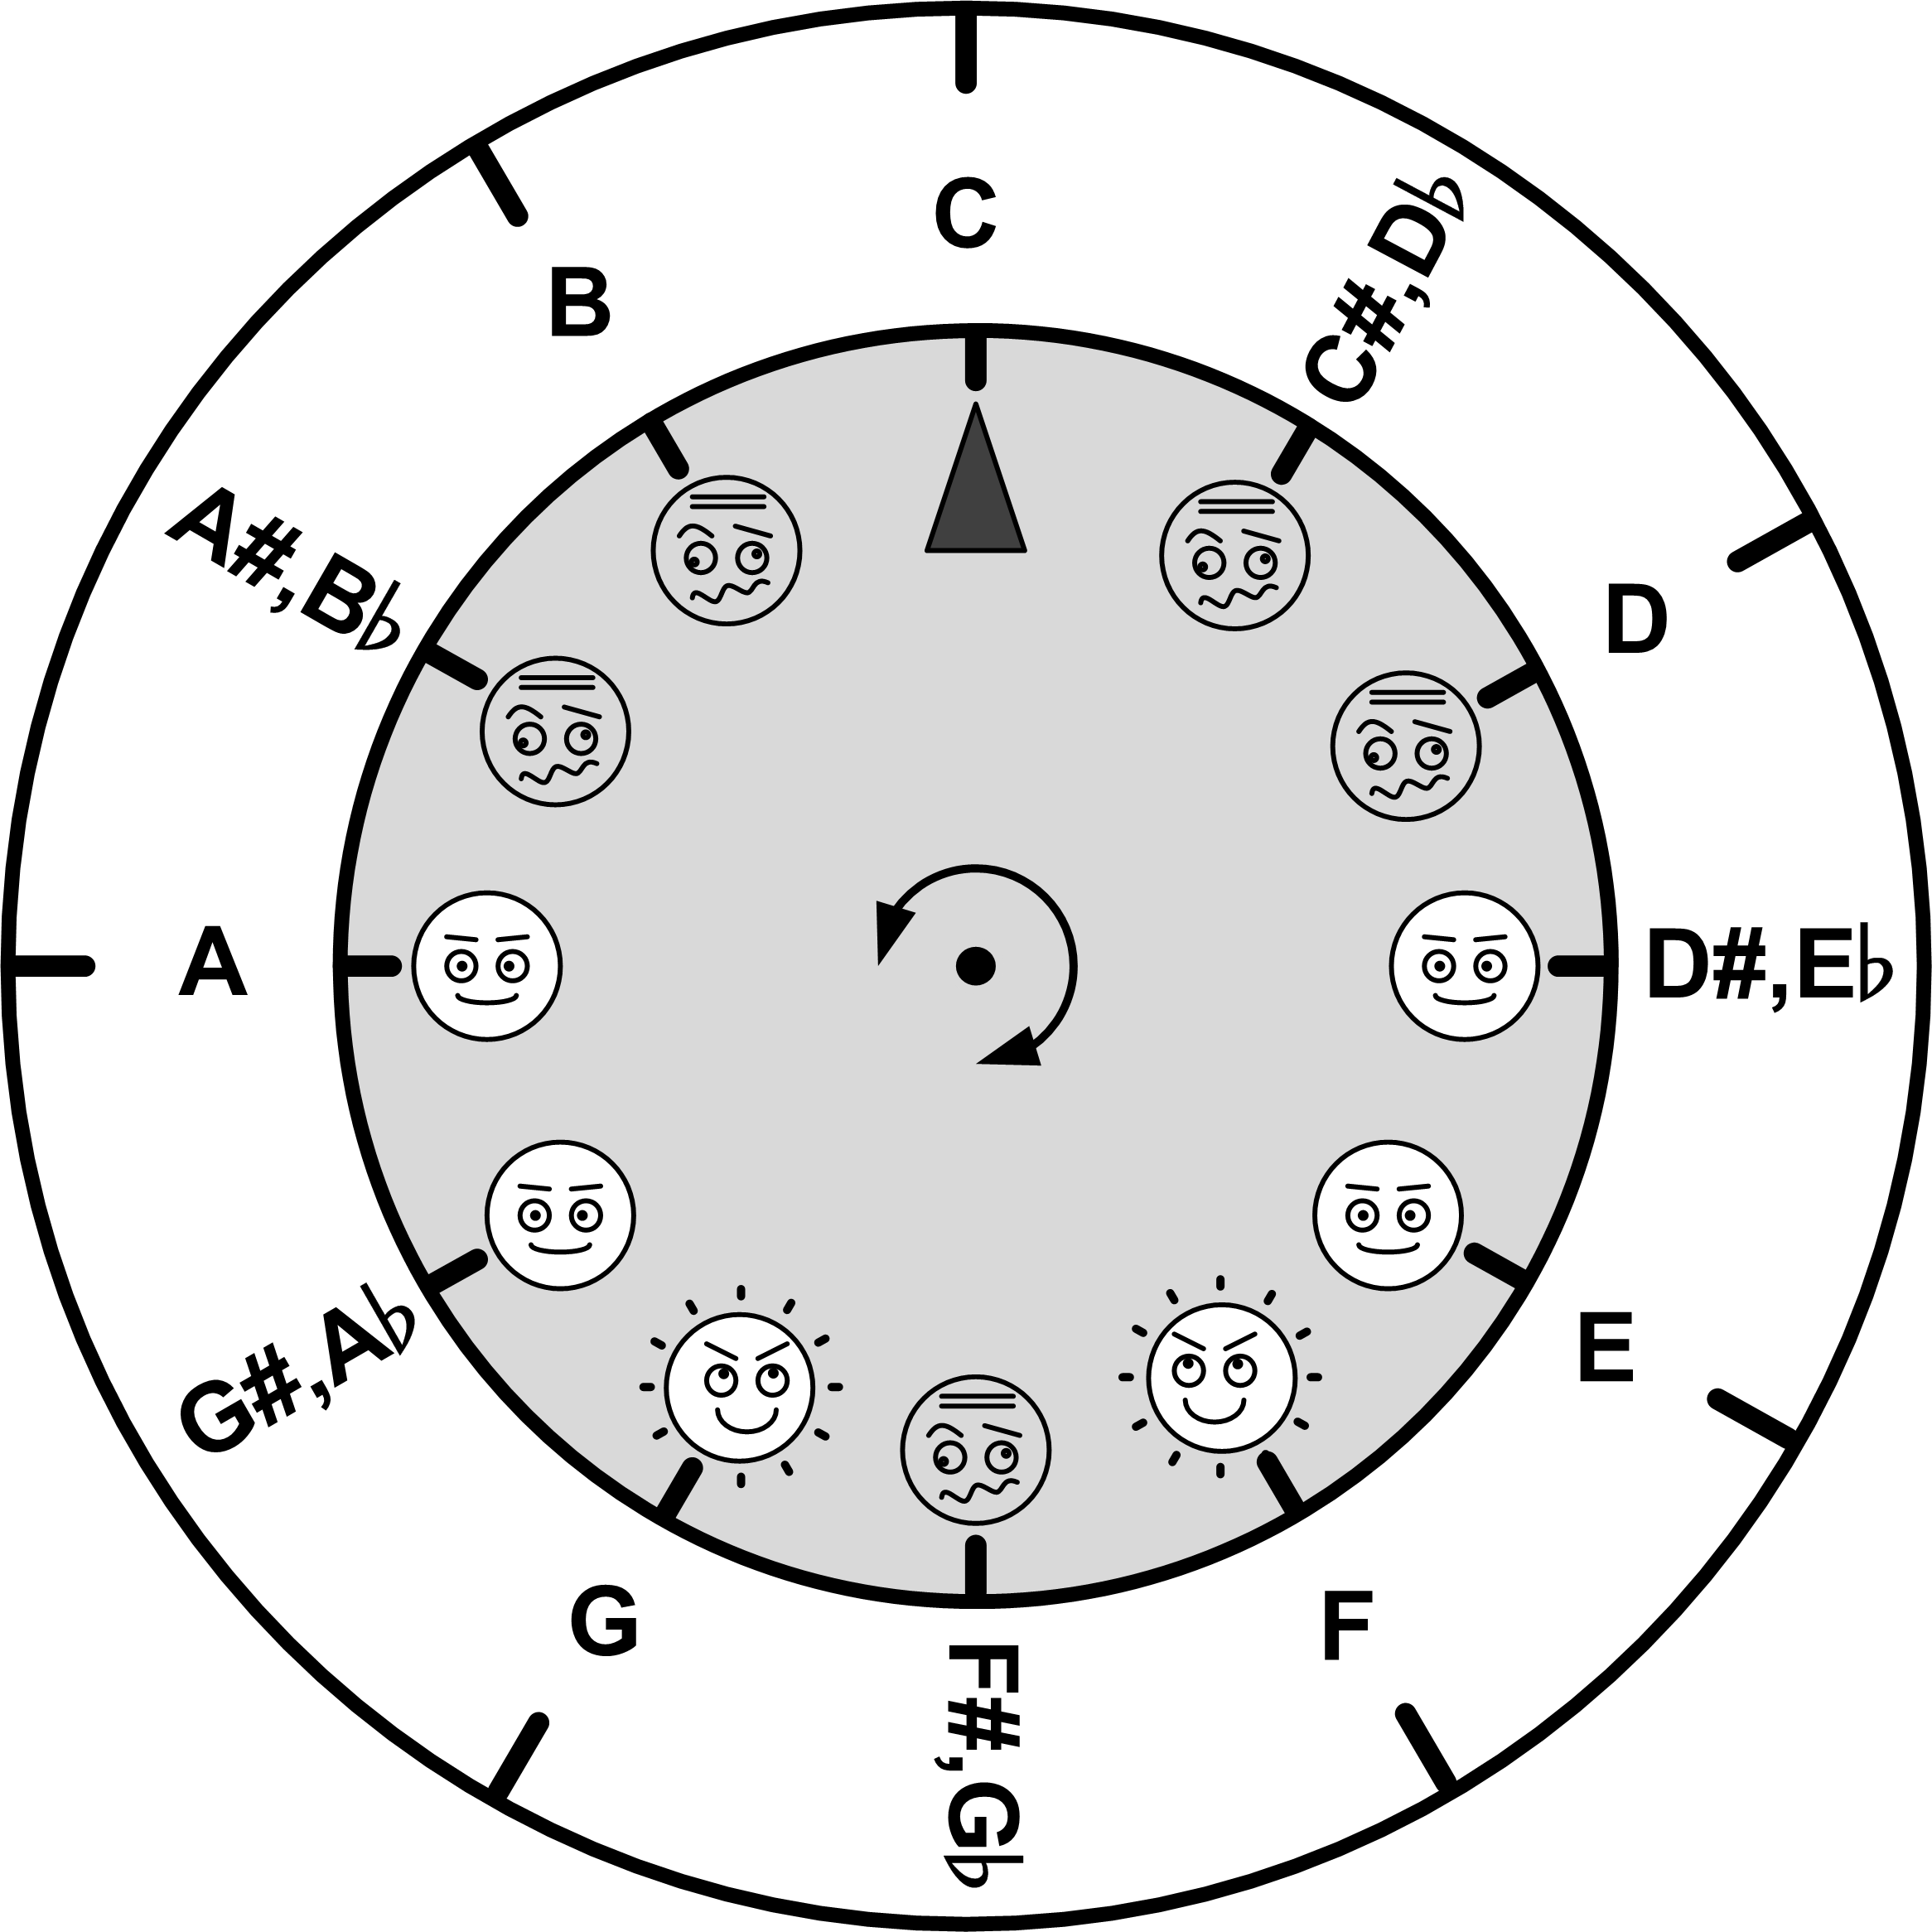
\includegraphics[scale=0.7]{fig/intervals/octave-kon-dis} 
    \caption{Гармонометр}\label{fig:harmony:interval:octave-kon-dis}
\end{figure} 

На практических занятиях с гитарой очень полезной штукой может оказаться <<квинто-квартовый круг мажорных и минорных последовательностей>>, изображенный на рисунке \ref{fig:harmony:kvinto-kvarto:kvinto-kvarto-final} (стр. \pageref{fig:harmony:kvinto-kvarto:kvinto-kvarto-final}). Устройство круга поясняется в разделе \ref{ch:harmony:kvinto-kvarto-round}, но раз уж вы занялись рукоделием, то сделайте и его --- пригодится.

Осталось разобраться, с какой стати интервалы называются так странно? Нет никакой видимой связи между названиями интервала и количеством полутонов, его составляющих! Справочник\footnote{Для тех, кому зубрёжка покажется проще понимания} по интервалам см. в таблице \ref{t:harmony:interval:names}. Собственно, ответ прост: по историческим причинам название интервала отражало не количество полутонов, а номер ступени мажорного музыкального лада (о ладах см. раздел \ref{ch:harmony:lad}). Так как каждая ступенька мажорного лада состояла из одного или двух полутонов, то определить количество полутонов по названию интервала без достаточного опыта затруднительно, если не представить в уме рисунок \ref{fig:harmony:interval:names}.

\begin{table}[!ht]
    \caption{Интервалы\index{интервал}}
    \label{t:harmony:interval:names}
    \centering
    \begin{tabular}{l|l|l|c|l}
        \hline\hline
        Название интервала & Перевод            &               & Количество  & Кратко  \\
                           & на Русский         &               & полутонов   &         \\
        \hline\hline
        Прима(prima)       & Первая (ступень)   & Чистая        & 0                 & ч.1 \\
        Секунда(secunda)   & Вторая             & Малая         & 1                 & м.2 \\
                           &                    & Большая       & 2                 & б.2 \\
        Терция(tertia)     & Третья             & Малая         & 3                 & м.3 \\
                           &                    & Большая       & 4                 & б.3 \\
        Кварта(quarta)     & Четвертая          & Чистая        & 5                 & ч.4 \\
                           &                    & Увеличенная   & 6                 & ув.4\\
        Квинта(quinta)     & Пятая              & Уменьшенная   & 6                 & ум.5\\
                           &                    & Чистая        & 7                 & ч.5 \\
        Секста(sexta)      & Шестая             & Малая         & 8                 & м.6 \\
                           &                    & Большая       & 9                 & б.6 \\
        Септима(septima)   & Седьмая            & Малая         & 10                & м.7 \\
                           &                    & Большая       & 11                & б.7 \\
        Октава(octava)     & Восьмая            & Чистая        & 12                & ч.8 \\
        \hline\hline
        Нона(nona)         & Девятая            & Малая         & 13                & м.9  \\
                           &                    & Большая       & 14                & б.9  \\
        Децима(decima)     & Десятая            & Малая         & 15                & м.10 \\
                           &                    & Большая       & 16                & б.10 \\
        Ундецима           & Одиннадцатая       & Чистая        & 17                & ч.11 \\
                           &                    & Увеличенная   & 18                & ув.11\\
        Дуодецима          & Двенадцатая        & Уменьшенная   & 18                & ум.12\\
                           &                    & Чистая        & 19                & ч.12 \\
        Терцдецима         & Тринадцатая        & Малая         & 20                & м.13 \\
                           &                    & Большая       & 21                & б.13 \\
        Квартдецима        & Четырнадцатая      & Малая         & 22                & м.14 \\
                           &                    & Большая       & 23                & б.14 \\
        Квинтдецима        & Пятнадцатая        & Чистая        & 24                & ч.15 \\
        \hline\hline
    \end{tabular}
\end{table}

\begin{figure}[!ht]
    \centering
    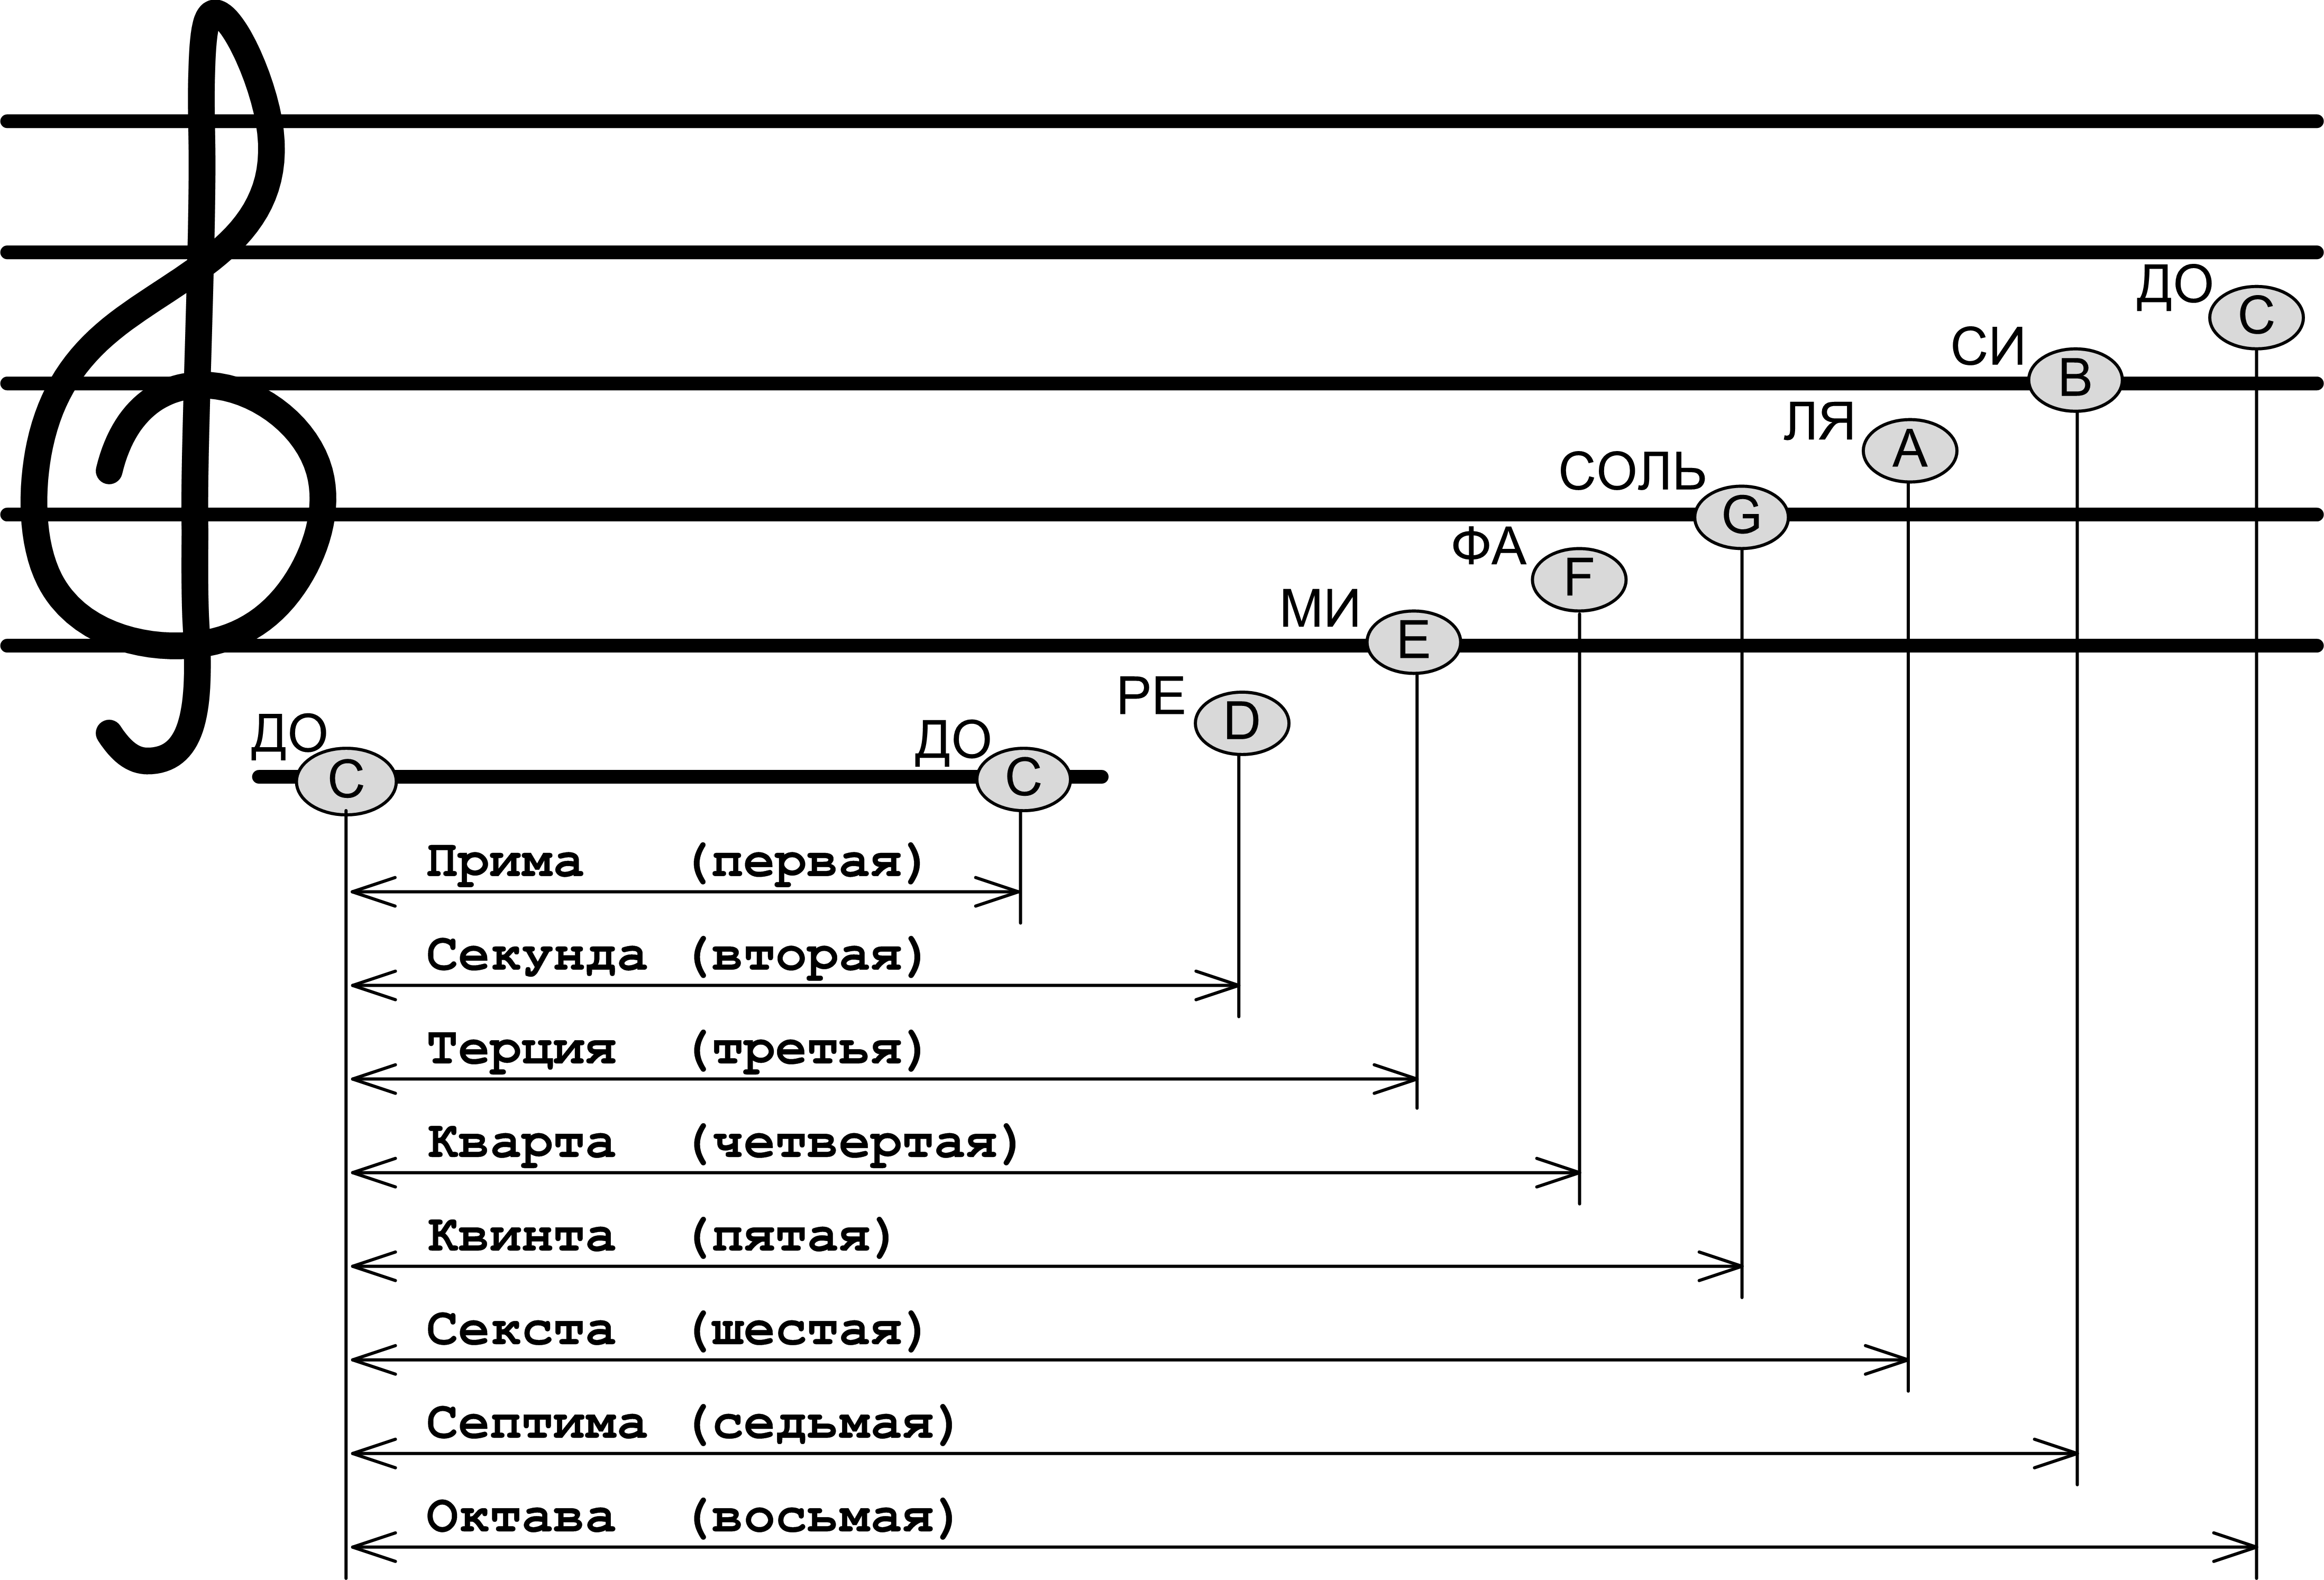
\includegraphics[width=.9\textwidth]{fig/intervals/interval-names} 
    \caption{Исторически имена интервалов\index{интервал} --- это имена ступеней мажорного лада}\label{fig:harmony:interval:names}
\end{figure} 

Действительно, названия интервалов --- это всего-лишь порядковый номер (на латинском) ступени мажорного лада. Тогда всё становится относительно просто. Например, терция, это расстояние от ноты ДО (первая-прима ступень мажорного лада) до ноты МИ (третья-терция ступень). Считаем ДО-РЕ --- 2 полутона, РЕ-МИ --- 2-а полутона. Получилось 4-е полутона. Только вот вспоминается, что терция бывает <<большая>> и <<малая>>. Считая расстяние от ноты ДО до соответствующей ступени, мы всегда будем получать значение для <<большого>> и <<чистого>> интервалов. Для <<малого>> или <<уменьшенного>> интервалов нужно уменьшить количество полутонов чистого интервала на 1, а для <<увеличенного>> --- увеличить на 1. Значит: большая терция --- 4 полутона, малая --- 3.

Закрепим. Например, квинта: расстояние ДО-СОЛЬ --- 7 полутонов. Уменьшенная квинта --- 6 полутонов, чистая --- 7, увеличенная --- не прижилась.

\section{Лады? Лады}
\label{ch:harmony:lad}

\begin{Definition}[Лад]
    \emph{Лад}\footnote{На английском \emph{лад} --- \emph{mode}. Режим работы, способ, вид, метод} --- это интервальный шаблон, позволяющий из 12-и последовательных музыкальных звуков октавы выбрать \emph{условно} <<правильные>>. 
\end{Definition}

Если это определение показалось вам тяжеловатым, почитайте учебники или Википедию. От некоторых определений веет такой суровой философией, что хочется курить в глубокий затяг. 

Задача лада: из 12 музыкальных звуков, составляющих октаву, выбрать лишь несколько таких, которые можно играть в любом порядке и все равно будет МУЗЫКА! Задача не из тривиальных и кажется весьма субъективной, ведь всегда найдется кто-то, кто скажет: <<А мне не нравится!>>. 

Однако эта задача была решена\footnote{Не исключено, что кем-то она решается и в данный момент} предками неоднократно, и в культурном наследнии мы имеем немало ладов, самыми известными из которых являются \emph{мажорный} и \emph{минорный}.

Мажорный и минорный лады --- лады \emph{семиступенные}. То есть такой лад выбирает из 12 звуков октавы только 7.

\paragraph{Мажорный лад.} Начнем с мажорного лада, интервальная структура которого приведена на рисунке \ref{fig:harmony:lad:mode:maj}. Тёмными кружками обозначены <<выбранные>> ладом звуки --- \emph{ступени} лада. Например, вторая ступень мажорного лада находится на расстоянии 2-х полутонов от первой. Интервалы (в полутонах) между ступенями \emph{мажорного} лада расположены так:

\[
    \texttt{2-2-1-2-2-2-1}
\]

Всем с детства знакомое ДО, РЕ, МИ, ФА, СОЛЬ, ЛЯ, СИ есть не что иное, как 7 идеальных ноток, отобранных мажорным ладом, начиная от ноты ДО. Проверьте: (ДО-РЕ)=2 полутона, (РЕ-МИ)=2, (МИ-ФА)=1, (ФА-СОЛЬ)=2 и т.д. 

Интересно то, что уникальные имена получили только 7 нот, а остальные 5 нот октавы имеют производные имена (с суффиксом <<бемоль>> или <<диез>>) --- есть следствие использования ладов.

\begin{figure}[!ht]
    \centering
    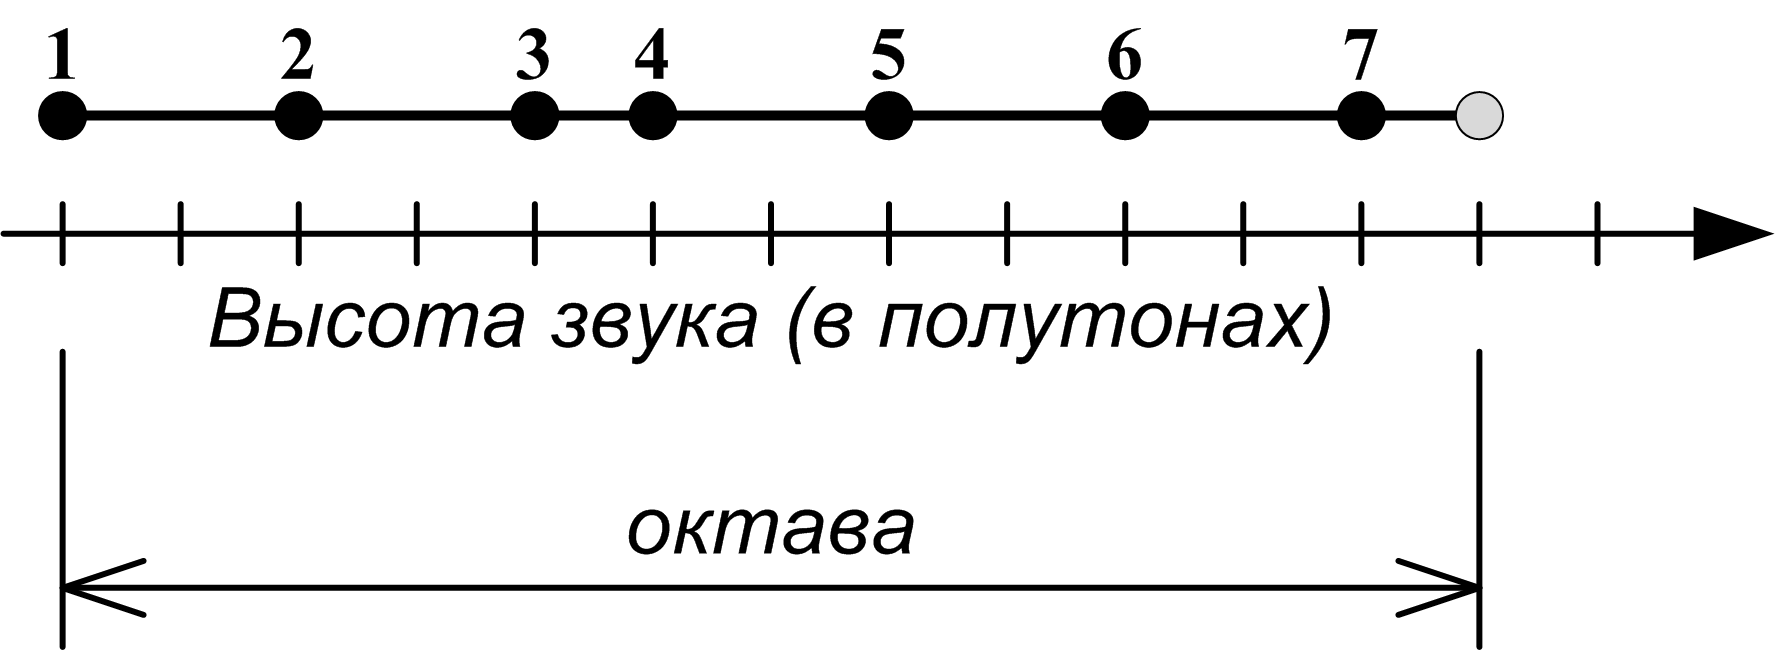
\includegraphics{fig/intervals/mode-maj} 
    \caption{Интервальная структура мажорного лада}\label{fig:harmony:lad:mode:maj}
\end{figure} 

Таким образом, шаблон лада может накладываться на любую ноту, любой музыкальный звук. Сплошная теория относительности!

Когда первая ступень лада накладывается на определенную ноту, то набор нот, попавших на ступени лада, образует \emph{тональность}\footnote{На английском \emph{тональность} --- tonality}. Допустим, мы совместили первую ступень мажорного лада с нотой ДО, тогда мы получим тональность <<ДО-мажор>>: 
\[
    \text{ДО}\xrightarrow{2}
    \text{РЕ}\xrightarrow{2}
    \text{МИ}\xrightarrow{1}
    \text{ФА}\xrightarrow{2}
    \text{СОЛЬ}\xrightarrow{2}
    \text{ЛЯ}\xrightarrow{2}
    \text{СИ}\xrightarrow{1}
\]

Базовая нота, т.е. нота, на которую наложили перую ступень лада, называется \emph{тоникой}\footnote{Ступени мажорного и минорного ладов так часто используются в теории музыки, что получили собственные названия. Нам, чтобы разобраться, достаточно запомнить, что нота, попавшая в первую ступень называется \emph{тоника}. А для общего развития: 5-я ступень --- доминанта, 4-я --- субдоминанта, 3-я --- медианта. Повторюсь: это названия ступеней как мажорного, так и минорного ладов}.

Название тональности складывается из названия ноты, попавшей на первую ступень (\emph{тоники}) и названия лада. Обычно мелодия составляется только из семи нот, входящих в тональность. Так и говорят, например, мелодия в тональности <<ЛЯ-минор>>.

\begin{Example}[Тональность <<РЕ-мажор>>]
    \label{ex:harmony:lad:d:maj}
    
    Чтобы получить ноты в тональности РЕ-мажор, нам нужно совместить ноту РЕ и первую ступень мажорного лада. Отступаем два полутона, и на вторую ступень попадет нота МИ. На третью --- ФА-диез.
    
    Целиком:
    \[
        \text{РЕ}\xrightarrow{2} 
        \text{МИ}\xrightarrow{2} 
        \text{ФА-диез}\xrightarrow{1} 
        \text{СОЛЬ}\xrightarrow{2} 
        \text{ЛЯ}\xrightarrow{2} 
        \text{СИ}\xrightarrow{2} 
        \text{ДО-диез}\xrightarrow{1}
    \]
    
    В эту тональность попали нотки, имеющие производные названия: ФА-диез, ДО-диез.
\end{Example}

Задача определить ноты, входящие в ту или иную тональность, а также количество диезов и бемолей, является любимой пыткой среди музыкальных инквизиторов. Сдвинуть шаблончик --- дело плёвое. А вот ноты после этого назвать --- уже подвиг! Совершенно искусственная проблема, растущая только от принятого способа обозначать ноты.

Например, для певца, поющего по нотам\footnote{Да, есть люди которые могут делать такие штуки со своим голосом: тянуть гласные с нужной частотой основного тона} чтобы перейти из тональности <<ДО-мажор>> в <<РЕ-мажор>> достаточно каждую исходную нотку спеть двумя полутонами выше (сдвинуть шаблон) и не думать о том, какая нота получается в итоге (закодировать название ноты).

Характерная ситуация в музыке: с практической точки зрения все оказывается проще, чем с теоретической!

Чтобы сыграть \emph{гамму}\footnote{Слово \emph{гамма} в русском очень похоже на \emph{Game} (игра) в английском. И вроде бы логично: гамма --- это то, что \emph{играется}! Но \emph{гамма} на английском --- \emph{scale}. Шкала, звукоряд} в заданной тональности нужно:
\begin{itemize}
    \item начать с ноты первой ступени;
    \item продолжить играть ноты тональности в порядке возрастания (или убывания) высоты;
    \item сыграв таким образом одну или несколько октав, закончить на ноте первой ступени (естественно уже в другой октаве); 
    \item (необязательно) проиграть только что сыгранную последовательность в обратном порядке.
\end{itemize}

Например, гамма в тональности <<ДО-мажор>> или просто <<гамма ДО-мажор>> это известное: 
\begin{center}
    ДО, РЕ, МИ, ФА, СОЛЬ, ЛЯ, СИ, ДО, СИ, ЛЯ, СОЛЬ, ФА, МИ, РЕ, ДО.
\end{center}


\paragraph{Минорный лад.} Интервальная структура \emph{минорного} лада приведена на рисунке \ref{fig:harmony:lad:mode:min}. Интервалы (в полутонах) между ступенями \emph{минорного} лада расположены так:
\[
    \texttt{2-1-2-2-1-2-2}
\]

\begin{figure}[!ht]
    \centering
    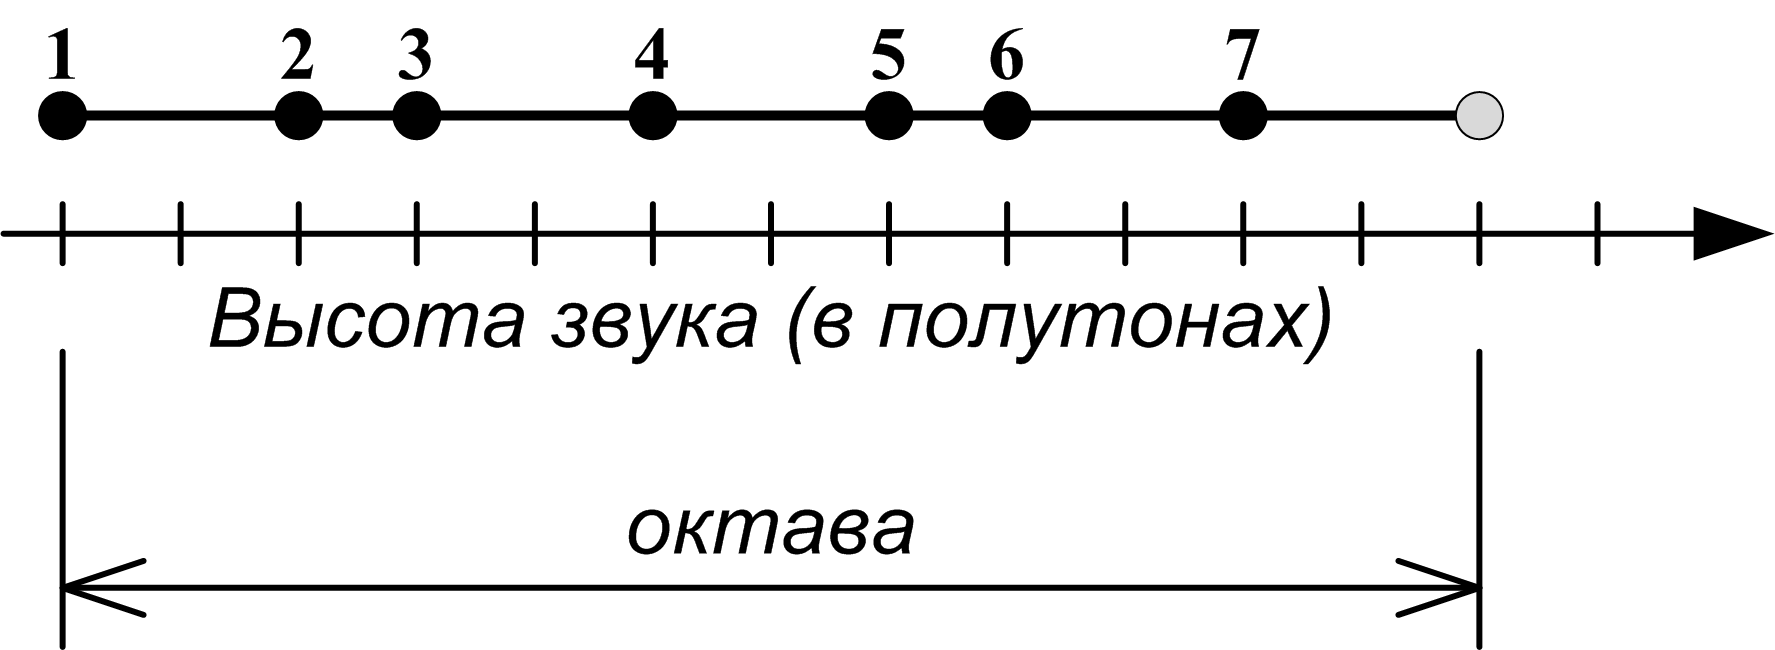
\includegraphics{fig/intervals/mode-min} 
    \caption{Интервальная структура минорного лада}\label{fig:harmony:lad:mode:min}
\end{figure} 

Заметьте, что если замкнуть минорную интервальную структуру в кольцо и немного повращать (а это можно сделать, так как в следующей октаве все повторится), то получится мажорный лад. Совместите первую ступень мажорного лада и третью минорного и убедитесь, что в принципе структура этих ладов одна и та же. 

Например, давайте положим в первую ступень минора ноту ЛЯ. Получим тональность, состоящую из нот:
\begin{center}
    ЛЯ, СИ, ДО, РЕ, МИ, ФА, СОЛЬ.
\end{center}

Названия нот в тональности <<ЛЯ-минор>> те же, что и в <<ДО-мажор>> (как видно, нет ни одной нотки с бемолем или диезом). Поэтому тональности <<ДО-мажор>> и <<ЛЯ-минор>> называются \emph{параллельными}. Как нетрудно догадаться, параллельных тональностей столько же, сколько нот в октаве: 12. А вот \emph{гамму} <<ЛЯ-минор>>:
\begin{center}
    ЛЯ, СИ, ДО, РЕ, МИ, ФА, СОЛЬ, ЛЯ, СОЛЬ, ФА, МИ, РЕ, ДО, СИ, ЛЯ
\end{center}
с гаммой <<ДО-мажор>> точно на слух не спутаешь!

\paragraph{Современные 7-ступенные лады.} Эти лады имеют сходную интервальную структуру и называются диатоническими\footnote{Диатонические лады или просто <<диатоника>> --- это система семиступенных ладов, постоенных из пяти интервалов величиной в два полутона, и двух полутоновых интервалов. $5\cdot2 + 2\cdot 1 = 12$ --- октава}. Мажор и минор --- также диатонические лады. На рисунке \ref{fig:harmony:lad:modes} иображена октава, разделенная на 12 полутонов. Лады отличаются друг от друга только тем, откуда начинается первая ступень. Каждый из семи возможных вариантов имеет собственное название. 

Например, первая ступень <<Лидийского>> лада начинается с 4-й отметки на октаве, и, обойдя от 4-й отметки всю окраву, легко получить его интервальную структуру:
\[
    \texttt{2-2-2-1-2-2-1}
\]

\begin{figure}[!ht]
    \centering
    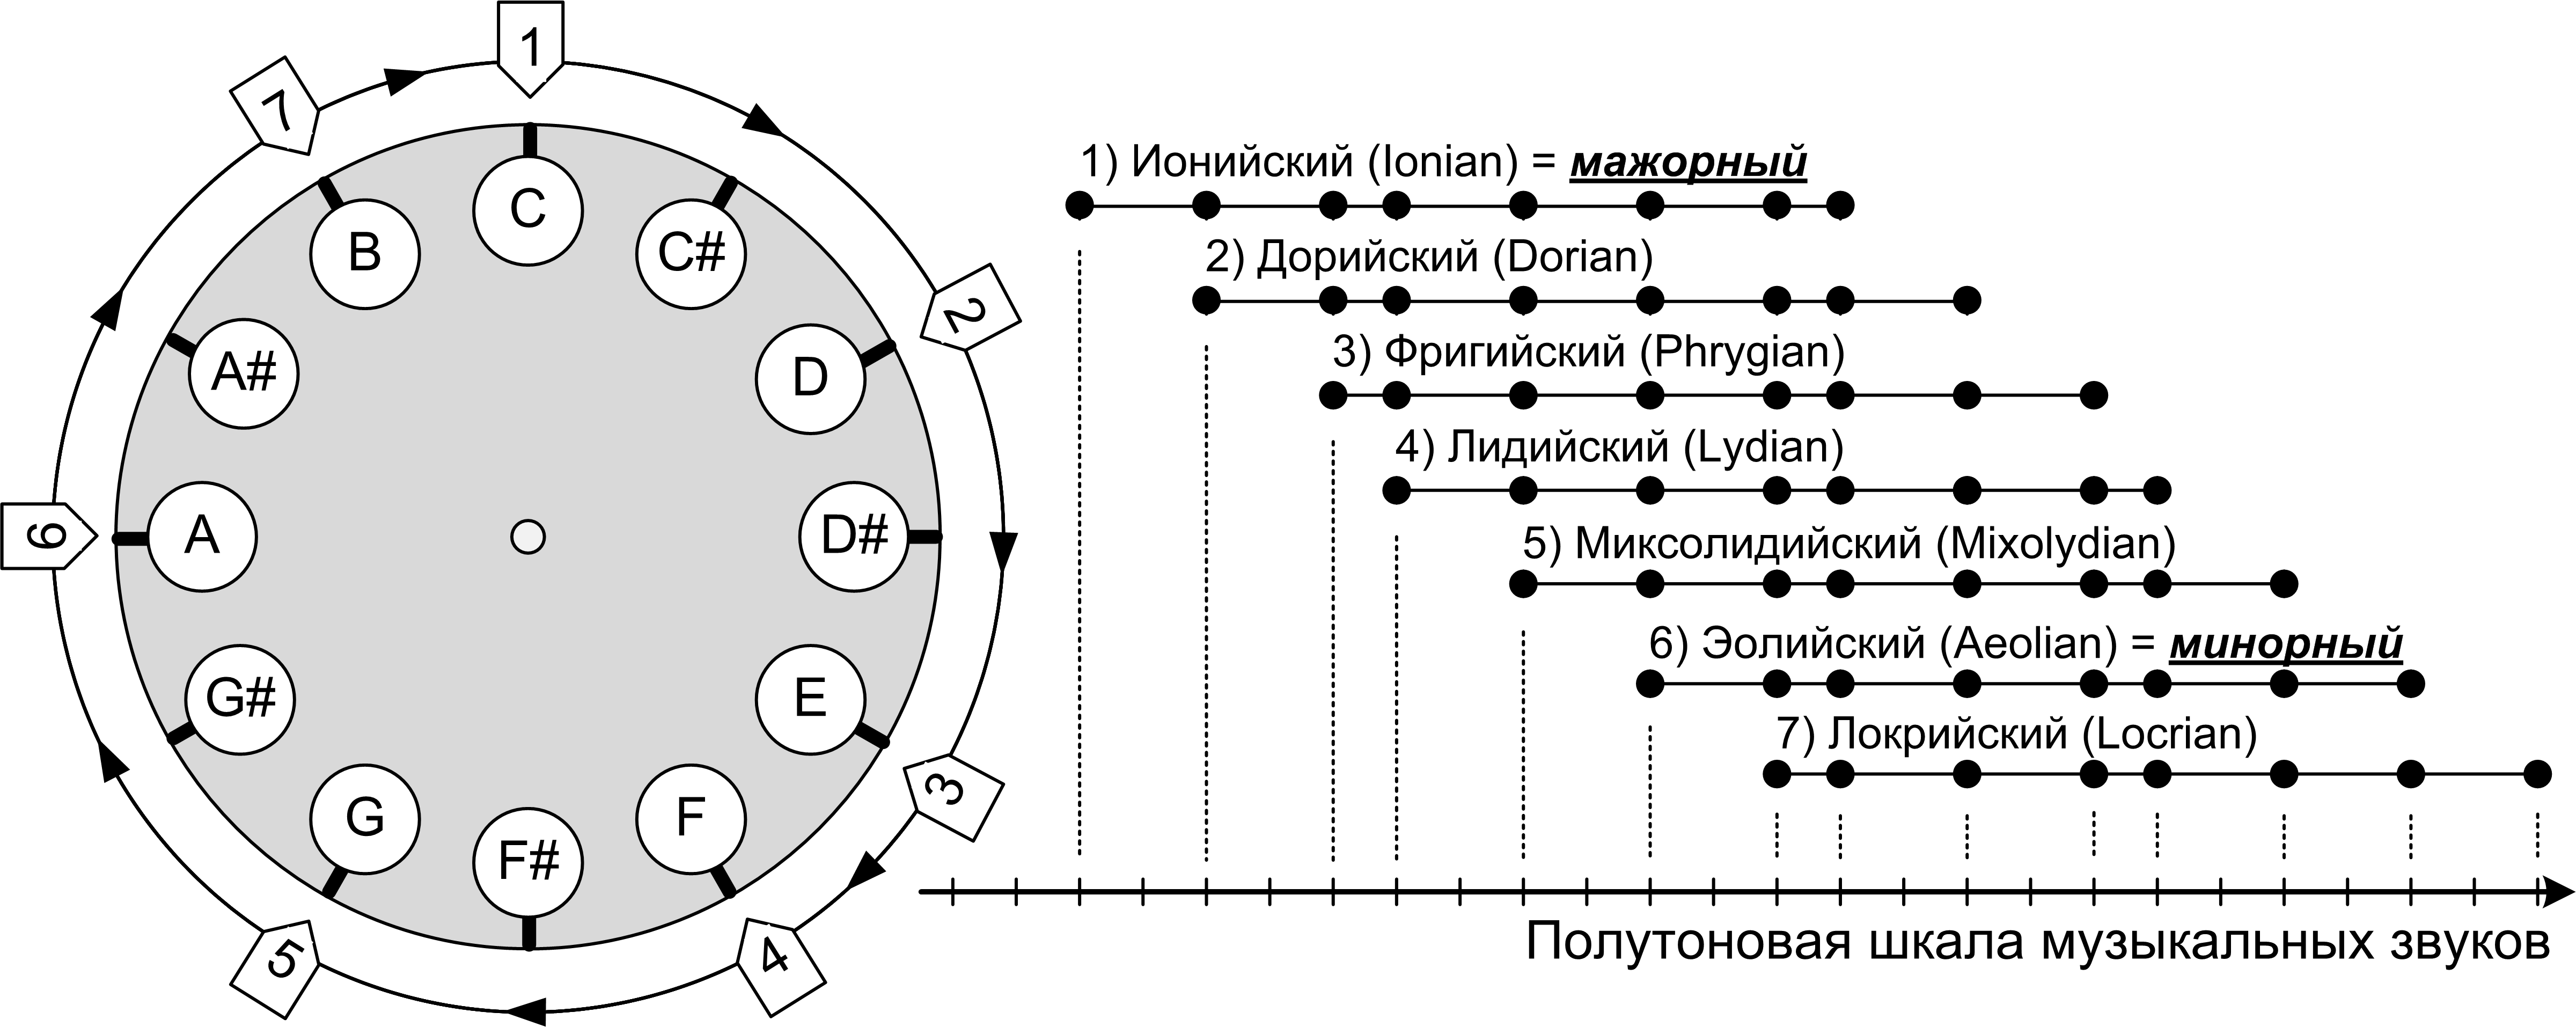
\includegraphics[width=\textwidth]{fig/intervals/modes} 
    \caption{Интервальная структура диатонических ладов}\label{fig:harmony:lad:modes}
\end{figure} 

<<Лидийский>> лад активно используется в джазовой музыке. Если вы хотите послушать <<ФА-лидийскую>> гамму, то достаточно сыграть:
\begin{center}
    ФА, СОЛЬ, ЛЯ, СИ, ДО, РЕ, МИ, ФА, МИ, РЕ, ДО, СИ, ЛЯ, СОЛЬ, ФА
\end{center}

То же самое в латинских обозначениях нот:
\begin{center}
    F, G, A, B, C, D, E, F, E, D, C, B, A, G, F
\end{center}
 
Построенная от ноты ФА(F), <<ФА-лидийская>> тональность содержит (как видно из рисунка \ref{fig:harmony:lad:modes}) ноты без диезов и бемолей. Кстати, этот лад для мелодий, дарящих ощущение счастья.


\paragraph{Пентатоника.} Пентатоника --- это тоже лад, но имеющий только 5-ступеней. То есть пентатоника из 12 нот октавы выделяет только 5 <<правильных>>, из которых можно составлять мелодию. Аналогично 7-ступенным ладам, получают 5 вариантов ладов с различными названиями, см. рисунок \ref{fig:harmony:lad:pentatonic}.

\begin{figure}[!ht]
    \centering
    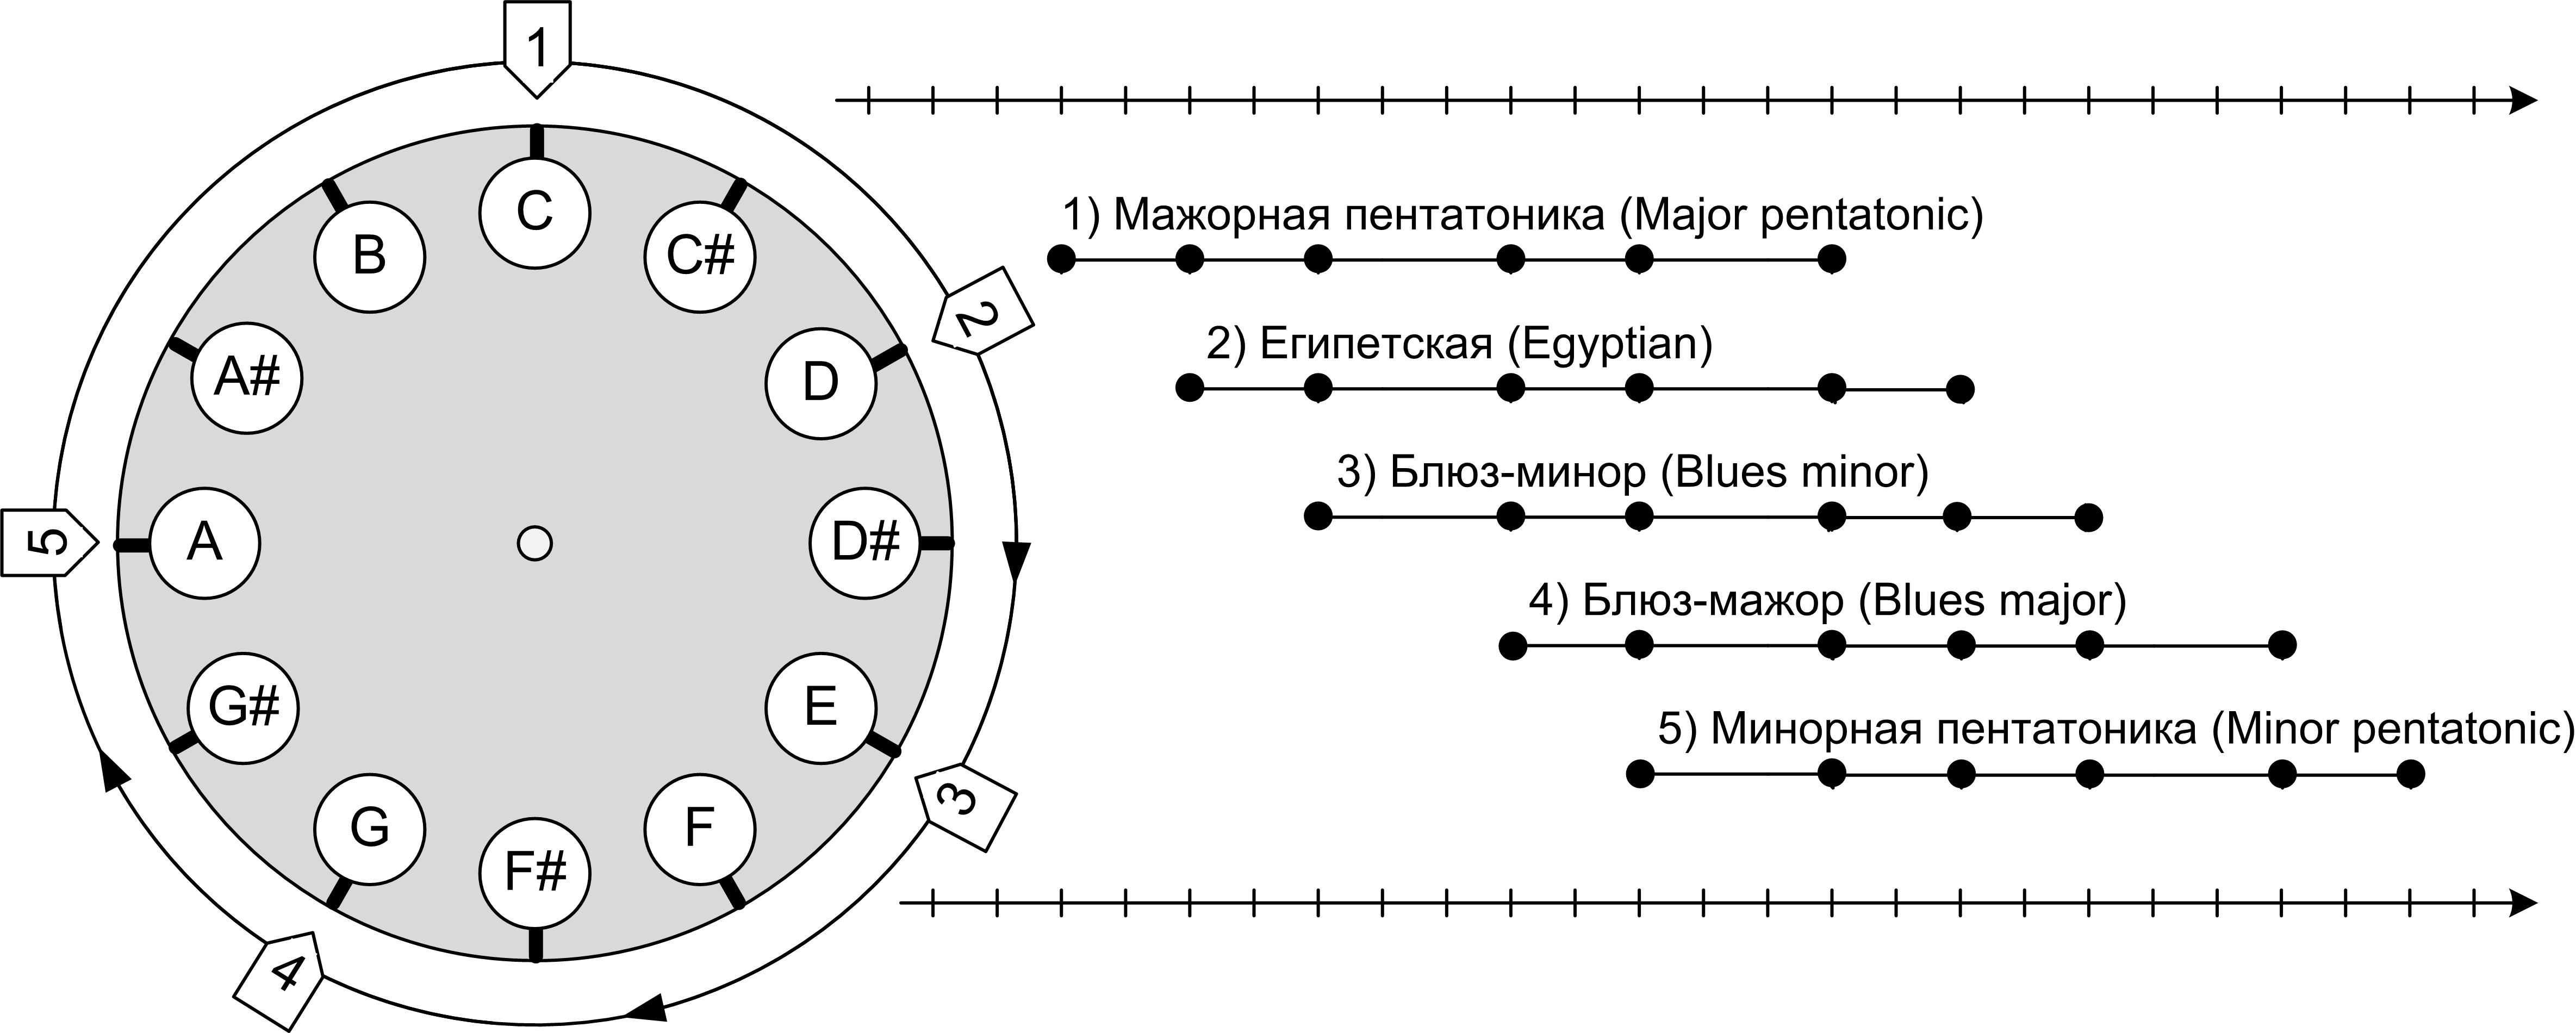
\includegraphics[width=\textwidth]{fig/intervals/pentatonic} 
    \caption{Интервальная структура пентатоники}\label{fig:harmony:lad:pentatonic}
\end{figure} 

Соответственно, например, интервальная структура мажорной пентатоники в полутонах:
\[
    \texttt{2-2-3-2-3}
\]

Обратите внимание, что пять ступеней пентатоники полностью содержатся в семиступенной структуре. Сравните рисунки \ref{fig:harmony:lad:pentatonic} и \ref{fig:harmony:lad:modes} и убедитесь, что пентатонику из диатоники можно получить, <<выкинув>> 4-ю и 7-ю отметки на октаве диатонических ладов.


%TODO: гамма лада в основных нотах

\section{Гаммы? Импровизация в жестких рамках}
\label{ch:harmony:scales}

Мы уже разобрались с тем, что такое лад, тональность и гамма в разделе \ref{ch:harmony:lad}. Вкратце, гамма --- это последовательно сыгранные ступени лада, отложенного от <<базовой>> ноты (тоники). Или, например, гамма --- это последовательно сыгранные ступени тональности.

Зачем играть гаммы?
\begin{itemize}
    \item Гамма приятно звучит, никакого дискомфорта, так почему бы и не сыграть?
    \item Начинающим полезно играть гаммы, проговаривая входящие ноты вслух, чтобы лучше запомнить их положение на грифе гитары.
    \item Гаммы --- это неплохая тренировка для пальцев. Даже профи, знающие множество простеньких пьес, чтобы разыграться перед выступлением, не гнушаются гаммами.
    \item Так как гамма --- это конкретный вариант \emph{лада}, то в каком порядке не играй ноты гаммы --- будет МУЗЫКА. Расслабьтесь, комбинируйте, играйте с длительностью, акцентами, импровизируйте. В конце концов музыка должна приносить удовольствие даже на этапе обучения!
\end{itemize}

Итак, ноты нотами, а играть-то нужно ручками. Поэтому на первых этапах придется потратить время на то, чтобы соотнести ноты с постановкой и движениями рук. Для гитары вопрос нот сводится к постановке пальцев левой\footnote{Если левши внимательно читали примечания, то они знают, что автор надеется, что они знают, что делать} руки на грифе. 

\begin{Definition}[Аппликатура]
    \emph{Аппликатура}\footnote{От латинского applico --- прикладываю, прижимаю} --- порядок расположения и чередования пальцев при игре на музыкальном инструменте.
\end{Definition}

Чтобы задать аппликатуру, гитаристы обычно пользуются изображением участка грифа, на котором точками отмечены места прижатия струн, а при необходимости возле точки указан и номер прижимающего пальца левой руки. Такой рисунок называется \emph{аппликатурным боксом}. Пальцы левой руки принято нумеровать слеюдующим образом:
\begin{itemize}
    \item указательный --- 1;
    \item средний --- 2;
    \item безымянный --- 3;
    \item мизинец --- 4.
\end{itemize}

Большой палец левой руки не нумеруется, ибо находится с тыльной стороны грифа и оказывает только моральную поддержку остальным пальчикам, имеющим дело со струнами.

Итак, нам уже известно, что только диатонических ладов (включающих мажор и минор) семь штук, пентатоник --- пять. Так что имеется большой выбор в каком ладу поиграть. А о тональностях и говорить нечего --- смело умножайте количество ладов на 12!

Давайте ограничимся только гаммой ДО-мажор. При желании с остальными вы разоберетесь по аналогии. Не надо думать, что нужно уметь играть гаммы во всех ладах и тональностях. Вы же не робот! А если робот, то вот неплохое чтиво\footnote{Признанным специалистом в области гамм является Андреас Сеговия, чьи гаммы играет не первое поколение классических гитаристов. Открыв его книжку \cite{bib:segovia:Scales} можно увидеть 9 страниц нотной записи гамм (с аппликатурными пометками) во всех тональностях мажорного и минорного ладов. Эта книжка --- справочник, методичка, её с ужасом открывает на нужной странице бедный ученик музыкальной школы, терзает заданную учителем гамму, и с ужасом закрывает обратно, чтобы навсегда о ней забыть. Через несколько десятков лет, ставший профессионалом ученик, возможно и откроет книжку Сеговии, чтобы подглядеть как ставил на струны свои гениальные пальцы маэстро. Из любопытства. И только потому, что сам ужасно много знает}: \cite{bib:segovia:Scales} справочник от гениального гитариста и педагога Андреаса Сеговии.

\begin{Example}[Гамма ДО-мажор на одной струне]
    \label{ex:harmony:scales:d:maj}
    
    Нота ДО находится на первом ладу второй струны\footnote{Стандартный, МИ-СИ-СОЛЬ-РЕ-ЛЯ-МИ, строй}. Последовательно зажимайте на второй струне указательным пальцем левой руки лады 1-й, 3, 5, 6, 8, 10, 12, 13 и одновременно с этим защипывайте правой рукой вторую струну. Прозвучит гамма ДО-мажор. От ноты ДО первой октавы до ноты ДО второй октавы. 
    
    Делаем выводы.
    \begin{itemize}
        \item Неудобно: сдвиг руки вдоль по грифу --- слижком грубое движение, о быстрой игре можно забыть.
        \item Неэкономно: музыка --- не спорт, а если так махать руками, то понадобится допинг.
        \item Непрактично: возможности гитары не используются в полной мере, ведь нужные ноты можно найти поблизости --- на соседних струнах.
    \end{itemize}
\end{Example}

Два экономных варианта исполнения гаммы ДО-мажор приведены на рисунке \ref{fig:harmony:scales:c:dur1}. Левая рука двигается только поперек грифа и каждый палец отвечает только за свой лад. Аппликатура слева --- гамма в одну октаву, а спрва --- двухоктавная гамма. В серых кружочках --- местах прижатия струны, написано латинское обозначение ноты, а не номер пальца (так как пальцы вдоль грифа не сдвигаются, то в этом нет необходимости). Стрелочками показан порядок постановки пальцев на струны при игре <<по восходящей>> --- дойдя до конца, играйте в обратной последовательности.

\begin{figure}[!ht]
    \centering
    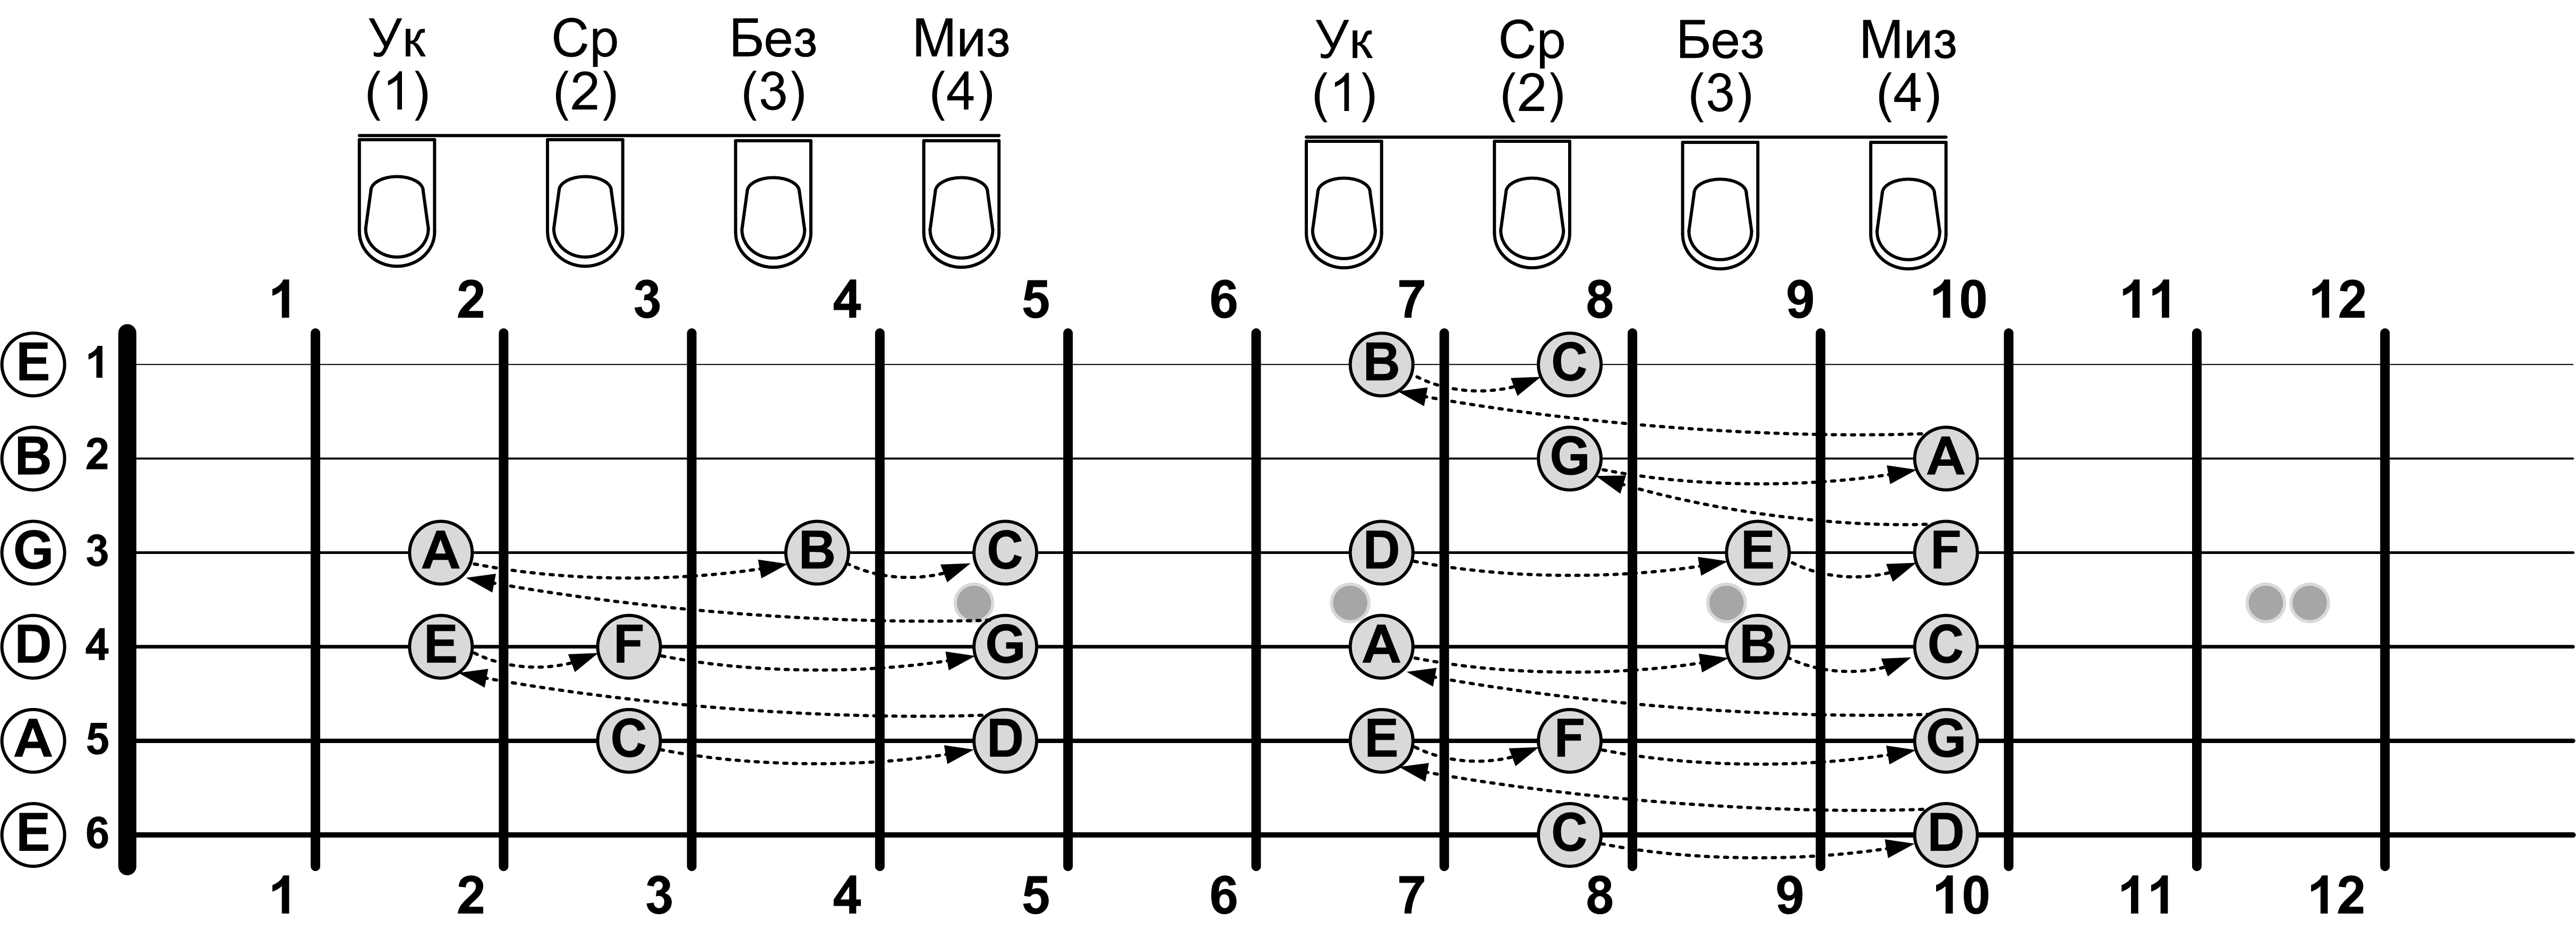
\includegraphics[width=\textwidth]{fig/intervals/c-dur-csale-1} 
    \caption{Два варианта аппликатур гаммы ДО-мажор}\label{fig:harmony:scales:c:dur1}
\end{figure} 

Стоит отметить, что во время испольнения не следует снимать (поднимать над грифом) раньше времени пальцы, которые можно оставить\footnote{Это принцип экономии: не делай лишних движений, расслабь и оставь на месте палец, который не нужно двигать. Новичку, пока нет растяжки и независимости в пальцах левой руки, это будет трудно: поднимаешь один палец, а за ним сам собой поднимается второй. Так что на начальных этапах этим правилом (а куда деваться?) придется пренебрегать. Пройдет время, организм поймет куда нужно эволюционировать и вы почувствуете, как экономность движений доставляет удовольствие}

Если внимательно поискать на грифе места (рисунок \ref{fig:guitar:notes-on-grip} в помощь), где еще можно сыграть гамму ДО-мажор не растопыривая пальцы слишком широко и не смещаясь вдоль грифа, то можно найти вариант, представленный на рисунке \ref{fig:harmony:scales:c:dur2}.

\begin{figure}[!ht]
    \centering
    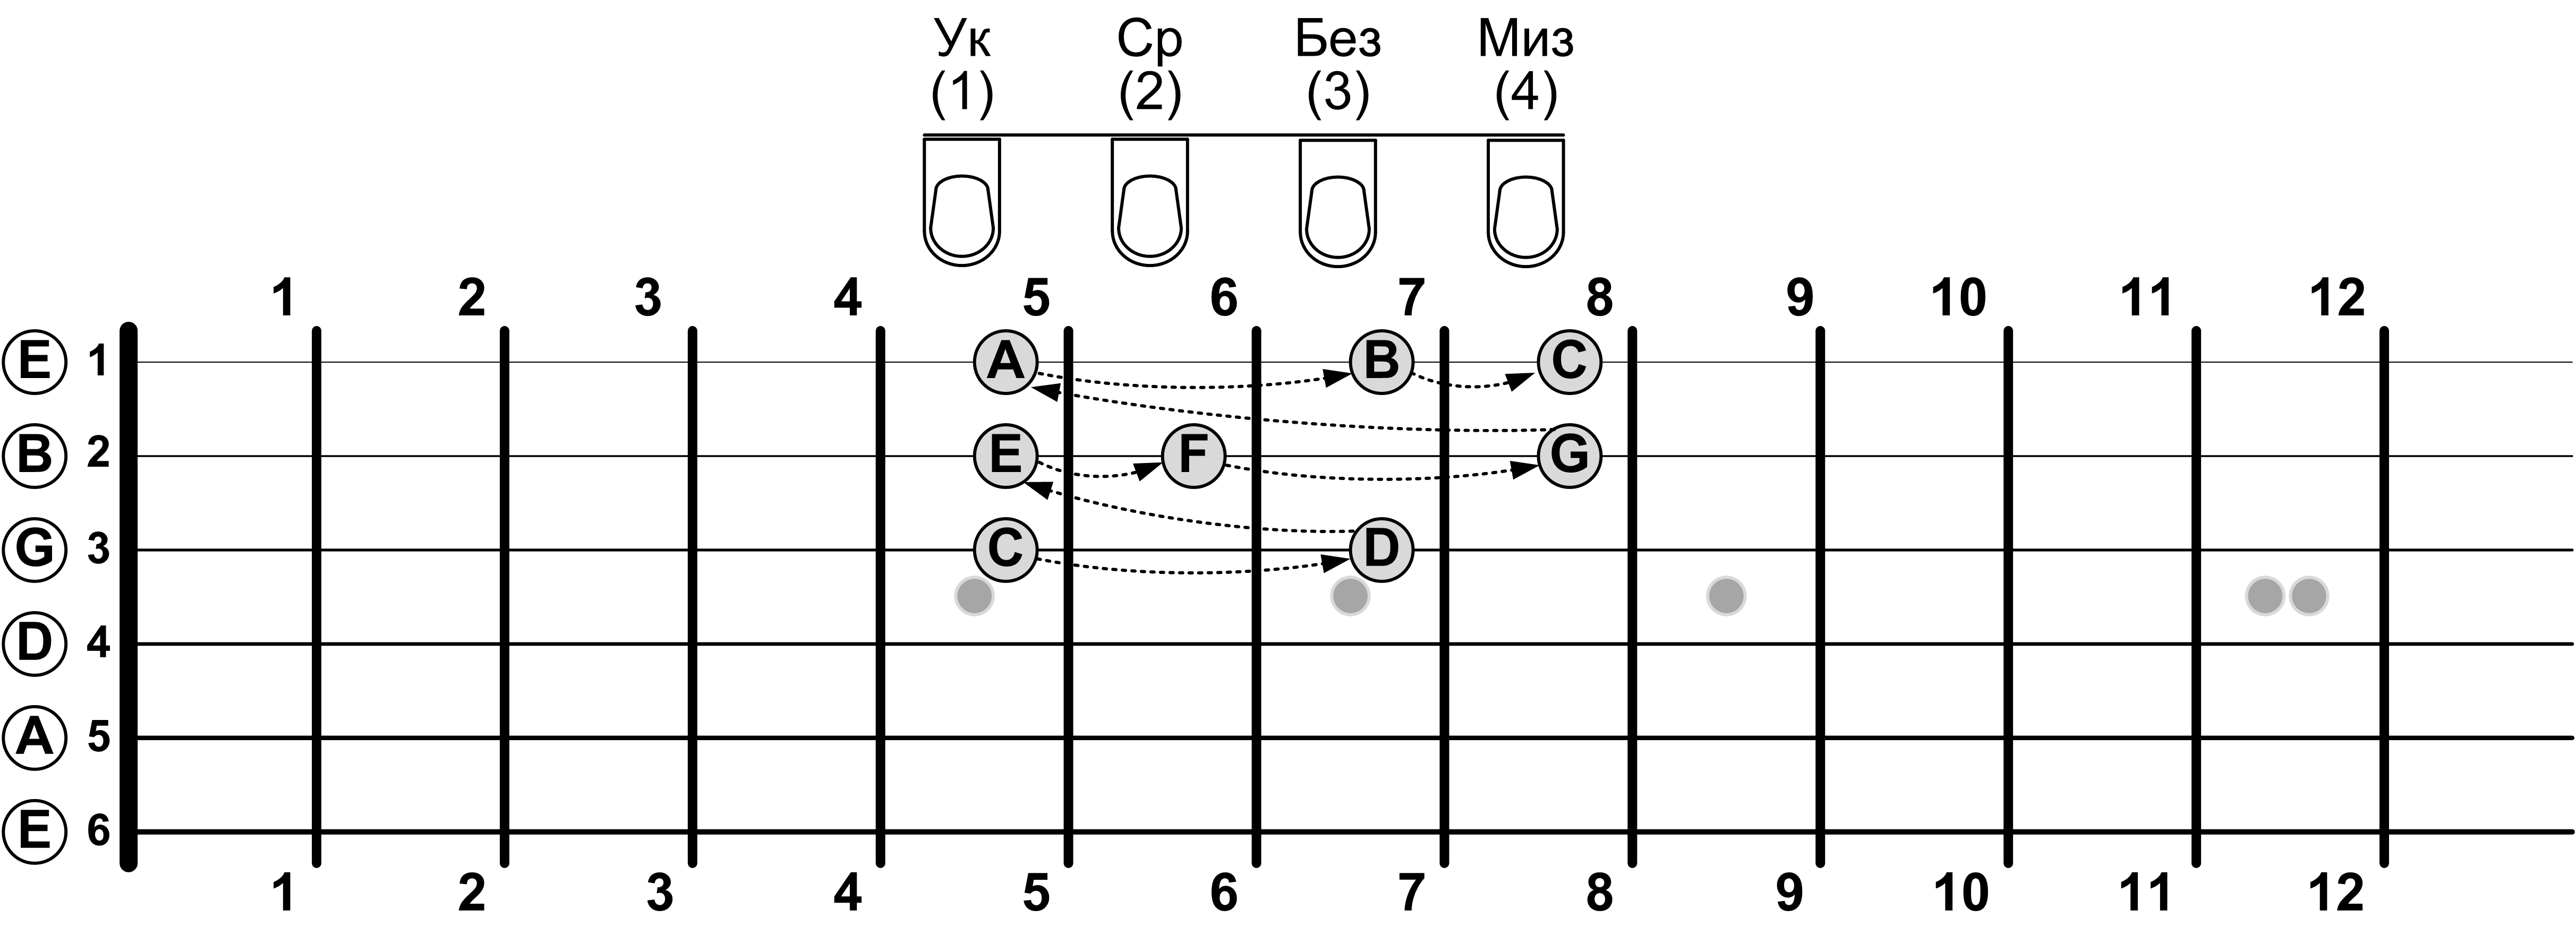
\includegraphics[width=\textwidth]{fig/intervals/c-dur-csale-2} 
    \caption{Аппликатура гаммы ДО-мажор длиной в одну октаву}\label{fig:harmony:scales:c:dur2}
\end{figure} 

Но смещаться по грифу на практике все-таки придется. Вариант двухоктавной гаммы ДО-мажор от Андреаса Сеговии приведен на рисунке \ref{fig:harmony:scales:c:dur:segovia}. В кружках, как и положено, написаны номера прижимающих пальцев левой руки. Фрагменты этого аппликатурного шаблона вы можете увидеть по-отдельности на рисунках \ref{fig:harmony:scales:c:dur1} и \ref{fig:harmony:scales:c:dur2}. На третьей струне придется испытать неудобства: после того, как 3-м пальцем на 4-м ладу сыграна нота СИ(B), нужно быстро и точно переставить (или <<съехать>>, если струна гладкая) кисть так, чтобы указательный палец встал на 5-й лад (ноту ДО(C)) --- дальше продолжаем в экономном режиме, как на рисунке \ref{fig:harmony:scales:c:dur2}.

\begin{figure}[!ht]
    \centering
    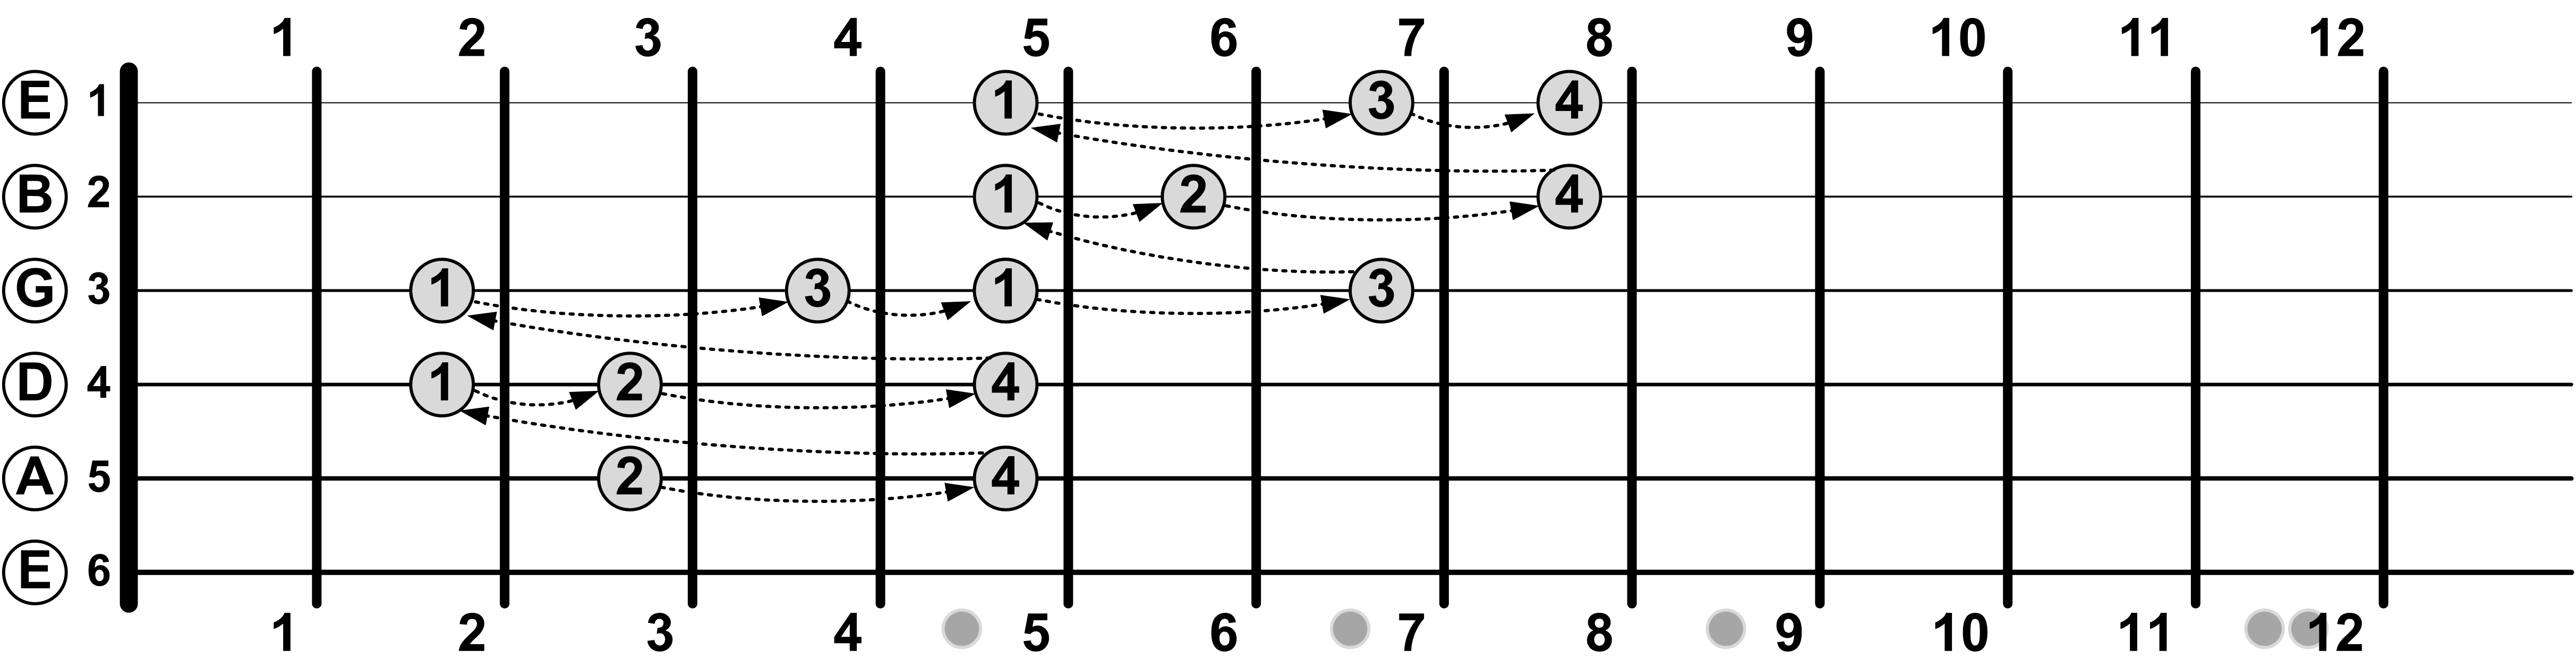
\includegraphics[width=\textwidth]{fig/intervals/c-dur-csale-segovia} 
    \caption{Аппликатура двухоктавной гаммы ДО-мажор}\label{fig:harmony:scales:c:dur:segovia}
\end{figure} 

А теперь небольшой бонус: вы научились играть не только варианты гаммы ДО-мажор. Сдвиньте, например, кисть на два лада вниз по грифу и сыграйте то, что помнят ваши руки. Вуаля: вы сыграли гамму РЕ-мажор!

Когда вы научитесь играть гамму ДО-мажор хотя бы в двух октавах (см. раздел \ref{ch:harmony:scales}) и запомните, где находятся на грифе 7-нот ДО-мажорной гаммы, то вы легко сыграете характерные гаммы для любого из перечисленных ладов в <<основных нотах>>, опираясь на известные аппликатуры ДО-мажорной гаммы. Достаточно лишь начать с нужной ноты и, в случае пентатоники, пропускать ненужные. Сверьтесь с рисунками \ref{fig:harmony:lad:modes} и \ref{fig:harmony:lad:pentatonic} и убедитесь:
\begin{itemize}
    \item Диатоника:
    \begin{itemize}
        \item Ионийский (мажорный) лад. Гамма ДО-мажор: <<C,D,E,F,G,A,B,C>>.
        \item Дорийский лад. РЕ-Дорийская гамма: <<D,E,F,G,A,B,C,D>>.
        \item Фригийский. МИ-Фригийская гамма: <<E,F,G,A,B,C,D,E>>.
        \item Лидийский. ФА-Лидийская гамма: <<F,G,A,B,C,D,E,F>>.
        \item Миксолидийский. СОЛЬ-Миксолидийская гамма: <<G,A,B,C,D,E,F,G>>.
        \item Эолийский (минорный). Гамма ЛЯ-минор: <<A,B,C,D,E,F,G,A>>.
        \item Локрийский. СИ-Локрийская гамма: <<B,C,D,E,F,G,A,B>>.
    \end{itemize}

    \item Пентатоника:
    \begin{itemize}
        \item Мажорная пентатоника. ДО-мажорная гамма: <<C,D,E,G,A,С>>.
        \item Египетская пентатоника. РЕ-Египетская гамма: <<D,E,G,A,C,D>>.
        \item Блюз-минор. МИ-блюз-минорная гамма: <<E,G,A,C,D,E>>.
        \item Блюз-мажор. СОЛЬ-блюз-мажорная гамма: <<G,A,C,D,E,G>>.
        \item Минорная. ЛЯ-минорная гамма: <<A,C,D,E,G,A>>.
    \end{itemize}
\end{itemize}

Ого! И все это на основе одной гаммы! А теперь представьте, что получившийся аппликатурный шаблончик можно сдвинуть вдоль грифа! Любой лад почти в любой тональности! Фантастика. Еще раз подтверждаем тезис, что музыкальная теория сложнее практики.

Справедливости ради нужно отметить, что если вы стали фанатом какого-либо лада, то можно посидеть над грифом гитары или над рисунком \ref{TODO} и разработать наиболее эффективный аппликатурный бокс для игры в любимой тональности.



%TODO: голос? у музыки есть голос?

\section{Чем больше звуков, тем лучше? Аккорды}
\label{ch:harmony:chords}

Из раздела \ref{ch:harmony:interval} вы узнали, что \emph{интервал} для физиков --- это \emph{мера расстояния} между двумя звуками, а для лириков --- это \emph{два звука}, сыгранных одновременно или друг за другом.

Аккорд же --- понятие целиком лирическое.

\begin{Definition}[Аккорд]
    \emph{Аккорд} --- это три или более музыкальных звука, извлеченных (звучащих) одновременно.
\end{Definition}

Видели ведь, наверное, как играют <<боем>>? Правая рука ходит вверх-вниз, и ритмично бьет по всем струнам одним или несколькими пальцами. Говорить о том, что звуки извлекаются одновременно не приходится --- струны задеваются одна за другой, но так как это происходит достаточно быстро, то \emph{звучат} они некоторое время все вместе и мы слышим \emph{аккорд}.

Какие же звуки должны входить в аккорд, чтобы он звучал гармонично? Точно не любые. Есть ли правила построения аккордов?

Да, система аккордов сложилась и давно устоялась. В основе этой системы лежат мажорный и минорный лады, и она определяет интервальную структуру аккордов и правила их именования. Кстати, поэтому аккорды делятся на две большие группы: мажорные (веселые) и минорные (грустные).

TODO

% интервальная структура аккорда и названия
% как декодировать этот шифр --- обозначения аккордов?

% TODO: струн шесть - звука три
% пример аппликатурного бокса

% ходовые аккорды в первой позиции

% аппликатуры простейших аккордов, которые можно унести с баррэ в любое место грифа.



\section{Так квинтовый или квартовый? Квинто-квартовый круг}
\label{ch:harmony:kvinto-kvarto-round}

На самом деле полное название этого полезного помошника, которго легко сделать из бумаги: <<квинто-квартовый круг мажорных и минорных тональностей>>. Выглядит он странно: см. рисунок \ref{fig:harmony:kvinto-kvarto:kvinto-kvarto-final}. И хотелось бы не только научиться им пользоваться, но и понять почему он именно такой.

Круг может помочь, если вы хотите:
\begin{itemize}
    \item Подобрать <<сочетающиеся>> аккорды для аккомпанемента песен.
    
    \item Определить, какие ноты входят в ту или иную мажорную или минорную тональность.
    
    \item Сменить <<тональность>> аккомпанемента песни. Человеческим языком: \emph{каждую} ноту исходной тональности нужно повысить или понизить на заданное количество полутонов. Зачем? Чтобы было удобнее петь. При этом интервальная структура (т.е. характер, например, веселый или грустный) музыки не изменится, а произведение <<в целом>> будет звучать ниже или выше, <<подстраиваясь>> таким образом под голос исполнителя.    

    \item Решить <<академические>> задачки, например, определить тональность произведения по нотам или определить параллельную тональность.
    
    \item И много чего ещё\ldots
\end{itemize}

Мы не будем сейчас учиться как решать эти задачки, мы начнем разбираться с устройством круга. А в процессе станет понятно не только, как решать эти задачки, но и многое другое.

Глядя на рисунок \ref{fig:harmony:interval:octave-kon-dis} можно увидеть, что для отдельно взятого звука в пределах октавы существует лишь \emph{два} звука, образующий с исходным звуком совершенный консонанс. Относительно исходного эти звуки находятся на расстоянии в 5 (кварта) и 7 (квинта) полутонов. Оказывается, что можно переупорядочить ноты так, чтобы совершенные консонансы стали соседями исходного звука: один справа, другой слева!

Начнём, например с ноты ДО, и отступая по семь полутонов по часовой стрелке:
\[
    C\rightarrow 
    G\rightarrow 
    D\rightarrow 
    A\rightarrow 
    E\rightarrow 
    B\rightarrow 
    {F\sharp}\rightarrow
    {C\sharp}\rightarrow
    {G\sharp}\rightarrow
    {D\sharp}\rightarrow
    {A\sharp}\rightarrow
    F\rightarrow 
    C
\]
замкнем круг и получим результат, представленный на рисунке \ref{fig:harmony:kvinto-kvarto:kons-rearrange}.

\begin{figure}[!ht]
    \centering
    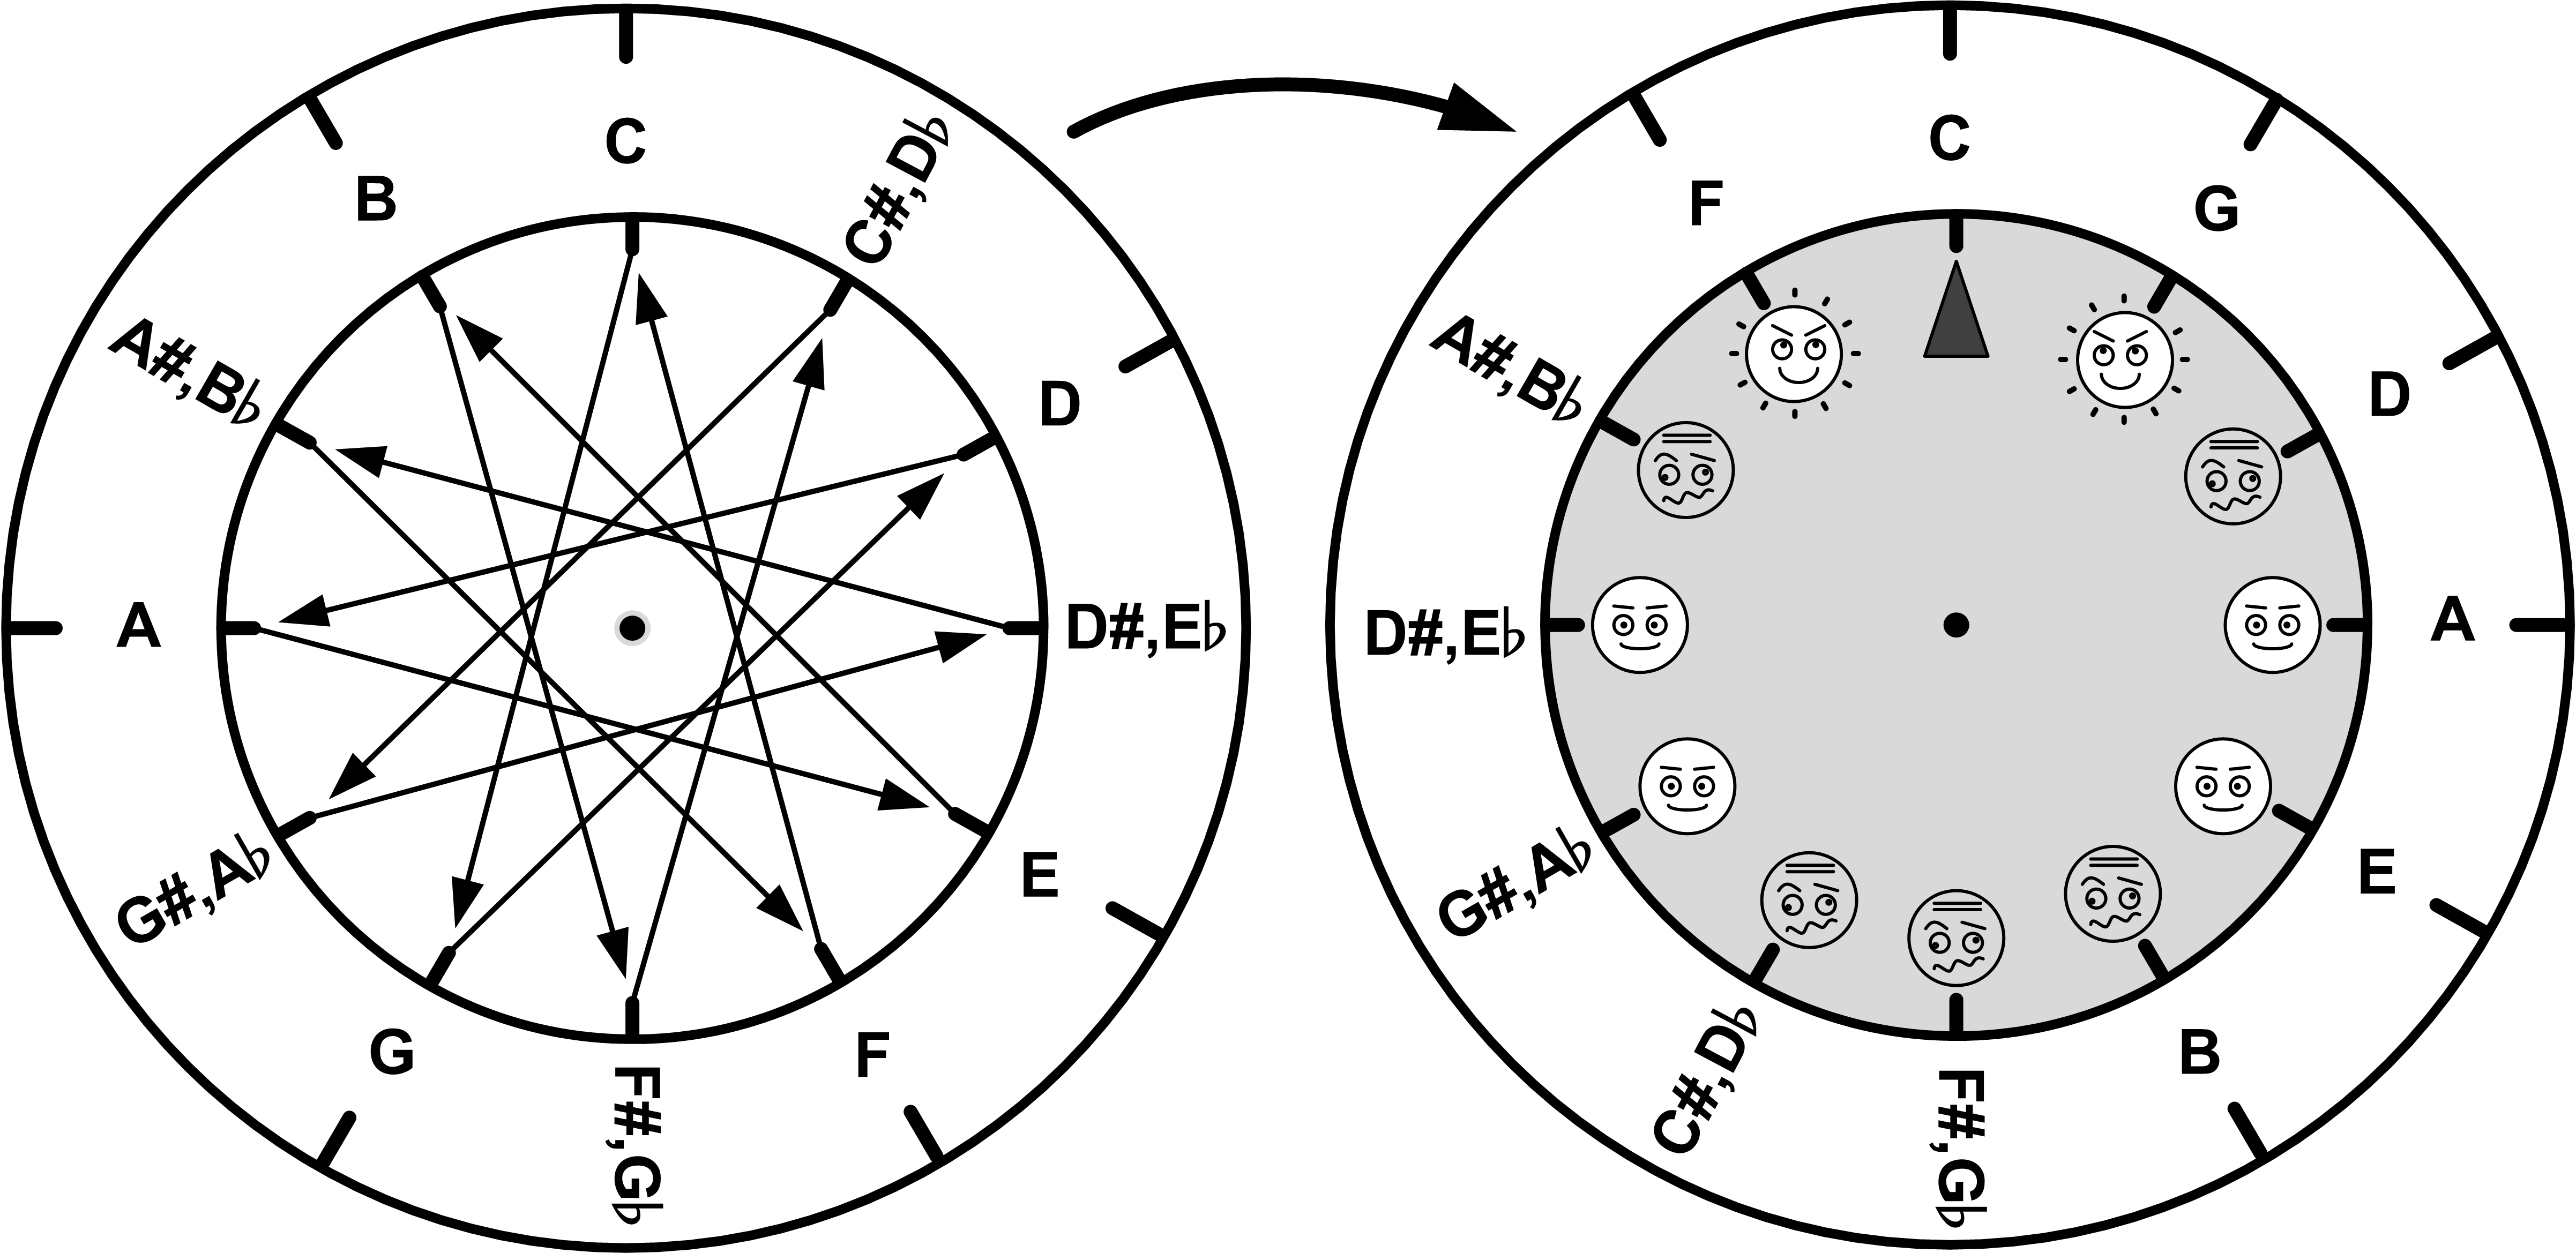
\includegraphics[scale=0.7]{fig/kvinto-kvarto/kons-rearrange} 
    \caption{Консонансы по соседству}\label{fig:harmony:kvinto-kvarto:kons-rearrange}
\end{figure} 

Теперь достаточно ткнуть в любую ноту на получившемся круге и узнать её совершенные консонансы: соседом против часовой стрелки будет совершенный консонанс на расстоянии 5 полутонов (чистая кварта), а по часовой --- консонанс на расстоянии 7 полутонов (чистая квинта). Например, возмьем ноту ЛЯ(A) и сразу определяем консонансы: РЕ(D) --- кварта от ЛЯ и МИ(E) --- квинта.

Обратите внимание на то, что среди переупорядоченных нот явно выделились две цепочки: цепочка нот без диезов и бемолей и цепочка нот со знаками альтерации. Конечно, это не случайность: ноты без диезов и бемолей --- это названия ступеней мажорного лада (а точнее --- тональность ДО-мажор). И само-собой, мажорный лад в своё время был сформирован с учетом расположения совершенных консонансов и вполне возможно, автор при этом глядел на полученный нами круг.

Итак, ноты тональности ДО-мажор выстроились в одну цепочку. При этом тоника --- ДО, идет в этой последовательности второй, если считать по часовой стрелке.

Таким образом упростилась задача определения нот для \emph{любой} мажорной тональности: 
\begin{enumerate}
    \item нужно отметить тонику на круге и отступить от нее на один сектор против часовой стрелки;
    \item включая полученную ноту, двигаясь по часовой стрелке, отсчитать семь нот тональности.
\end{enumerate}

Например, требуется определить ноты тональности РЕ-мажор (см. рисунок \ref{fig:harmony:kvinto-kvarto:d-maj}). Отступаем от $D$ против часовой стрелки, а затем по часовой собираем 7 нот:
\[
    G\rightarrow 
    D\rightarrow 
    A\rightarrow 
    E\rightarrow 
    B\rightarrow 
    {F\sharp}\rightarrow
    {C\sharp}
\]

\begin{figure}[!ht]
    \centering
    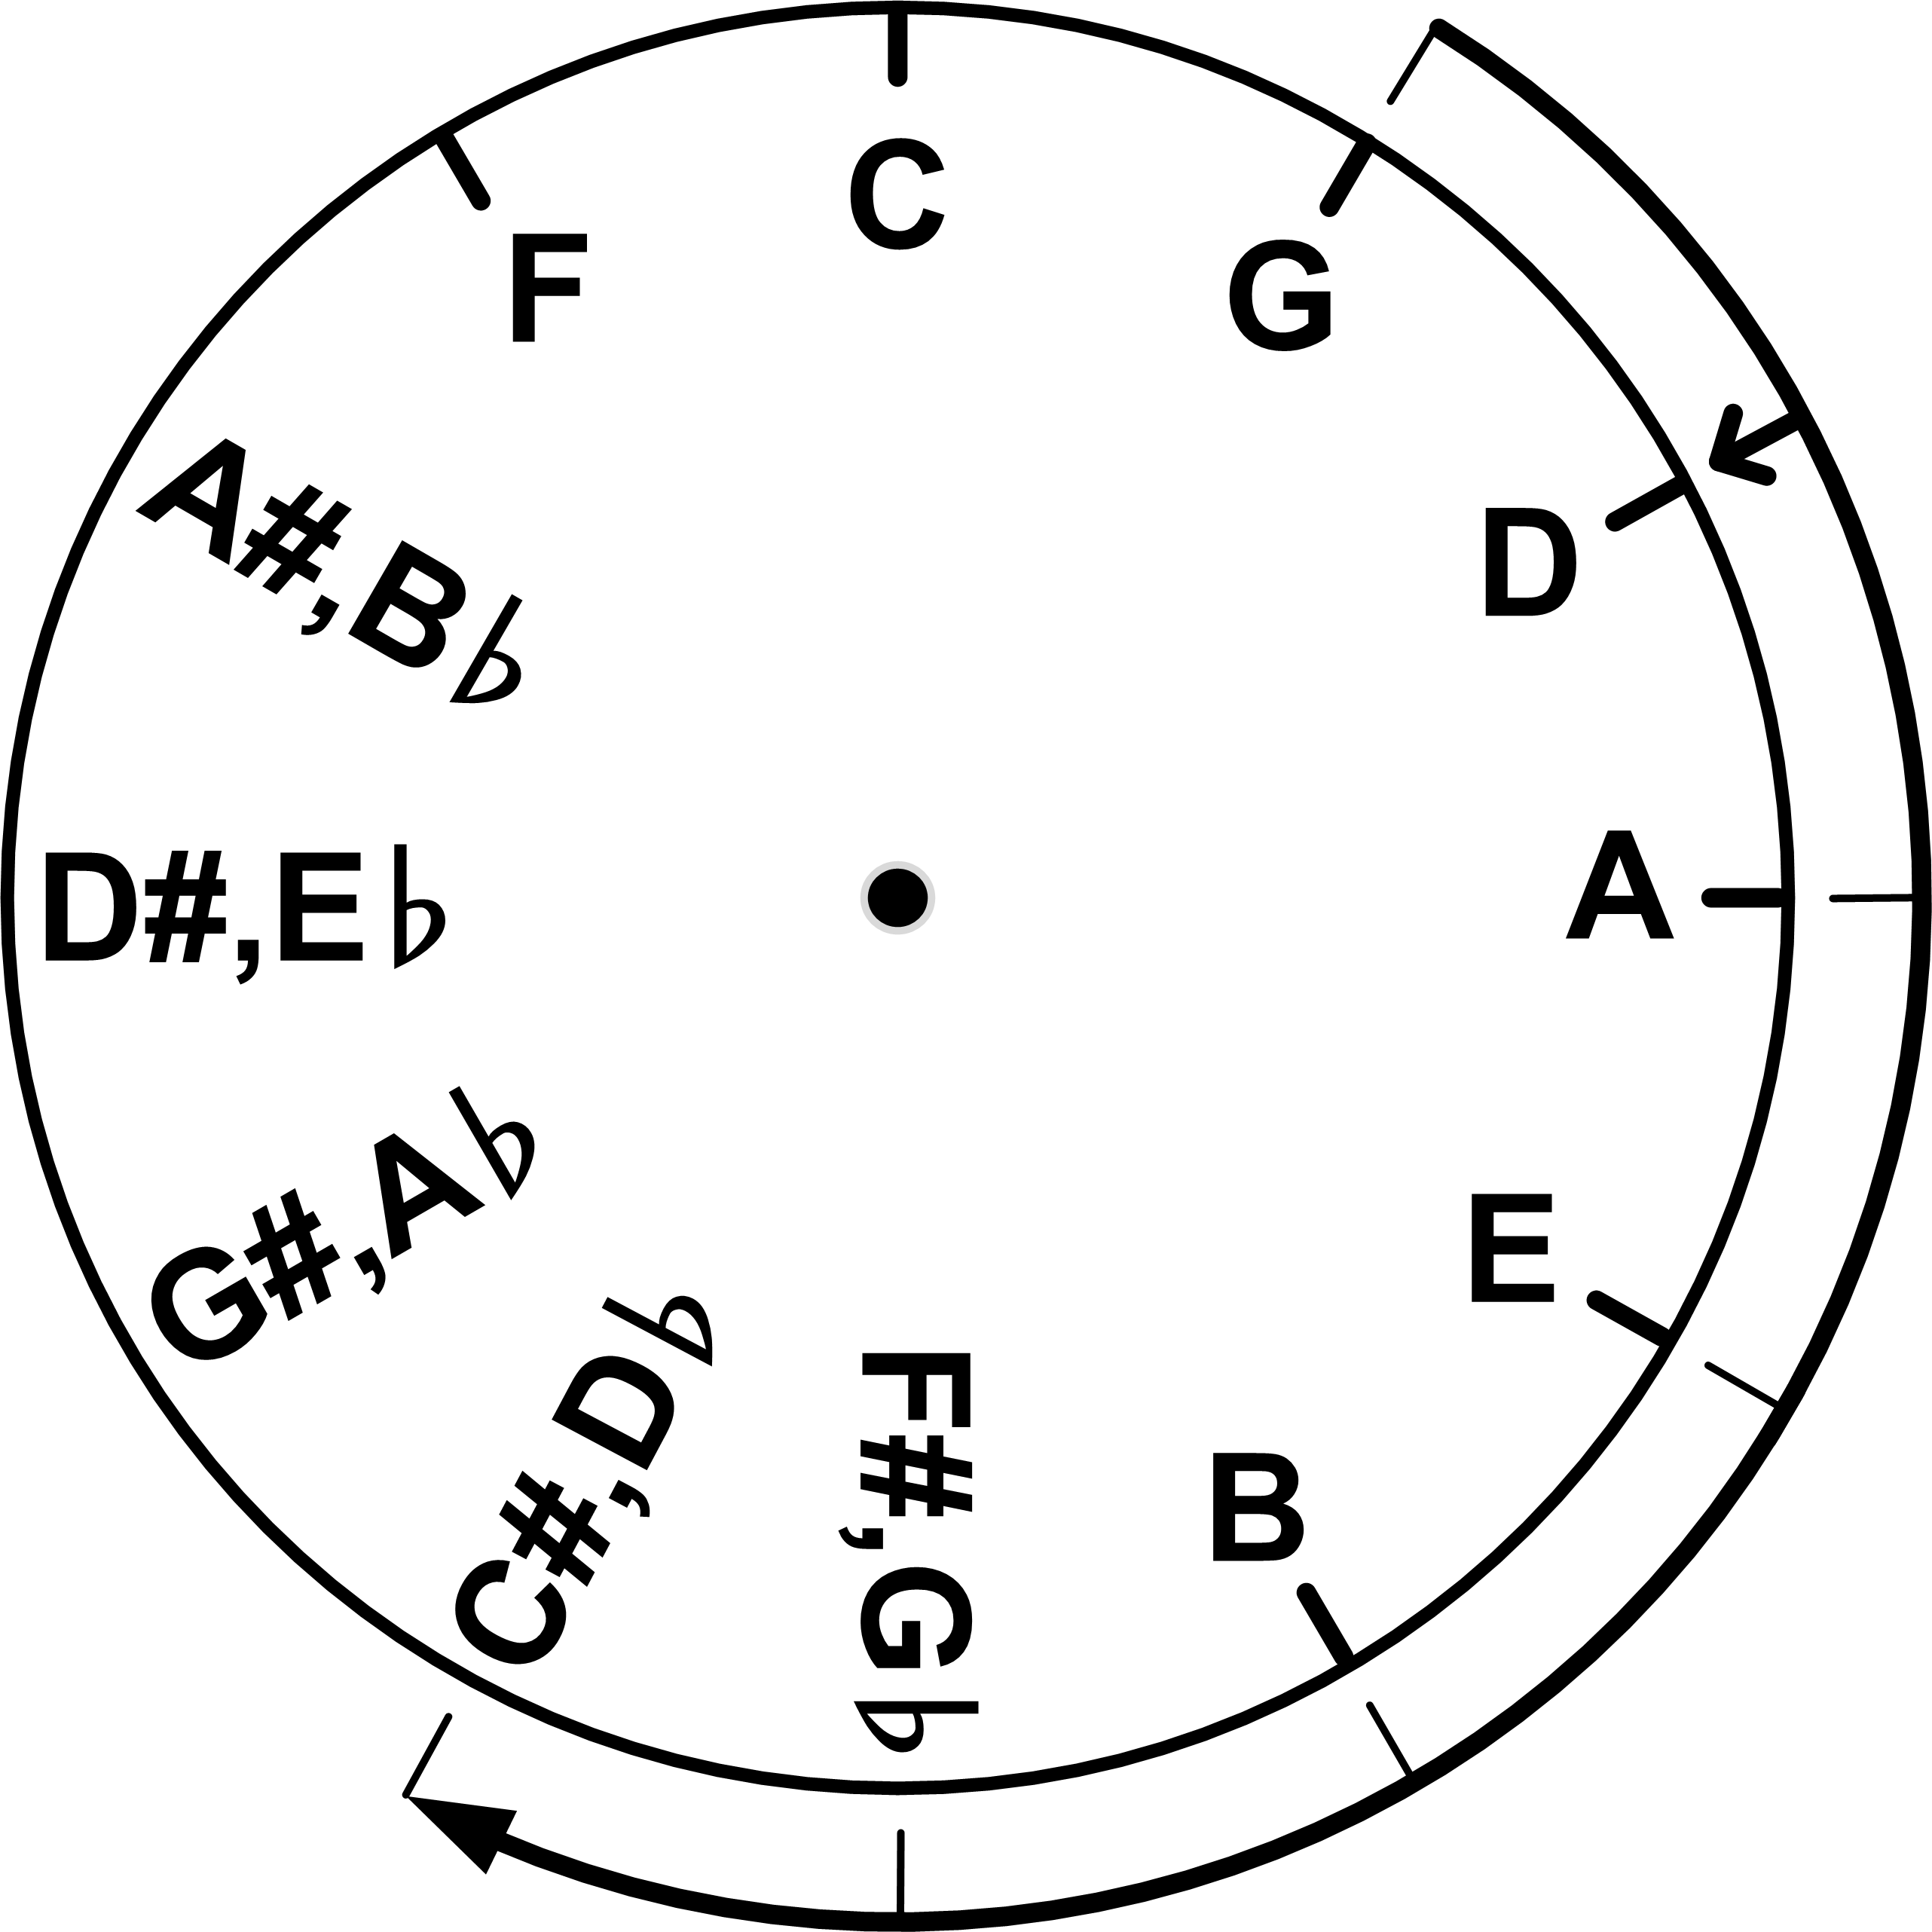
\includegraphics[scale=0.5]{fig/kvinto-kvarto/kvinto-kvarto-d-maj} 
    \caption{Ноты тональности $D$-maj}\label{fig:harmony:kvinto-kvarto:d-maj}
\end{figure}

Естественно, что ноты по высоте пока не упорядочены, но это совсем несложно сделать, зная, что тоника внизу:
\[
    D\rightarrow 
    E\rightarrow 
    {F\sharp}\rightarrow
    G\rightarrow 
    A\rightarrow 
    B\rightarrow 
    {C\sharp}
\]

Мы разобрались как определять ноты любой мажорной тональности. Как мы уже знаем, для любой мажорной тональности можно подобрать <<параллельную>> минорную тональность\footnote{Для тональности любого диатонического лада можно подобрать <<параллельную>> тональность из другого диатонического лада}. Напомню, что параллельные тональности состоят из одних и тех же нот, но отличаются тоникой --- самым низким звуком. Поэтому музыкальные звуки, соответствующие одинаковым нотам параллельных тональностей, могут иметь разное высотное положение, то есть находиться в разных октавах.

Мажорный и минорный лады --- фундамент музыки. Особенно они востребованы при составлении аккомпанемента к песням. Поэтому ограничиться шпаргалкой только для мажорного лада никак нельзя: нужно подключить и минорный\footnote{Кто внимательно читал раздел \ref{ch:harmony:lad}, тот знает, что, например, тональность ЛЯ-минор параллельна тональности ДО-мажор. Таким образом, отличие лишь в том, что тоника ЛЯ будет находится в последовательности нот без знаков альтерации (ДО-мажор) пятой по счету по часовой стрелке. Так что по имеющемуся на данный момент кругу уже можно определить ноты и для любой минорной тональности: отступаем пять секторов от тоники против часовой стрелки и собираем семь нот --- по часовой}.

Возьмем три круга (см. рисунок \ref{fig:harmony:kvinto-kvarto:minor-major-mapping}), и разобъем каждый их них на 12 равных секторов. На первом (самом большом) круге отметим 12 нот в их естественной последовательности; на втором (поменьше, на рисунке \ref{fig:harmony:kvinto-kvarto:minor-major-mapping} выделен серым цветом) --- отметим ступени мажорного лада; на третьем (самом маленьком) --- ступени минорного. Насадим все круги на общую ось, проходящую через центр каждого круга.

\begin{figure}[!ht]
    \centering
    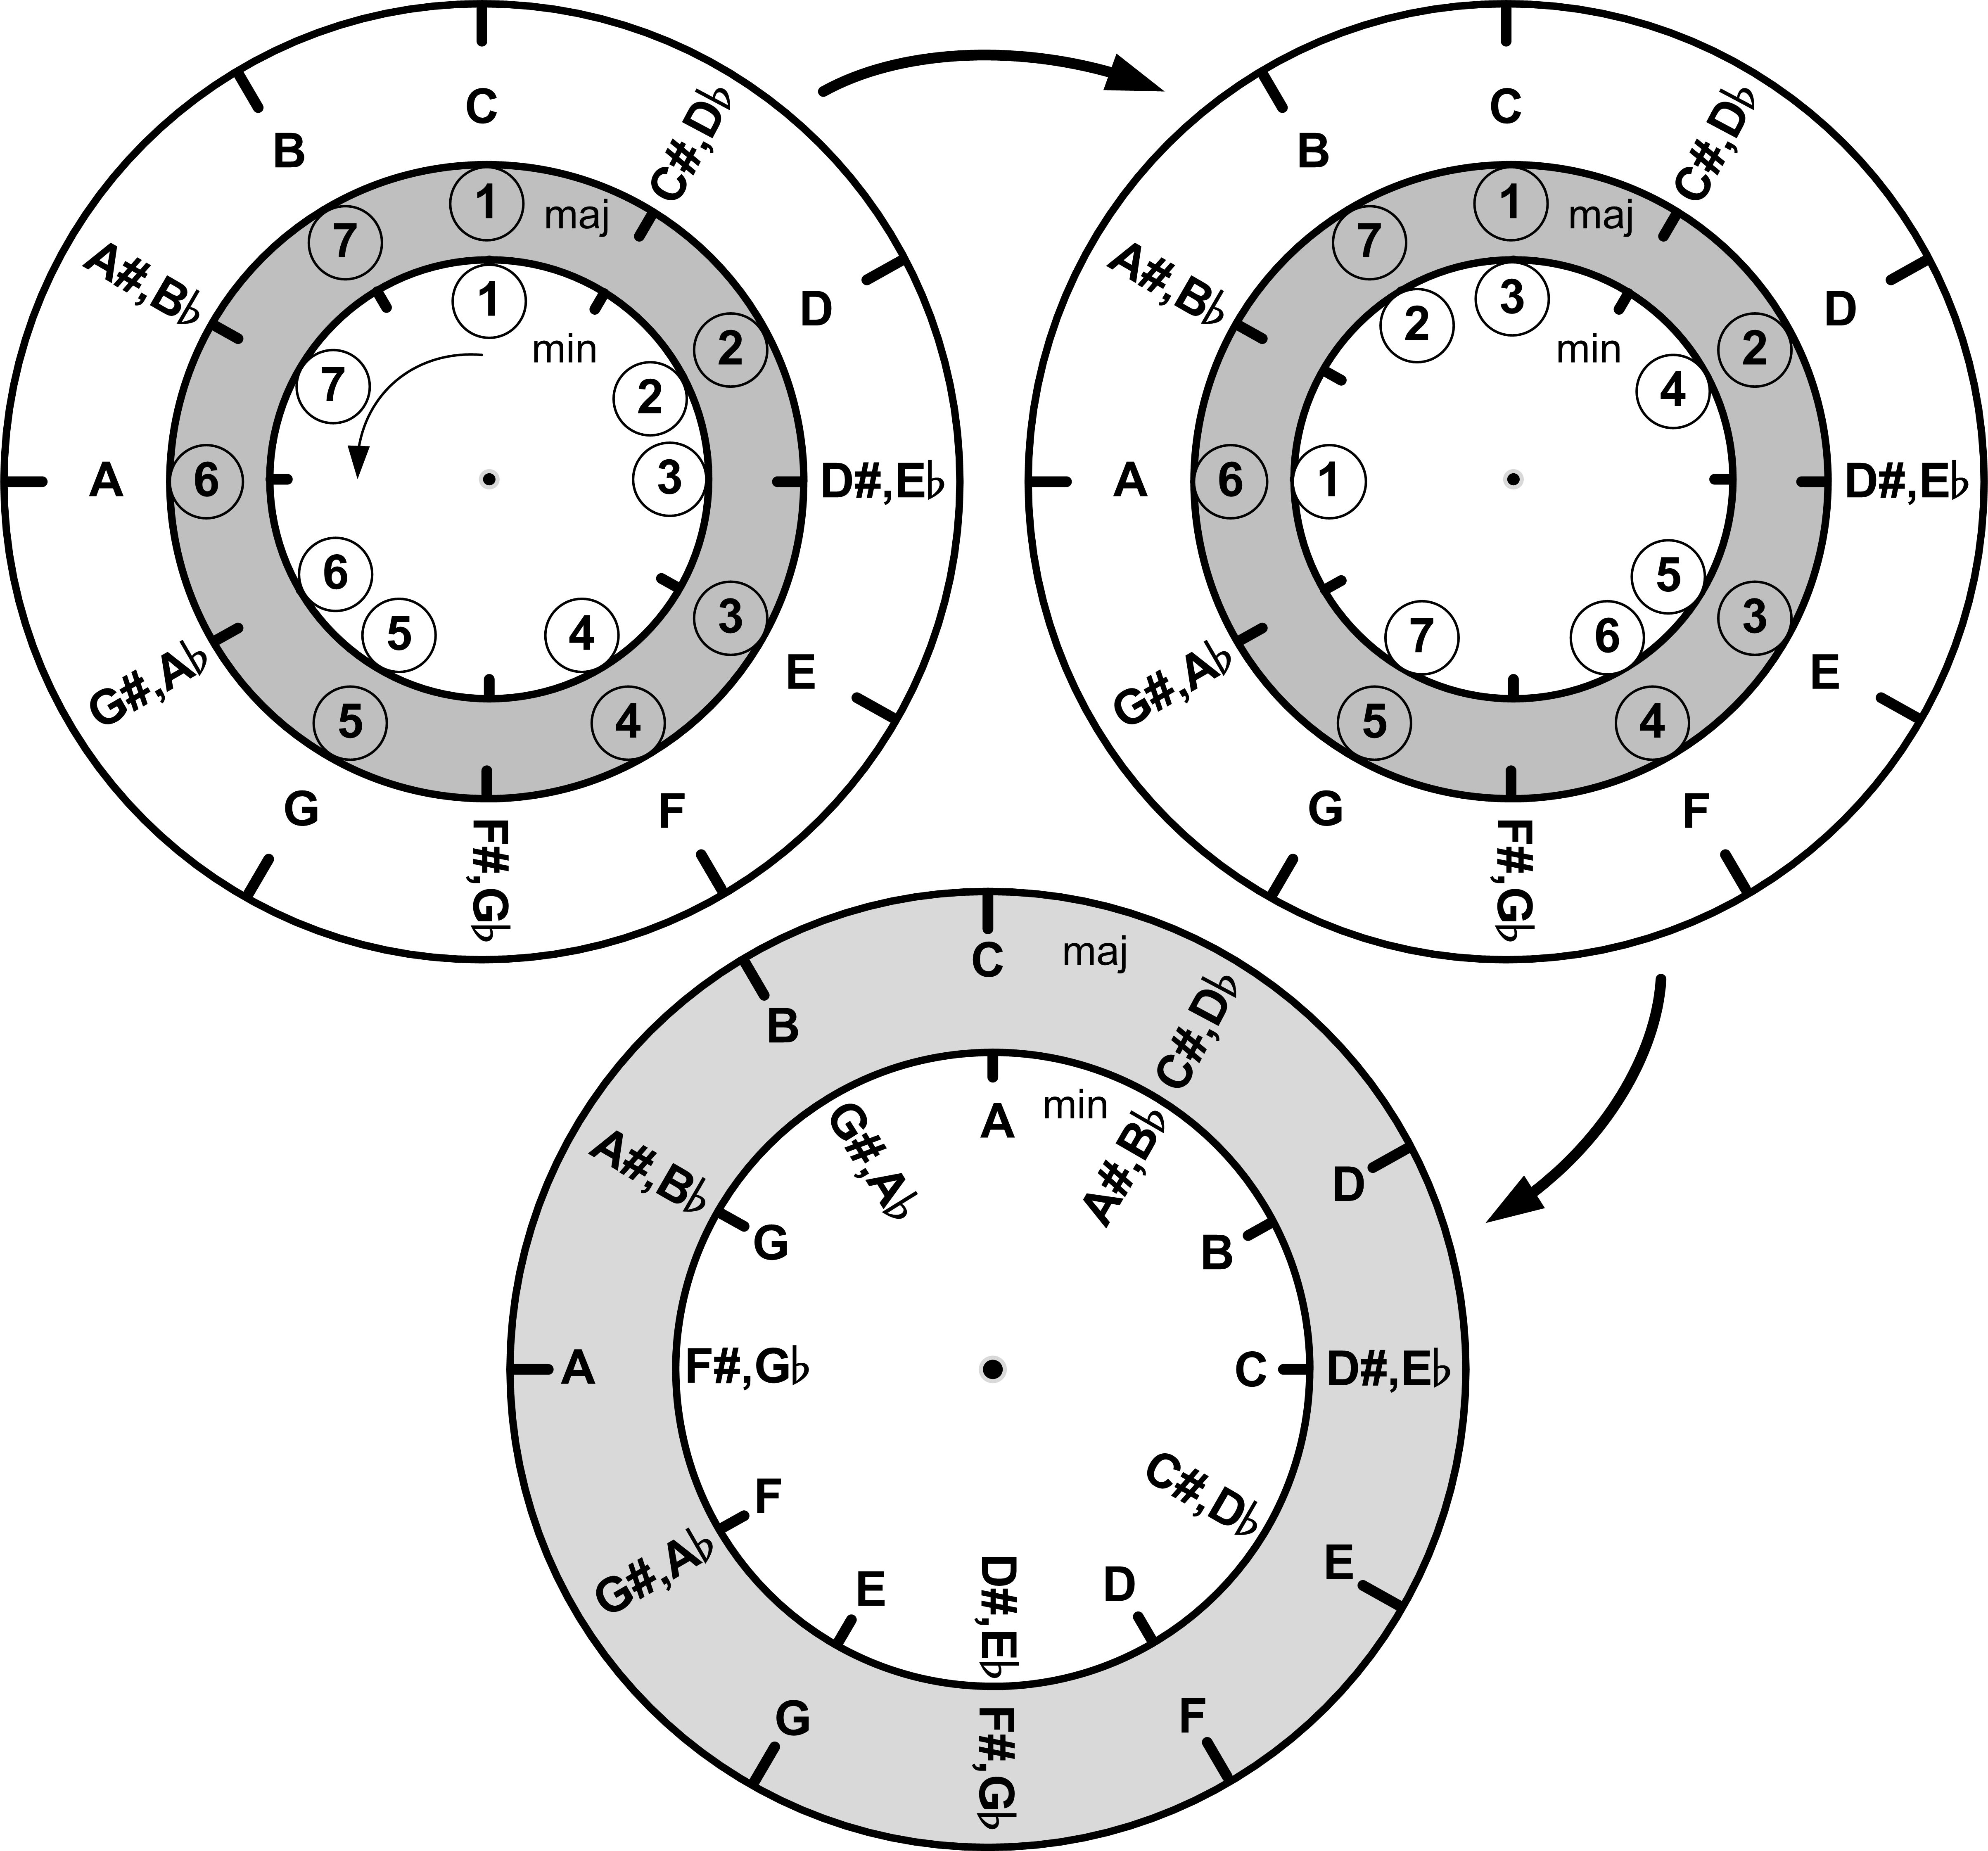
\includegraphics[scale=0.5]{fig/kvinto-kvarto/minor-major-mapping} 
    \caption{Соответствие тоник параллельных мажорных и минорных тональностей}\label{fig:harmony:kvinto-kvarto:minor-major-mapping}
\end{figure}

Если на получившемся приборе совместить шестую ступень мажорного лада с первой ступенью минорного лада (ну или первую ступень мажора с третьей ступенью минора), то будет видно, что они имеют сходную интервальную структуру и порождают параллельные тональности, т.е. тональности, в которые входят одинаковые ноты. Зафиксируем в таком положении кружки со ступенями и будем проворачивать круг с нотами. На рисунке \ref{fig:harmony:kvinto-kvarto:minor-major-mapping} показана ситуация, когда первая ступень мажора указывает на тонику ДО(C), а первая ступень минора --- на тонику ЛЯ(A). ДО-мажор и ЛЯ-минор --- параллельные тональности. Видно, что на внешнем кругу с нотами, тоника параллельной минорной тональности находится на расстоянии трех секторов против часовой стрелки от соответствующей тоники мажорной тональности. Полное соответствие тоник параллельных мажорных и минорных тональностей представлено на рисунке \ref{fig:harmony:kvinto-kvarto:minor-major-mapping}.

Вернемся к нашей <<квинто-квартовой>> перестановке нот и выпишем для неё (во внутренней части круга) тоники параллельных минорных тональностей. Получим предварительный вариант круга, представленный на рисунке \ref{fig:harmony:kvinto-kvarto:kvinto-kvarto-parallel}.

\begin{figure}[!ht]
    \centering
    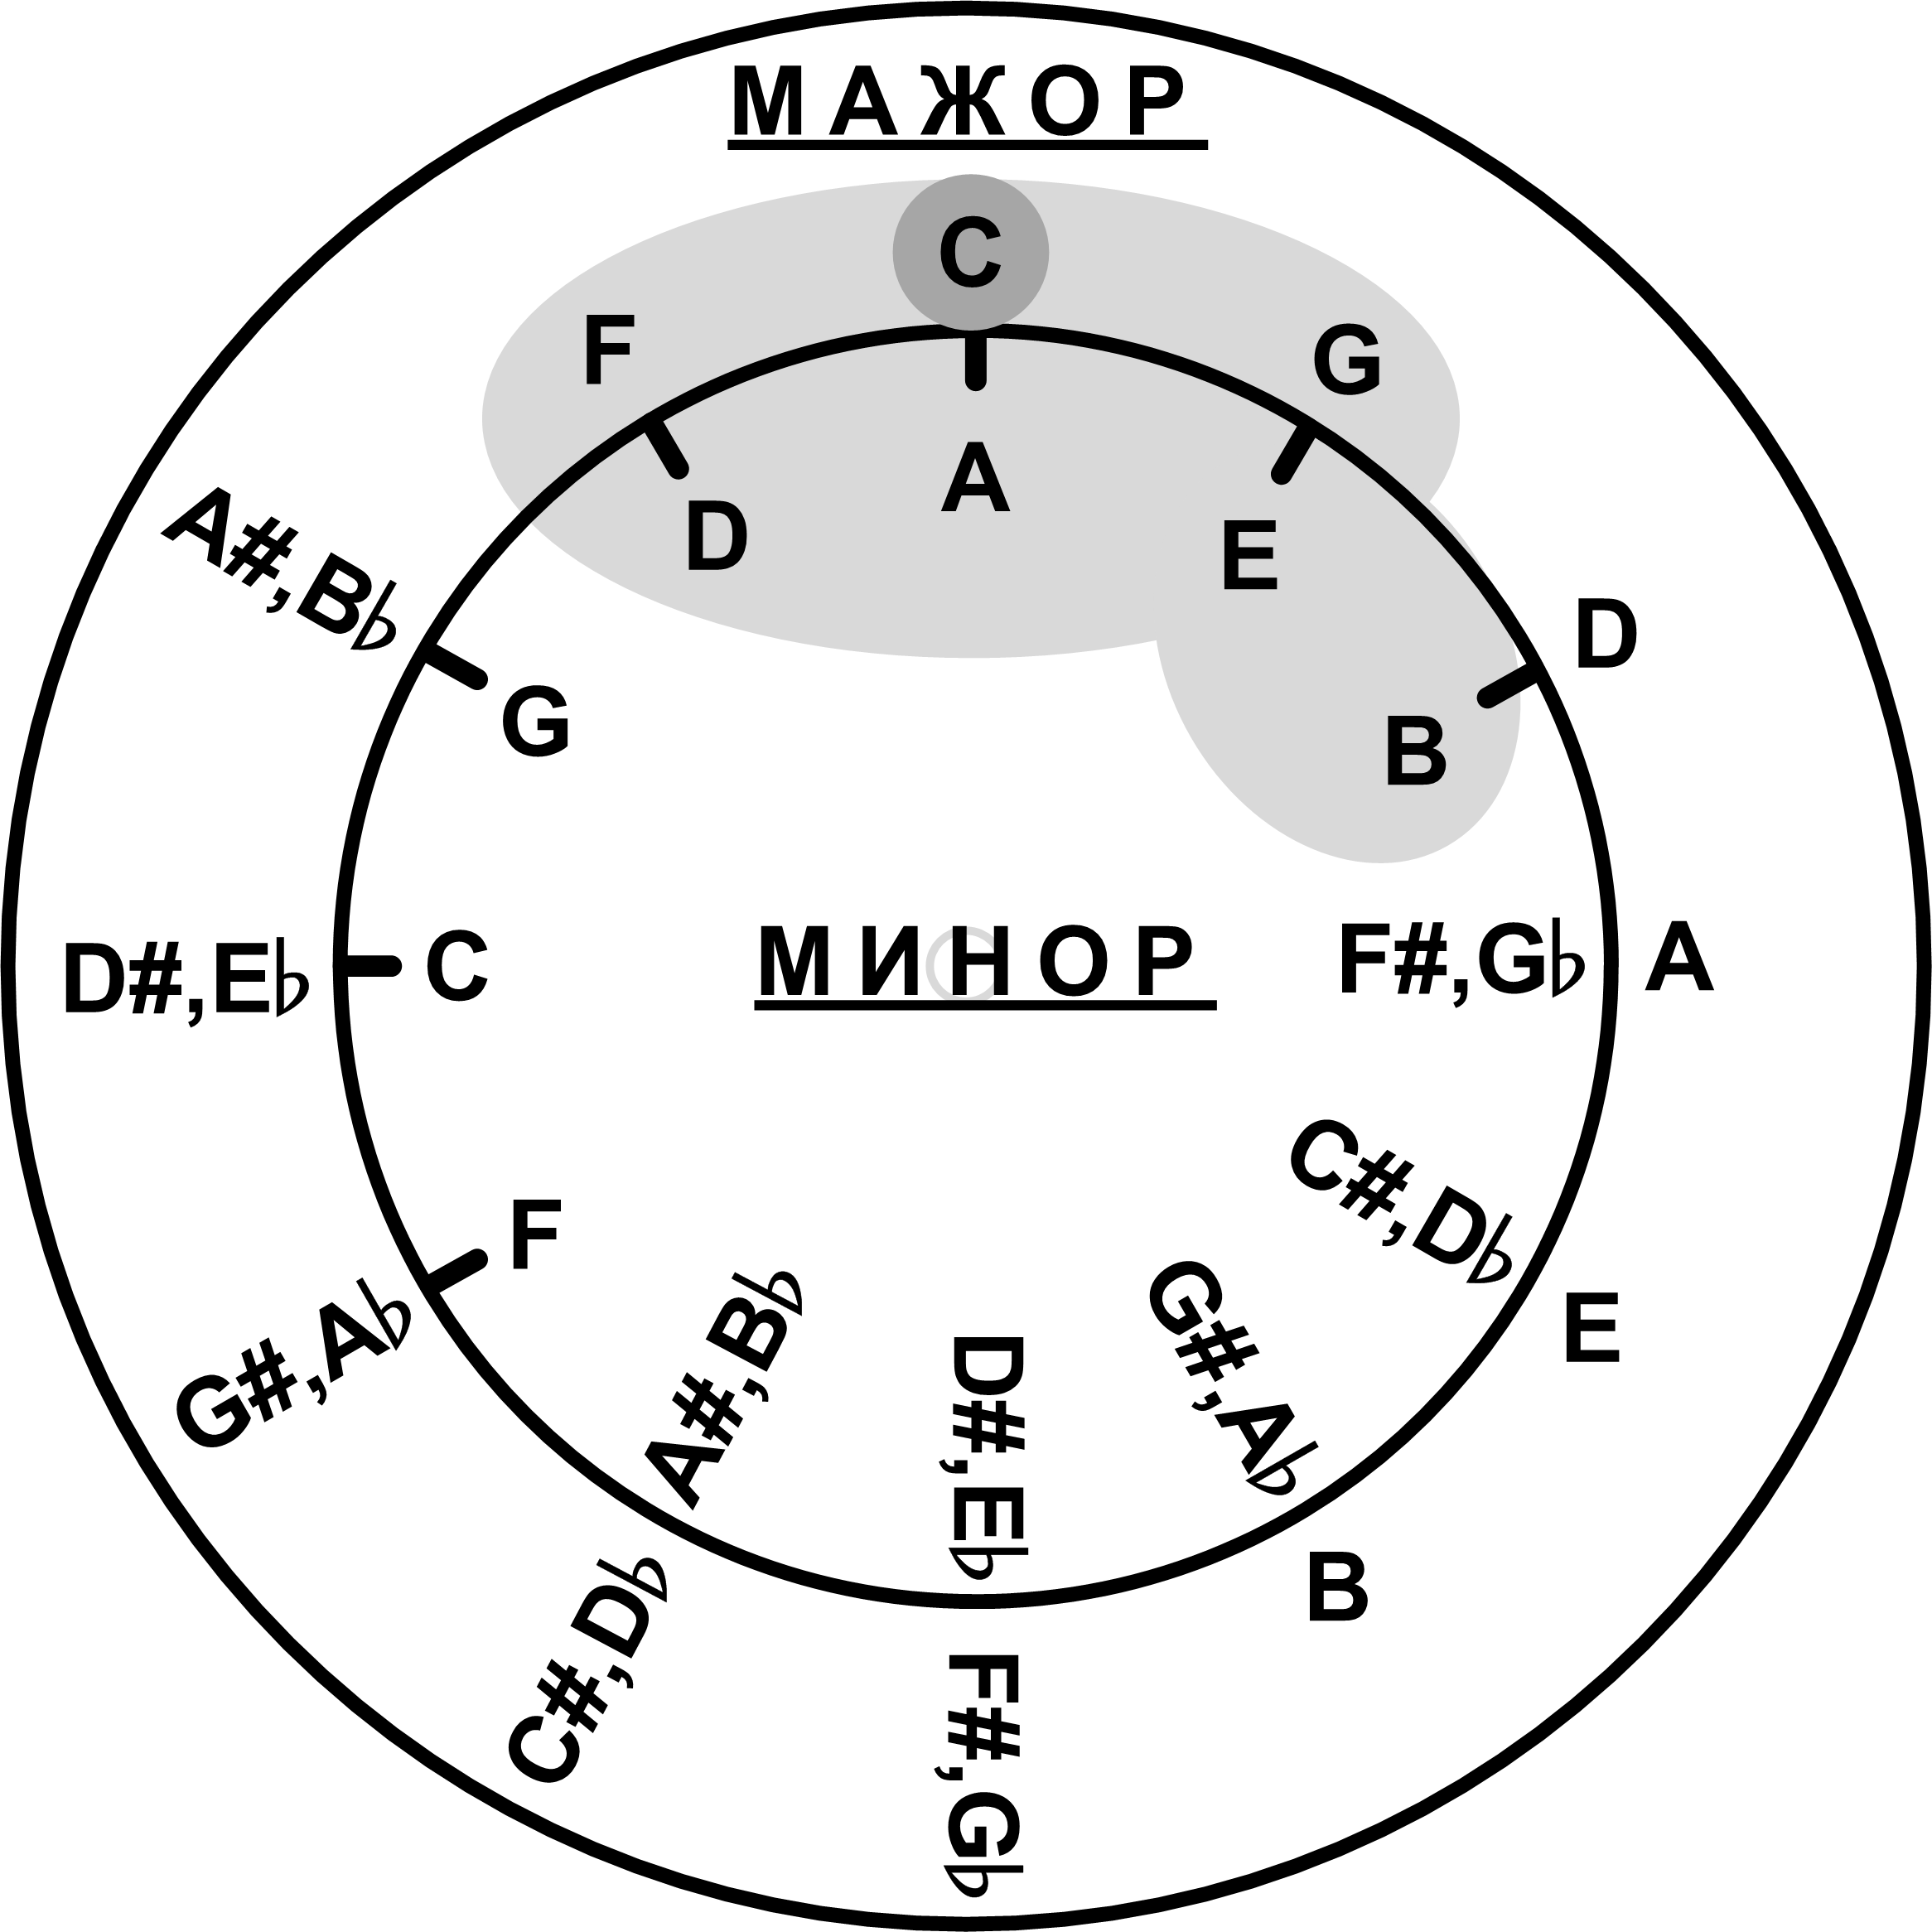
\includegraphics[scale=0.5]{fig/kvinto-kvarto/kvinto-kvarto-parallel} 
    \caption{Квинто-квартовый круг параллельных минорных и мажорных тональностей (базовая версия)}\label{fig:harmony:kvinto-kvarto:kvinto-kvarto-parallel}
\end{figure}

Если приглядеться к рисунку \ref{fig:harmony:kvinto-kvarto:kvinto-kvarto-parallel} внимательнее, то можно увидеть, что внутренний круг нот (параллельные минорные тоники) просто повёрнут на три сектора против часовой стрелки относительно мажорных тоник. Так как и на внутреннем (минорнм), так и на внешнем (мажорном) круге одни и те же ноты идут в одном и том же порядке (они лиш смещены друг относительно друга), то ноты мажорной тональности стало еще проще искать. Например, ноты тональности ДО-мажор выделены на рисунке \ref{fig:harmony:kvinto-kvarto:kvinto-kvarto-parallel} серым цветом. Вам лишь нужно найти мажорную тонику (в примере --- ДО(C), выделена более темным оттенком серого) на внешнем круге и выделить группу соседних нот, а также парных им на <<минорном>> круге, ну и останется добавить еще одну нотку, являющуюся соседкой выделенной группе на минорном круге (по часовой стрелке, в примере ей оказаласт нота СИ(B)).

Ноты минорной тональности найти так же просто: нужно найти тонику на внутреннем, минорном, круге, а затем отметить соответствующую ей тонику мажорной тональности. Всё. Дальше те же действия, что и для поиска нот мажорной тональности\footnote{Когда и если будете упорядочивать ноты минорной тональности по высоте не забудьте взять тонику именно минорной тональности}.

Круг в принципе готов и им уже можно пользоваться, но давайте поможем и академическим кругам! Эти бедняги часто сталкиваются с подобной задачкой. Дано:

\begin{center}    
    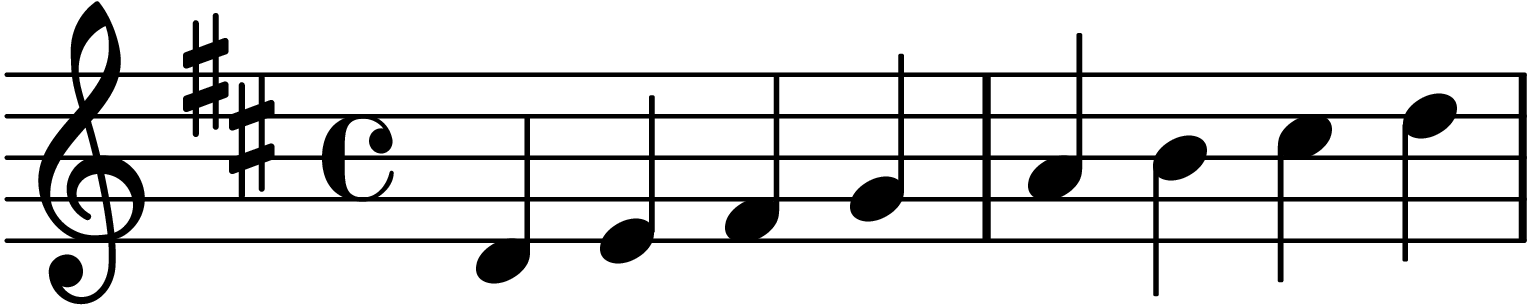
\includegraphics{fig/kvinto-kvarto/tonality-d-maj}
\end{center}

Найти: мажорную тональность, в которой записана <<музыка>>, ориентируясь на знаки альтерации после скрипичного ключа.

Конечно, можно напрячься и определить, что <<под диезом>> находятся ноты ФА(F) и ДО(C). Находим их на мажорном круге. Остальные ноты, стало быть без знаков альтерации, они появятся в последовательности, если двигаться от ФА-диез по мажорному кругу против часовой стрелки и их пять. Мажорная тоника, как мы помним, вторая по счету в последовательности: значит это РЕ(D).

Как говорила Ба в серии рассказов <<Манюня>> Наринэ Абгарян: 
\begin{center}
<<Господибожетымой!!!>> 
\end{center}

Ну или как-то так\ldots Лады, конечно, ладами, но в какой же кошмар они превращают чтение нот!

Чтобы хоть немного упростить себе жизнь, музыканты \emph{договорились} определять тональность по типу и количеству знаков альтерации, встретившихся после ключа. При этом пришлось пойти на некоторые <<технические>> ухищрения. Давайте рассмотрим их на финальной версии круга, изображенной на рисунке \ref{fig:harmony:kvinto-kvarto:kvinto-kvarto-final}.

\begin{figure}[!ht]
    \centering
    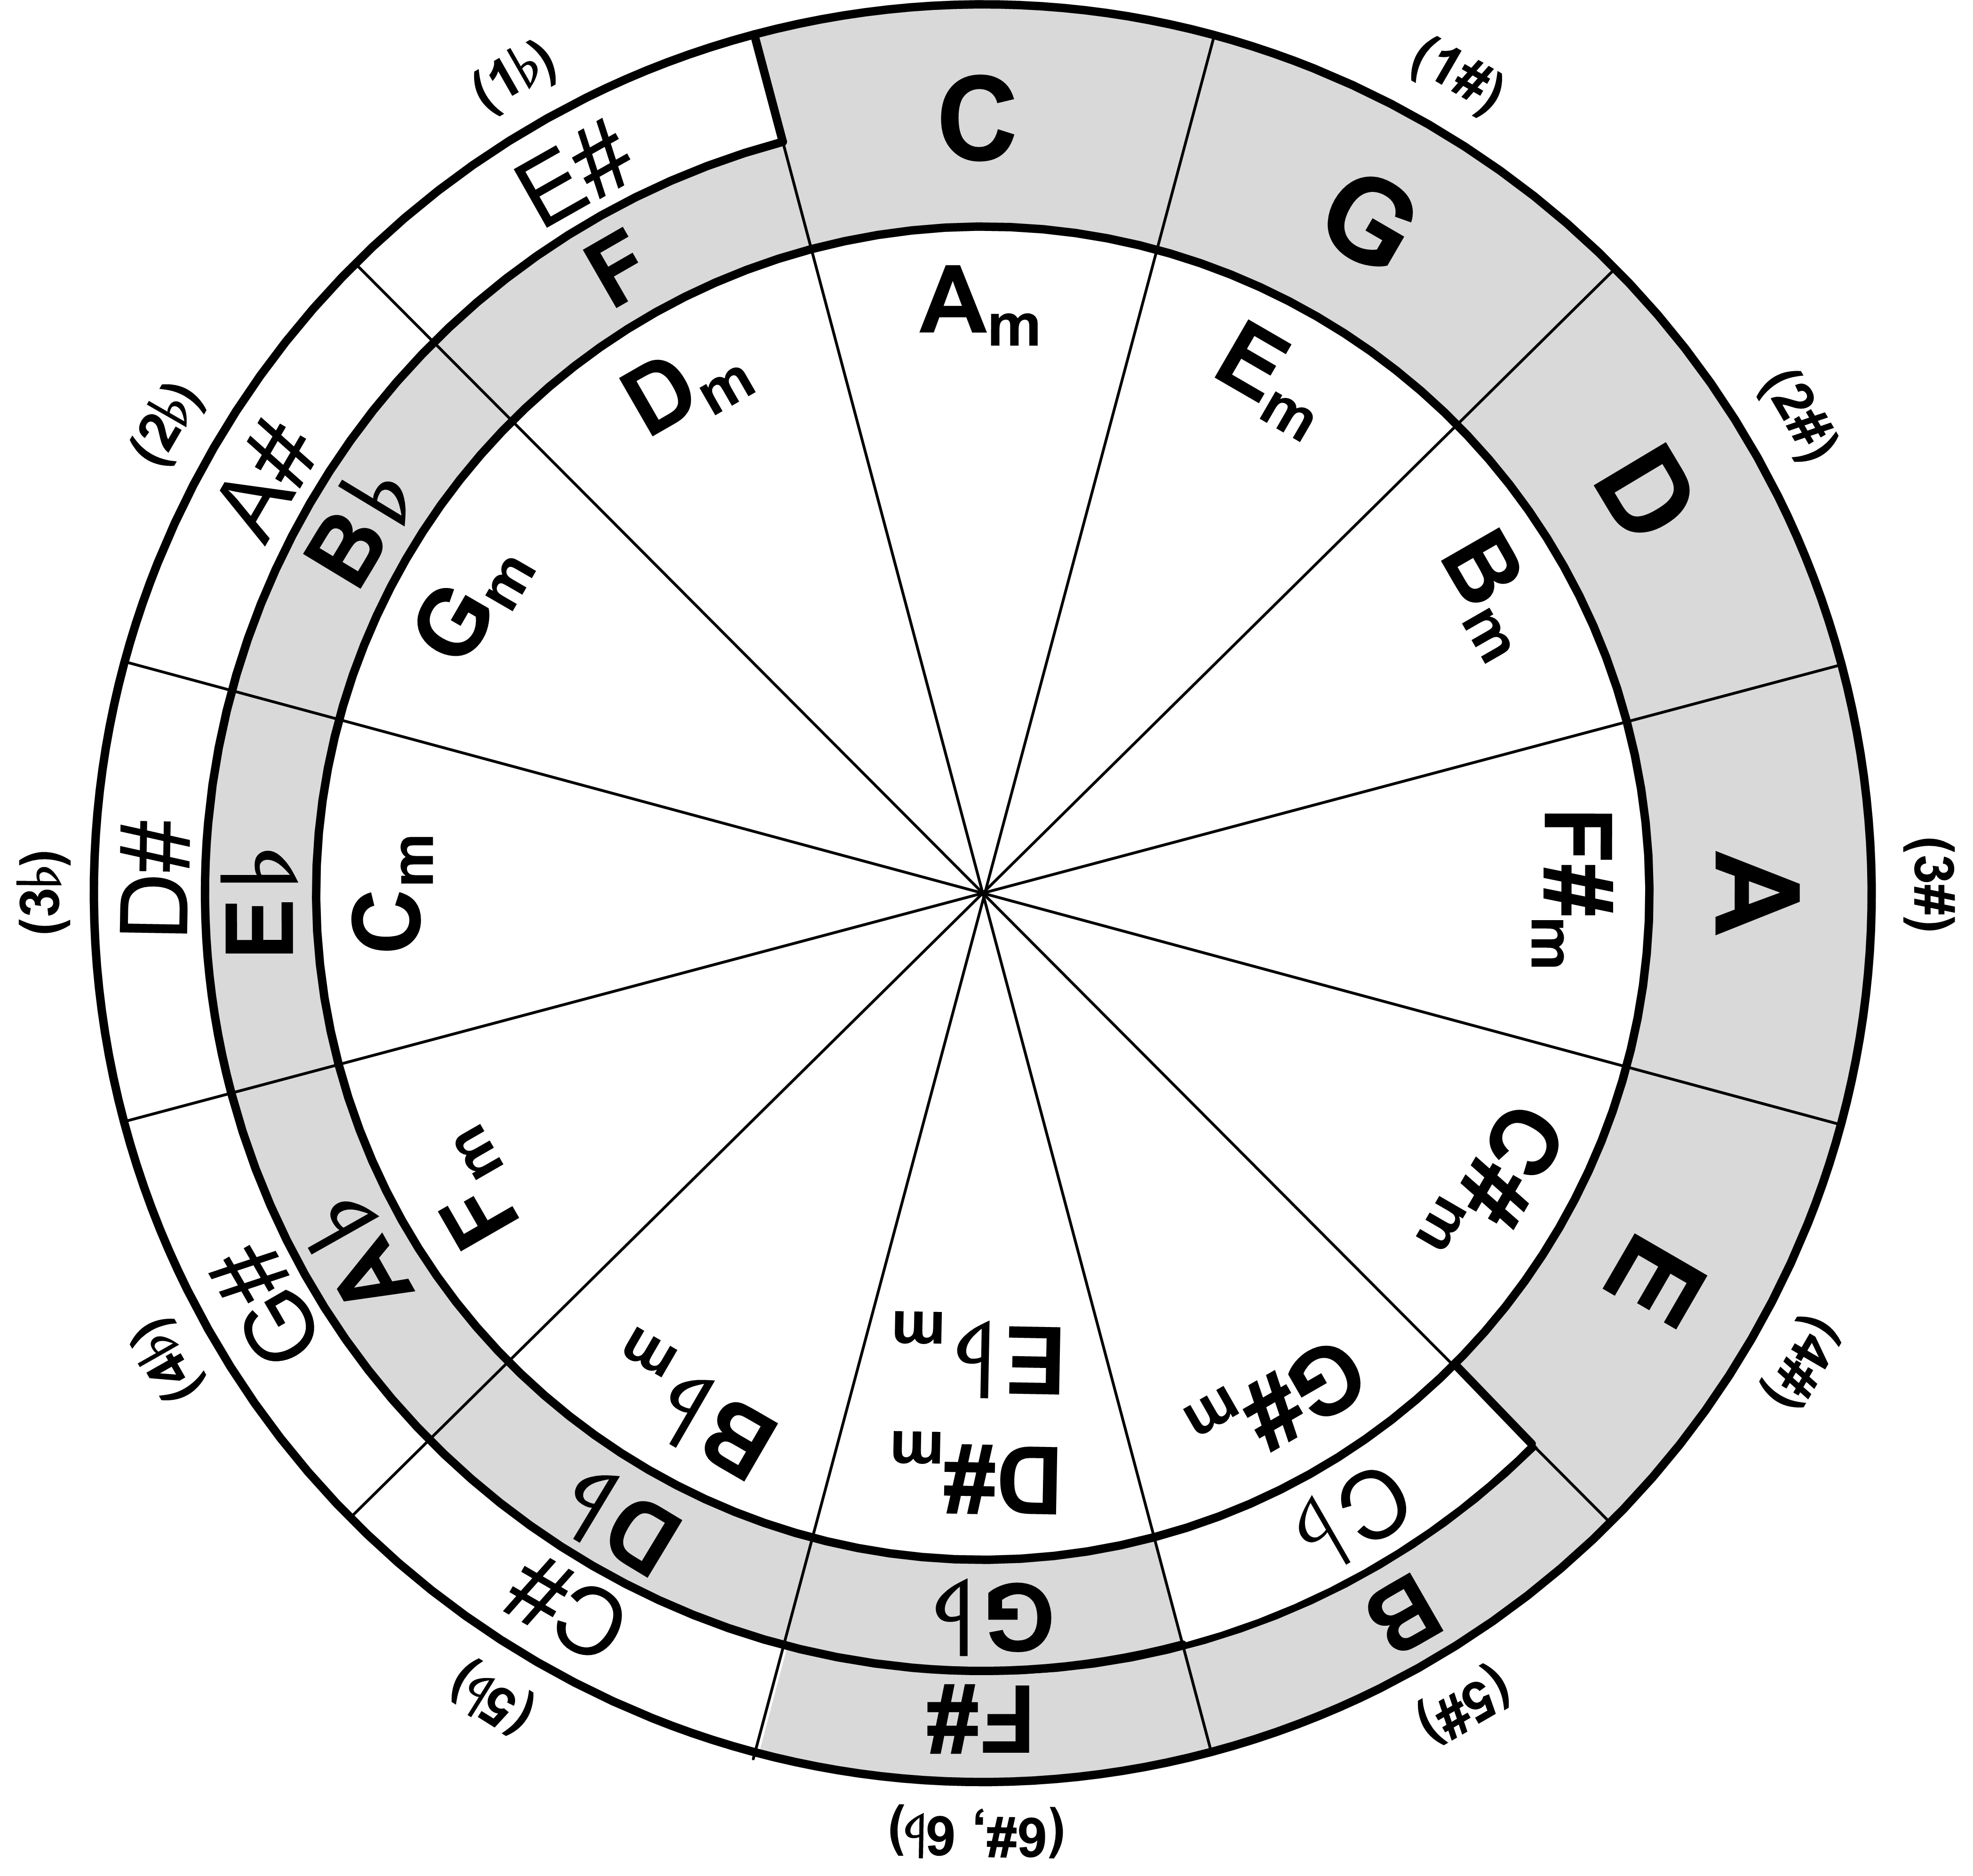
\includegraphics[scale=0.8]{fig/kvinto-kvarto/kvinto-kvarto-final} 
    \caption{Квинто-квартовый круг мажорных и минорных тональностей}\label{fig:harmony:kvinto-kvarto:kvinto-kvarto-final}
\end{figure}

Отметим, что ноты мажорных тональностей образуют теперь своеобразную спираль: 
\begin{itemize}
    \item эта спираль начинает <<наматываться>> по часовой стрелке с ноты ДО-бемоль ($C\flat$);
    
    \item далее как обычно следует привычная группа альтерированных нот, но при этом используется только знак альтерации бемоль ($\flat$):
    \[
        {G\flat}\rightarrow
        {D\flat}\rightarrow
        {A\flat}\rightarrow
        {E\flat}\rightarrow
        {B\flat};
    \]
    
    \item виток продолжается группой нот без знаков альтерации:
    \[
        F\rightarrow
        C\rightarrow
        G\rightarrow
        D\rightarrow
        A\rightarrow
        E\rightarrow
        B;
    \]
    
    \item далее опять начинается привычная группа альтерированных, но теперь только знаком диез ($\sharp$) нот, идущих как бы вторым слоем по аналогичным, альтерированным бемолем ($\flat$) нотам: 
    \[
        {F\sharp}\rightarrow
        {C\sharp}\rightarrow
        {G\sharp}\rightarrow
        {D\sharp}\rightarrow
        {A\sharp}\rightarrow
        {E\sharp}.
    \]
\end{itemize}

Стоит также обратить внимание, что на круге (рисунок \ref{fig:harmony:kvinto-kvarto:kvinto-kvarto-final}) появились <<странные>> ноты $E\sharp$ и $C\flat$. Они нужны, чтобы увеличить количество нот с соотвествующим знаком альтерации до шести, ведь в противном случае по количеству знаков альтерации некоторые тональности различить бы не удалось. Представьте, что например, мы не ввели бы для ноты СИ($B$) её альтерированный аналог ДО-бемоль($C\flat$). Тогда для тональности СОЛЬ-бемоль-мажор $C\flat$-maj мы получили бы набор с пятью альтерированными нотами:
\[
    B\rightarrow
    {G\flat}\rightarrow
    {D\flat}\rightarrow
    {A\flat}\rightarrow
    {E\flat}\rightarrow
    {B\flat}\rightarrow
    F.
\]

Но тогда и тональность РЕ-бемоль-мажор($D\flat$):
\[
    {G\flat}\rightarrow
    {D\flat}\rightarrow
    {A\flat}\rightarrow
    {E\flat}\rightarrow
    {B\flat}\rightarrow
    F\rightarrow
    C
\]
имела бы те же самые пять альтерированных нот, что и ДО-бемоль-мажор: по числу знаков альтерации их бы различить не удалось. А вот с нововведением ДО-бемоль($C\flat$) вместо СИ($B$), тональность СОЛЬ-бемоль-мажор разживется шестью знаками альтерации и спутать её с другой тональностью будет невозможно:
\[
    {C\flat}\rightarrow
    {G\flat}\rightarrow
    {D\flat}\rightarrow
    {A\flat}\rightarrow
    {E\flat}\rightarrow
    {B\flat}\rightarrow
    F.
\]

Ту же сказку можно рассказать и о <<рождении>> МИ-диез ($E\sharp$).

Теперь обратите внимание на пометки количества тех или иных знаков альтерации, идущих по внешней границе круга (в скобках). Если вы увидели нечто подобное:

\begin{center}    
    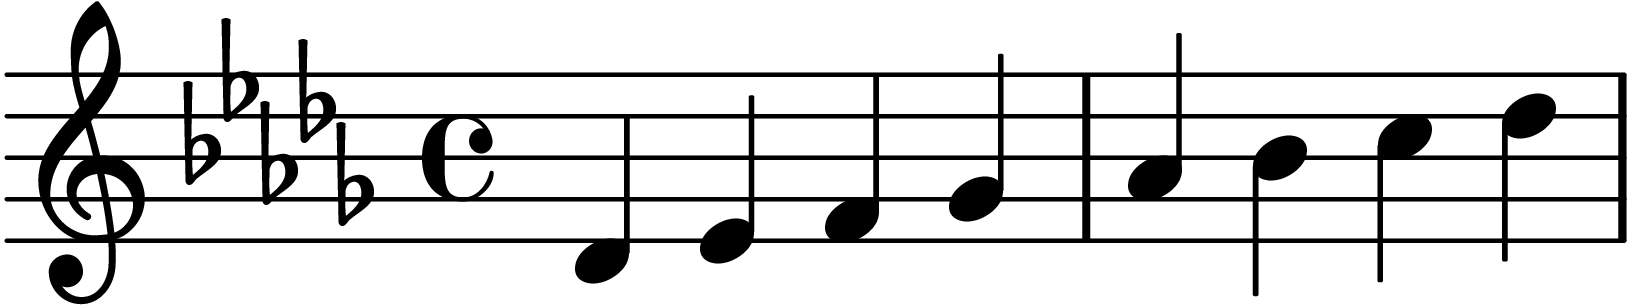
\includegraphics{fig/kvinto-kvarto/tonality-des-maj}
\end{center}

то вам достаточно лишь посчитать количество бемолей и сразу определить, что вы имеете дело с тональностью РЕ-бемоль-мажор($D\flat$-maj), или может быть с параллельной ей СИ-бемоль-минор($B\flat$-min)\ldots

Ну ка:
\begin{center}    
    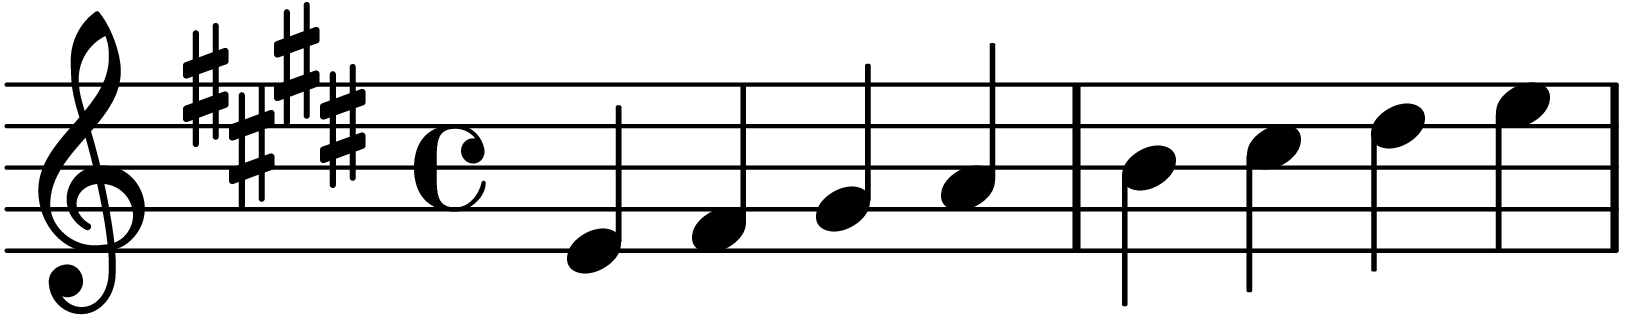
\includegraphics{fig/kvinto-kvarto/tonality-e-maj}
\end{center}
ну да, МИ-мажор($E$-maj) или ДО-диез-минор($C\sharp$-min).

Серым цветом на <<мажорной спирали>> выделены ноты, которые \emph{принято} использовать в качестве тоник мажорных тональностей. Правильно сказать <<ЛЯ-бемоль-мажор>> ($A\flat$-maj), а вот <<СОЛЬ-диез-мажор>> ($G\sharp$-maj) --- уже нарушение этикета, хотя вроде бы полностью однофигственные вещи. Скажете так на музыкальной конференции --- и кто-то из слабых сердцем профессоров может уйти в мир иной от такого невежества. Для обозначения параллельных минорных тоник также используются не все ноты.

Заметили, что для обозначения минорных тоник, использовался индекс <<$m$>>? Стало очень похоже на обозначение минорных аккордов? Действительно, круг очень часто используется именно для подбора аккордов. Например в песне <<Звезда по имени солнце>> используются аккорды: $A_m$, $C$, $D_m$, $G$. Найдите их на круге и поразмышляйте о тональности этой песни.


  %об ладах, интервалах и аккордах
    \chapter{Тройное сальто назад можешь? Трюки и фишечки}
\label{ch:tricks}


\section{А чтоб как капелька упала? Флажолет}
\label{ch:tricks:flageolet}

Флажолетом называется прием игры, позволяющий <<изъять>> из обычного звука оснвоной тон и часть обертонов. В результате получается весьма необычный на слух звук.

Для начала вспомним структуру звука, издаваемого струной, обратившись к рисунку \ref{fig:tricks:flageolet:nodes}. Заметим, что в помеченных на рисунке серыми кружками точках струны колебания отсутствуют --- это узлы колебаний. Первый обертон имеет один узел на струне, второй --- два, и тд.

\begin{figure}[!ht]
    \centering
    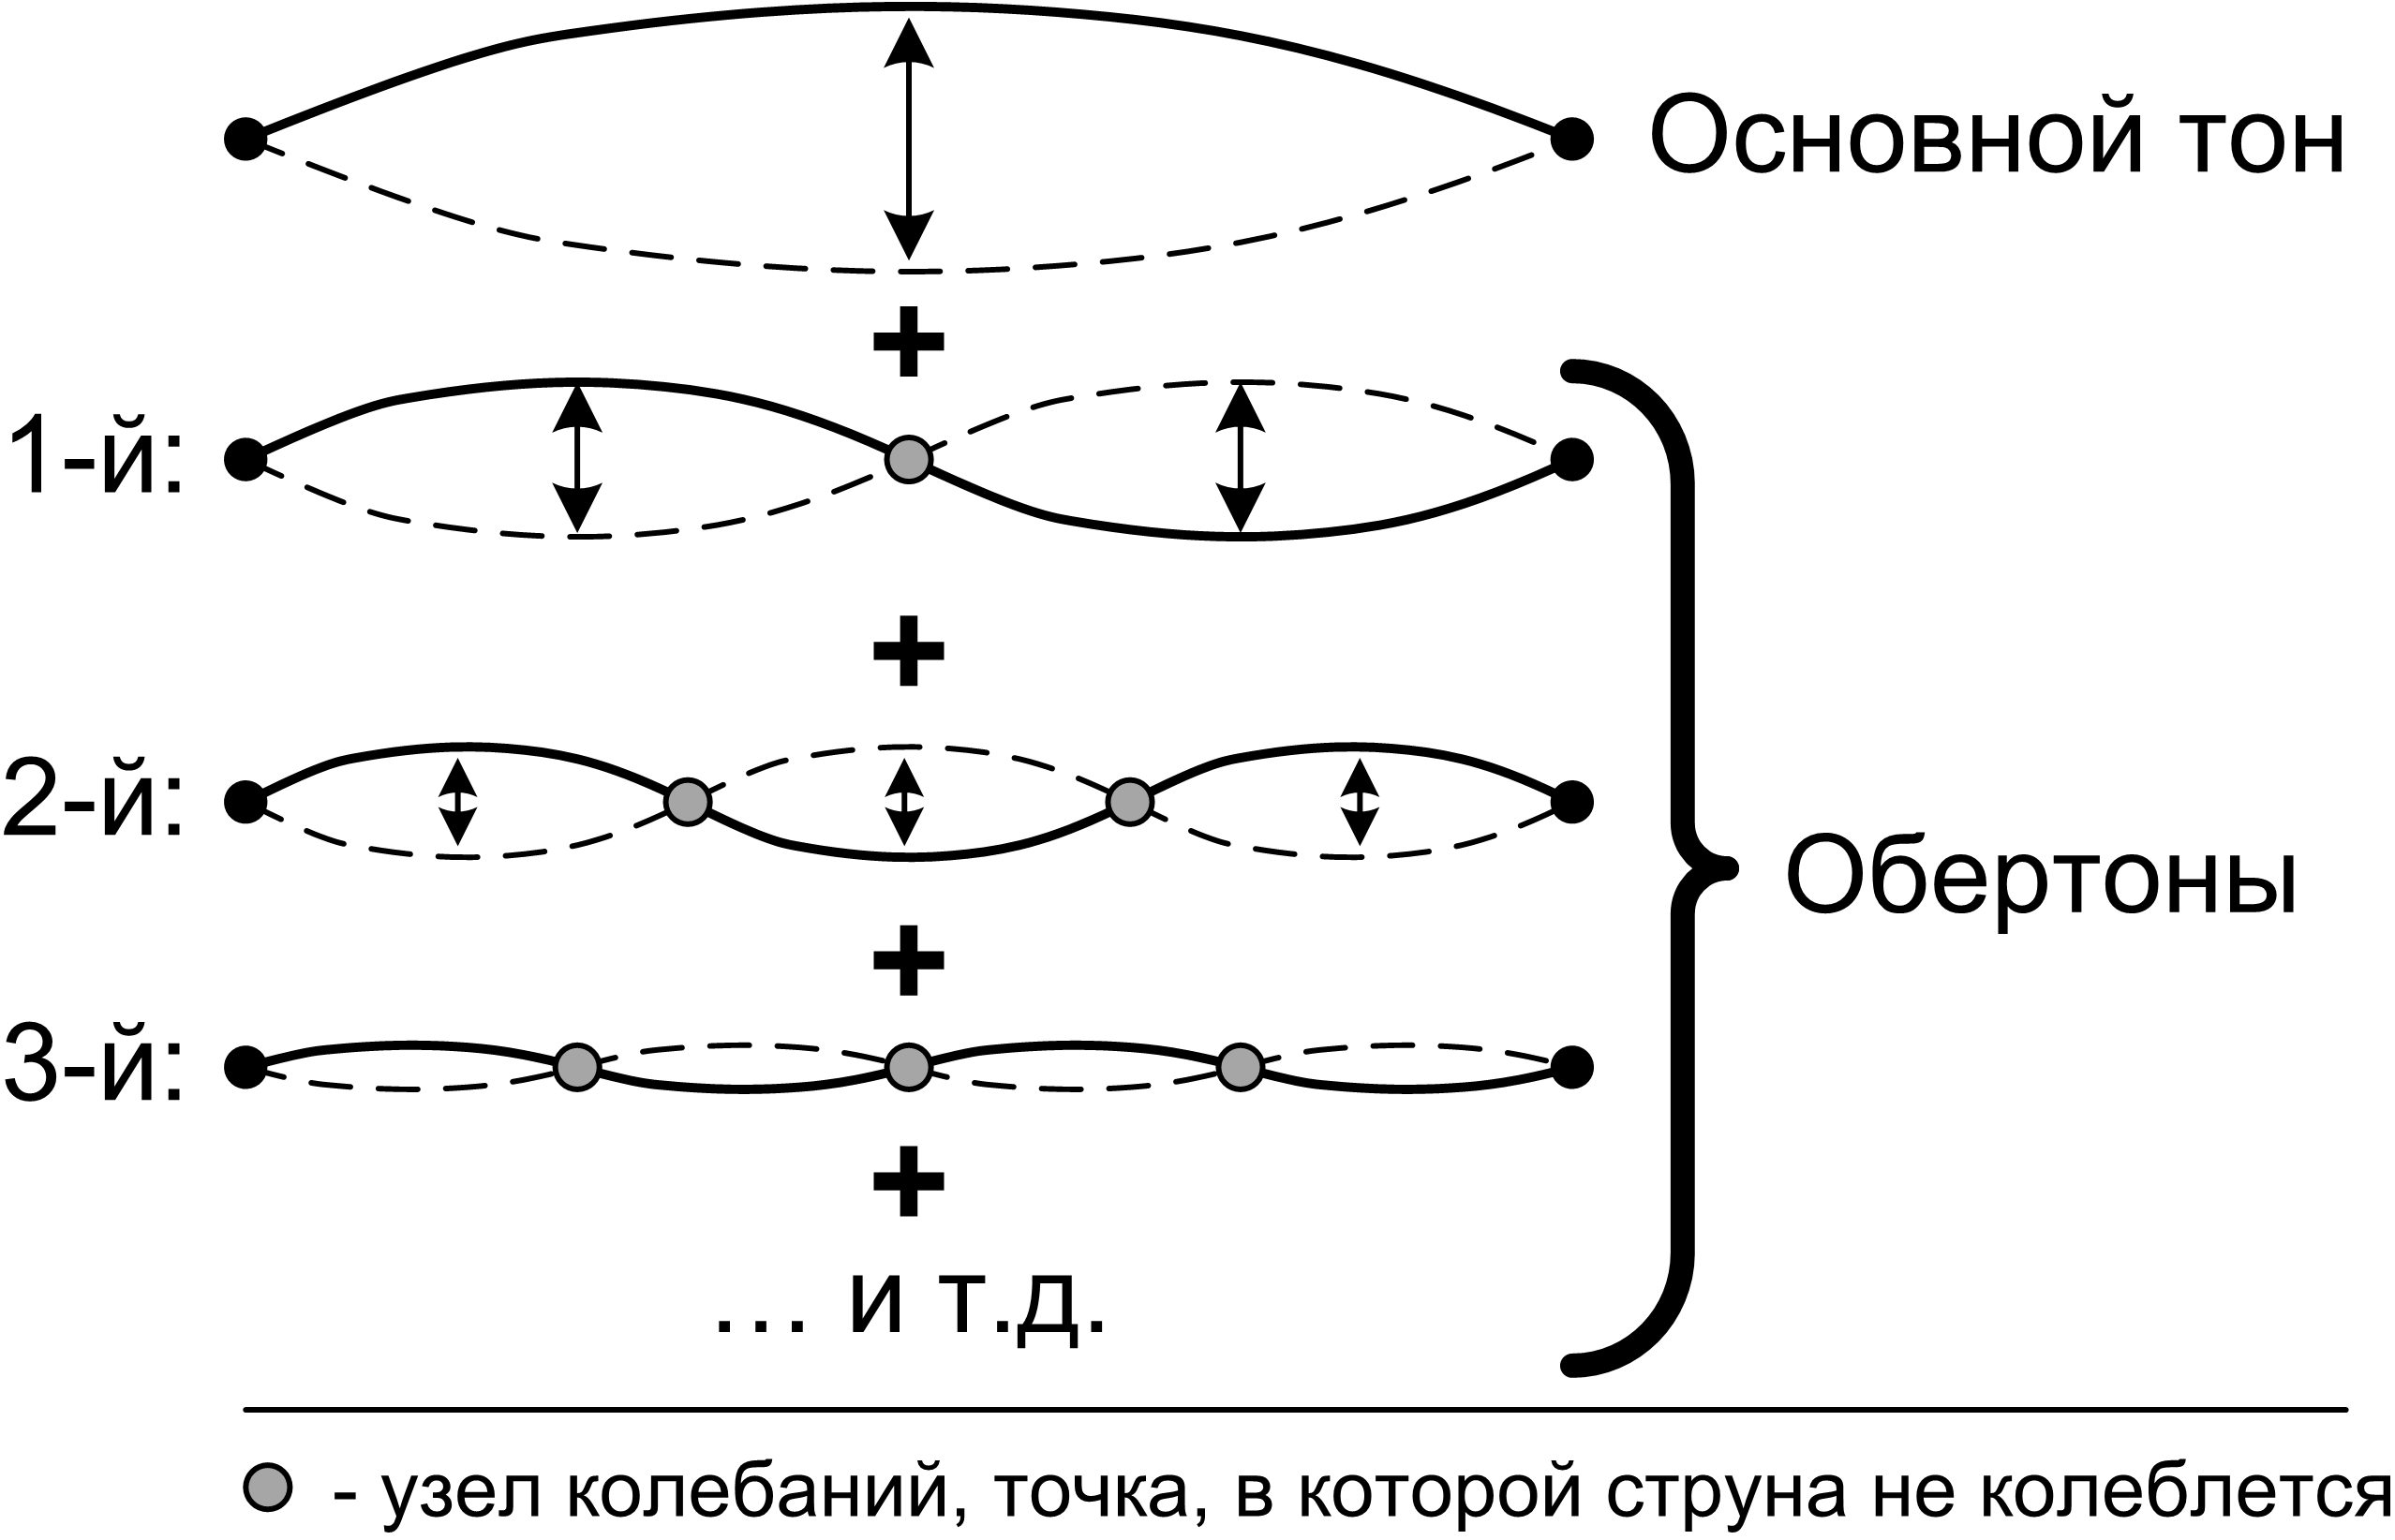
\includegraphics{fig/string-nodes} 
    \caption{Структура звука}\label{fig:tricks:flageolet:nodes}
\end{figure}

\begin{Example}[Сыграем первый флажолет]
    Давайте сыграем флажолет на первой, самой тонкой струне. Там он прозвучит лучше всего. Найдем середину струны --- место, где находится узел первого обертона. Как известно, это прямо над 12-м ладовым порожком. Далее нужно легко поставить палец\footnote{Обычно указательный или средний, какой лучше слушается} левой руки на середину струны, не нужно сильно давить, а тем более прижимать струну к 12-му порожку --- нужно легкое касание. Далее щипните правой рукой струну как обычно, но чуть порезче. Палец левой руки должен уйти с узла вверх на мгновение позже щипка, почти одновременно с ним.
    
    Попробуйте несколько раз, вы поймете, когда у вас получится. Поищите нужное движение, при котором звук получается наиболее ярким.
    
    Причина постоянных неудач: палец левой руки стоит не на узле. 
    
    Если всё получилось, попробуйте сыграть флажолет над 11 или 13-м ладами. Не получается? И не должно. Флажолет - капризная штука, не правда ли?
    
    Что получилось в результате такого приема извлечения звука? Палец левой руки заглушил основной тон, а также все обертоны, не имеющие узла в середине струны. Громче всех (вместо основного тона) прозвучит при этом 1-й обертон.
    
    Разница между сыгранным нами флажолетом и обычным щипком на 12 ладу изображена на рисунке \ref{fig:tricks:flageolet:first}.
\end{Example}
 
\begin{figure}[!ht]
    \centering
    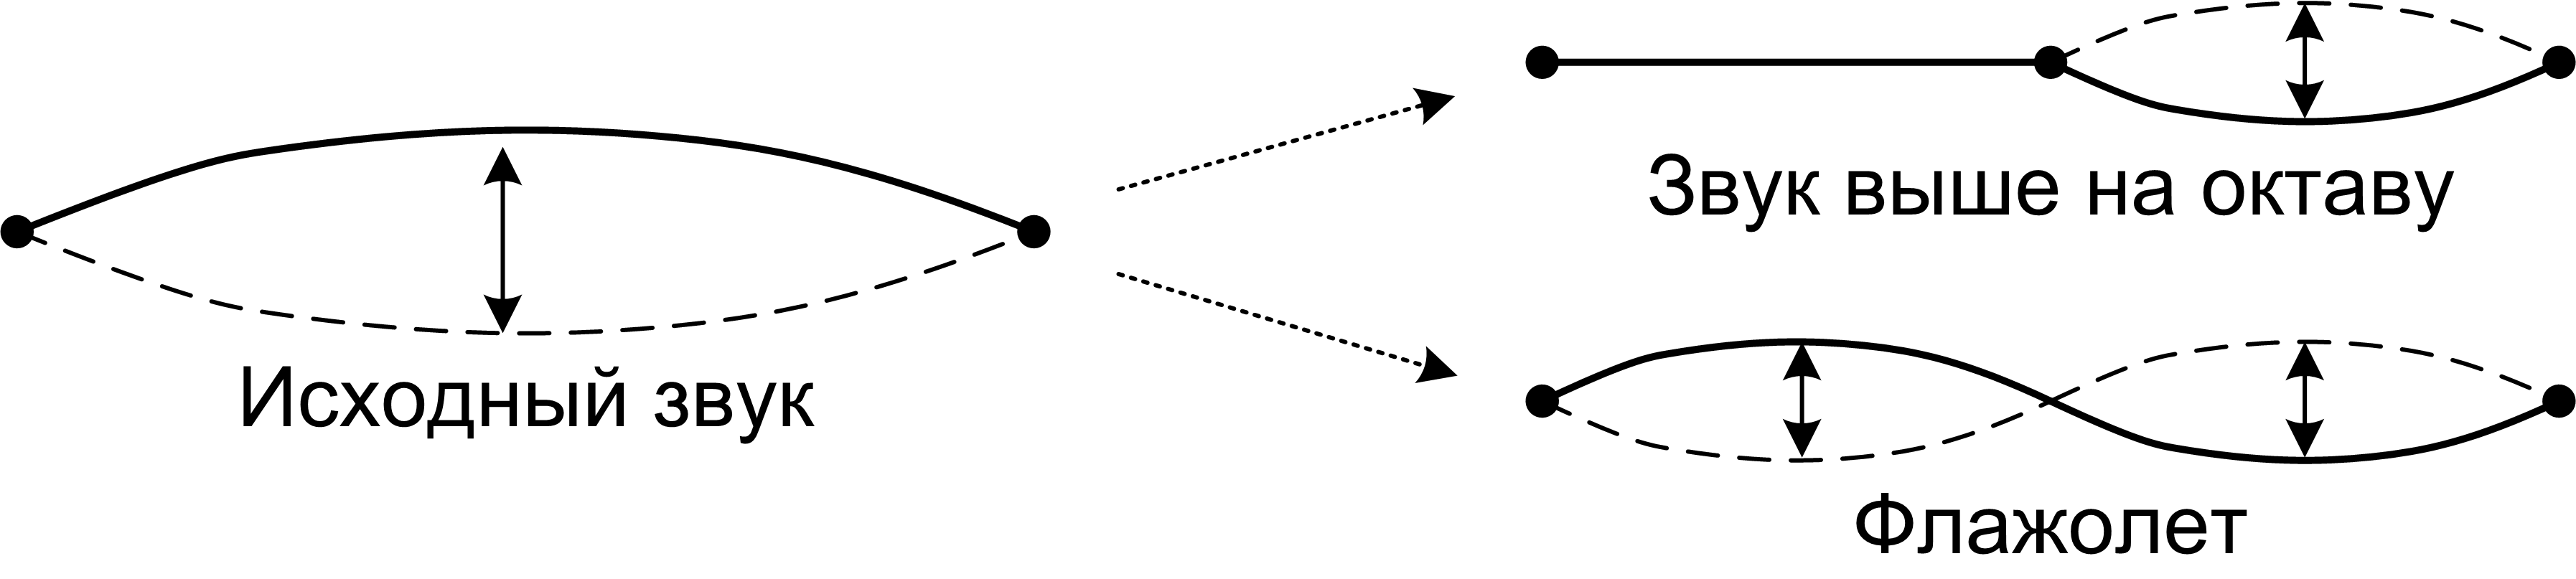
\includegraphics{fig/string-flageolet} 
    \caption{Флажолет первого порядка}\label{fig:tricks:flageolet:first}
\end{figure} 

Этим же приёмом можно сыграть флажолет в узле, делящем струну на три части (см. второй обертон на рисунке \ref{fig:tricks:flageolet:nodes}). В этом случае один из узлов будет находится примерно на 7-м ладу. Давайте проверим, опираясь на формулу \ref{fig:guitar:construction:length} (и помня, что это формула длины струны от подставки до лада):
\[
    L(7)=\frac{L}{(\sqrt[12]{2})^7}\approx L\cdot 0.66742
\]

Тогда как необходимые нам $\frac{2}{3}\cdot L$ составляют:
\[
    \frac{2}{3}\cdot L \approx L\cdot 0.66667
\]

Абсолютная погрешность будет равна $\Delta \approx 0,00075 \cdot L$. Так как длина струны $L$ на полноразмерной классической гитаре составляет $66$ см., то погрешность составит меньше половины миллиметра. Поглядите на свой пухленький пальчик и смело пренебрегайте погрешностью --- ставьте палец левой руки прямо над 7-м ладом.

Играя флажолет на трети струны, вы столкнетесь с еще одним фактором, влияющим на качество звука: флажолет не прозвучит, если правая рука будет щипать струну вблизи второго узла (треть струны от подставки). Поэкспериментируйте. Капризов у флажолета добавилось.

Четверть струны находится примерно над 5-м ладовым порожком\footnote{Буквоеды, посчитайте погрешность}. Не забывайте о наличии уже трех узлов колебаний, вблизи которых нельзя щипать струну правой рукой.

На этом пожалуй можно остановиться, потому что флажолеты более высоких порядков играть все сложнее: они звучат все тише и тише, а вероятность ошибки все больше и больше.

Мы разобрали флажолеты на открытых струнах. Музыканты называют их натуральными или естественными. Так как на практике играют флажолеты в основном на половине струны, и гораздо реже на трети или четверти, то вариантов не слишком-то много.

Представим, что вы зажали струну на первом ладу и она стала короче. На каком ладу теперь находится половина струны? Правильно, на 13-м! Сомневаетесь --- поковыряйте формулу \ref{fig:guitar:construction:length}. На каком бы ладу вы не зажали струну, её половина будет находится на 12 ладов выше, треть --- на 7, четверть --- на 5. Количество мест, где можно сыграть флажолет, резко возросло.

И это, конечно здорово, но если мы зажимаем лад левой рукой, то где взять еще одну руку, чтобы придерживать узел? На открытой струне это делалось левой рукой. Увы, если у вас нет лишней руки, то справляться придется одной правой. Обычно правая рука делает это так: указательным пальцем касается нужного узла, а большим (безымянным или мизинцем, кому как удобнее) играет щипок, практически одновременно с этим снимая с узла указательный палец (проще отнимать ладонь целиком). Знакомьтесь: \emph{искуственный} флажолет.

Все, что сказано, справедливо для аккустических гитар\footnote{В отношении колебаний струны справедливо, конечно и для электрических гитар тоже. Но флажолеты на электрических гитарах играют по-другому. Если задеть колеблющуюся струну на аккустике, то звук исчезнет почти сразу --- слишком много энергии потеряет струна. Но это не значит, что она перестанет колебаться. Таким касанием отфильтруется основной тон и огромное количество обертонов. Останутся только обертоны с узлами в точке касания. Так как электрическая гитара сосет энергию для звука из электрической сети, то её потери энергии струны волнуют гораздо меньше --- больше важен сам факт колебаний. То есть на электрогитаре долго мучаться с поиском нужного узла не надо вовсе --- ткните в любое место на струне и результат будет. Сам флажолет на электрогитаре звучит не так изящно, как на аккустике --- он визжит (словами А. Пушного) <<как сучка>>! Обычно флажолет на электрогитаре играют так: медиатор резко ударяет по струне, его движение продолжается чуть дальше, чем обычно, а один из пальцев правой руки на мгновение касается струны}.
   %нестандартные способы звукоизвлечения 
    \chapter*{В заключение}
\addcontentsline{toc}{chapter}{В заключение}

Данный текст подготовлен в издательской системе {\LaTeXe} (автор использовали MiC\TeX.). Эта издательская система является стандартом де факто в научных и технических кругах.

Заинтересовавшимся версткой в {\LaTeX} можно рекомендовать следующие книги: \cite{bib:cotelnikov,bib:baldin}.

Про предшественника {\LaTeX} --- программу {\TeX} следует читать бестселлер от автора\footnote{{\TeX} на самом деле является ядром \LaTeX} \cite{bib:knuth:AllAbout}.
    %заключение
    
    \bibliographystyle{plain}
    \bibliography{./bibliobase}
\end{document} %конец документа
